%%%%%%%%%%%%%%%%%%%%%%%%%%%%%%%%%%%%%%%%%
% PESTI Report Class File 
%
% Adapted to PESTI/ISEP style (April/2024) by 
%  Elsa Ferreira Gomes (efg@isep.ipp.pt) and 
%  Jorge Coelho (jmn@isep.ipp.pt)
% Updates:
%  - March/2025: António Barros (amb@isep.ipp.pt)
%%%%%%%%%%%%%%%%%%%%%%%%%%%%%%%%%%%%%%%%%%%%
% TMDEI Dissertation
% LaTeX Template
% Version 0.1 (Dec/2015)
%
% Adapted to TMDEI/ISEP style (Dec/2015) by
%  Nuno Pereira (nap@isep.ipp.pt) and
%  Paulo Baltarejo (pbs@isep.ipp.pt)
%
% Based on MastersDoctoralThesis Version 1.2 by Vel (vel@latextemplates.com) and
% Johannes Böttcher, downloaded from (21/11/15):
% http://www.LaTeXTemplates.com
%
% This template is originally based on a template by:
% Steve Gunn (http://users.ecs.soton.ac.uk/srg/softwaretools/document/templates/)
% Sunil Patel (http://www.sunilpatel.co.uk/thesis-template/)
%
% Template license:
% CC BY-NC-SA 3.0 (http://creativecommons.org/licenses/by-nc-sa/3.0/)
%
%%%%%%%%%%%%%%%%%%%%%%%%%%%%%%%%%%%%%%%%%
%https://www.overleaf.com/project/5bfd7e508cfbf932785021c9
%----------------------------------------------------------------------------------------
%	PACKAGES AND OTHER DOCUMENT CONFIGURATIONS
%----------------------------------------------------------------------------------------

\documentclass[
	11pt, % The default document font size, options: 10pt, 11pt, 12pt
	%oneside, % Two side (alternating margins) for binding by default, uncomment to switch to one side (for drafting/reading purposes)
	%english, % english for English;
	portuguese,% for Portuguese; delete temporary files if you change language (e.g. 'make clean; make')
	singlespacing, % Single line spacing, alternatives: onehalfspacing or doublespacing (for drafting/reading purposes)
	%draft, % Uncomment to enable draft mode (no pictures, no links, overfull hboxes indicated)
	%nolistspacing, % If the document is onehalfspacing or doublespacing, uncomment this to set spacing in lists to single
	liststotoc, % Uncomment to add the list of figures/tables/etc to the table of contents (recommended)
	%toctotoc, % Uncomment to add the main table of contents to the table of contents (not recommended)
	parskip, % Add space between paragraphs (recommended)
	%nohyperref, % Uncomment to not load the hyperref package (not recommended)
	nohyperreflinkcolor, % hyperref links are not colored (comment to color links, for example to produce an electronic-only version)
	%headsepline, % Uncomment to get a line under the header
]{PESTI-style} % The class file specifying the document structure

%\usepackage{tikz} % no longer used - AWS physical view replaced with PNG
%\usetikzlibrary{arrows} % Required for fancy arrows in TiKZ graphics (can be removed if not used)
\setcounter{secnumdepth}{3} % Number subsubsections, e.g. 3.4.3.1, as required for architectural decomposition.

\usepackage{pgfplots} % Required for drawing high--quality function plots (can be removed if not used)
\pgfplotsset{compat=newest}
\setlength{\emergencystretch}{2em} % Give LaTeX a little flexibility to avoid small margin overflows.

%
% Next you have examples of admissable citation styles; we recomend using the authoryear-comp citation style (which resembles Harvard); don't forget to only uncomment one
%

% authoryear-comp: recommended citation style (e.g. (Buendía, 1860), (Buendía 1910, Arcadio 1940))
%\usepackage[style=authoryear-comp,backend=biber]{biblatex} % Bibtex backend with the authoryear-comp citation style (authoryear citations, bibliography ordered alphabetically)

% numeric citation style (e.g. [1], [1-3])
\usepackage[style=ieee]{biblatex} % IEEE citation style (numeric citations [1], bibliography ordered by appearance)
\setcounter{biburlnumpenalty}{9000}
\setcounter{biburllcpenalty}{9000}
\setcounter{biburlucpenalty}{9000}

% alphabetic citation style (e.g. [Buendía10], [Buendía10, Arcadio40])
%\usepackage[style=alphabetic,sorting=none,backend=biber]{biblatex} % Bibtex backend with the alphabetic citation style (alphabetic citations, bibliography ordered by appearance)


\addbibresource{mainbibliography.bib} % The filename of the bibliography

\makeglossaries % build the glossary


%----------------------------------------------------------------------------------------
%	THESIS INFORMATION
%----------------------------------------------------------------------------------------

\thesistitle{Desenvolvimento de um Backoffice Multiaplicação para o Ecossistema OnlyHighIQ: Aplicação à JustCauses} % Your thesis title, this is used in the title, print it elsewhere with \ttitle

\thesisinstitution{OnlyHighIQ} % Where the internship took place, this is used in the title, print it elsewhere with \tinstitution

\thesisacademicyear{2025/2026} % Academic year, e.g. "2024/2025"

\studentname{Tiago Pedroso Silva} % Your name, this is used in the title page, print it elsewhere with \authorname

\studentnumber{1230900} % Student number, e.g. "1209999"

\supervisor{Paulo Maio} % Academic supervisor at ISEP

\externalsupervisor{Rui Cruz} % External supervisor at the internship institution, if exists; comment this line if does not exist.

\examdate{Junho de 2026} % Exam month/year date, e.g. "Abril de 2025"

\keywords{Backoffice, Multiaplicação, Autorização, Auditoria, React, AWS} % Please define up to 6 keywords that better describe your work, print it elsewhere with \keywordnames


\hypersetup{pdftitle=\ttitle} % Set the PDF's title to your title
\hypersetup{pdfauthor=\author} % Set the PDF's author to your name
\hypersetup{pdfkeywords=\keywordnames} % Set the PDF's keywords to your keywords



%----------------------------------------------------------------------------------------
%	THE DOCUMENT STARTS HERE
%----------------------------------------------------------------------------------------

\begin{document}

%----------------------------------------------------------------------------------------
%	FRONT MATTER
%----------------------------------------------------------------------------------------

% Include the frontmatter of your thesis here
% we include the glossary here (frontmatter is included with \input, so this command is as if it was in main.tex)
%All acronyms must be written in this file.

% Institutional
\newacronym{ISEP}{ISEP}{Instituto Superior de Engenharia do Porto}
\newacronym{UC}{UC}{Unidade Curricular}
\newacronym{PESTI}{PESTI}{Projeto/Estágio}
\newacronym{LEI-PROJ}{LEI-PROJ}{Projeto em Licenciatura em Engenharia Informática}

% Cloud & Infrastructure
\newacronym{AWS}{AWS}{Amazon Web Services}
\newacronym{CI/CD}{CI/CD}{Continuous Integration / Continuous Deployment}
\newacronym{SES}{SES}{Simple Email Service}
\newacronym{WAF}{WAF}{Web Application Firewall}
\newacronym{JWKS}{JWKS}{JSON Web Key Set}

% Development & Architecture
\newacronym{API}{API}{Application Programming Interface}
\newacronym{REST}{REST}{Representational State Transfer}
\newacronym{CRUD}{CRUD}{Create, Read, Update, Delete}
\newacronym{E2E}{E2E}{End to End}
\newacronym{FURPS+}{FURPS+}{Functionality, Usability, Reliability, Performance, Supportability}
\newacronym{MVP}{MVP}{Minimum Viable Product}
\newacronym{UI}{UI}{User Interface}
\newacronym{UX}{UX}{User Experience}
\newacronym{QA}{QA}{Quality Assurance}
\newacronym{IA}{IA}{Inteligência Artificial}

% Database
\newacronym{PostgreSQL}{PostgreSQL}{PostgreSQL Relational Database}

% Security & Identity
\newacronym{KYC}{KYC}{Know Your Customer}
\newacronym{KYB}{KYB}{Know Your Business}
\newacronym{MFA}{MFA}{Multi-Factor Authentication}
\newacronym{RBAC}{RBAC}{Role-Based Access Control}
\newacronym{TTL}{TTL}{Time To Live}

% Metrics
\newacronym{KPI}{KPI}{Key Performance Indicator}

% Protocols & Diagrams
\newacronym{HTTP}{HTTP}{Hypertext Transfer Protocol}
\newacronym{SD}{SD}{Sequence Diagram}
\newacronym{SSD}{SSD}{System Sequence Diagram}
\newacronym{SSE}{SSE}{Server-Sent Events}

% Other
\newacronym{CSV}{CSV}{Comma-Separated Values}
\newacronym{OJC}{OJC}{Only Just Causes}
\newacronym{PDF}{PDF}{Portable Document Format}


\frontmatter % Use roman page numbering style (i, ii, iii, iv...) for the pre-content pages

\pagestyle{plain} % Default to the plain heading style until the thesis style is called for the body content

%----------------------------------------------------------------------------------------
%	TITLE PAGE
%----------------------------------------------------------------------------------------

\maketitlepage


%----------------------------------------------------------------------------------------
%	STATEMENT of INTEGRITY
%----------------------------------------------------------------------------------------
\integritystatement

%----------------------------------------------------------------------------------------
%	DEDICATION  (optional)
%----------------------------------------------------------------------------------------
%
%\dedicatory{For/Dedicated to/To my\ldots}
%\begin{dedicatory}
%\end{dedicatory}

%----------------------------------------------------------------------------------------
%	ABSTRACT PAGE
%----------------------------------------------------------------------------------------

\begin{abstract}

Qualquer aplicação que pretende ser utilizada em larga escala, por diferentes tipos de utilizadores e para diferentes propósitos, necessita de uma camada de operação interna que permita às suas equipas gerir o que acontece por detrás do produto. A OnlyHighIQ desenvolve um ecossistema de aplicações cujo primeiro produto é a JustCauses, uma plataforma de \textit{crowdfunding} para apoio a causas sociais e, para suportar a operação deste ecossistema de forma estruturada, tornou-se necessário conceber uma solução de \textit{backoffice} centralizada. É neste contexto que se enquadra o trabalho descrito neste relatório, desenvolvido durante um estágio na OnlyHighIQ no âmbito da Licenciatura em Engenharia Informática do ISEP.

O objetivo do estágio foi conceber e implementar um \textit{backoffice} multiaplicação para o ecossistema da empresa, tendo a JustCauses sido a primeira aplicação integrada. A solução permite às equipas de operação gerir campanhas, categorias, verificações de identidade e verificações de organizações, integrando a autenticação centralizada existente com um modelo interno de autorização baseado em perfis, permissões por aplicação e registo de auditoria. A sua arquitetura modular foi pensada para suportar futuras aplicações do ecossistema sem alterações estruturais de fundo.

Ao longo das \textit{sprints}, o trabalho foi dividido entre a base transversal do \textit{backoffice} e os módulos aplicados à JustCauses. Na base comum ficaram a integração com a autenticação AWS Cognito, a gestão de operadores administrativos, a atribuição de perfis e permissões por aplicação, a configuração de acesso por página e a auditoria de atividade. Na JustCauses foram tratados fluxos como revisão de campanhas com comunicação por e-mail, gestão de categorias, verificação \gls{KYC}/\gls{KYB} e indicadores operacionais. A solução usa React no \textit{front-end} e Node.js/Express com TypeScript no \textit{back-end}, com persistência em PostgreSQL e DynamoDB e integração com serviços AWS como Cognito, S3, SES e CloudWatch.

No final do período coberto por este relatório, a solução encontrava-se operacional no âmbito definido para o estágio e integrada no processo de validação da empresa. O estágio permitiu também consolidar competências de desenvolvimento \textit{full-stack}, arquitetura de \textit{software}, integração com serviços \textit{cloud} e entrega iterativa em contexto real de produto.

\vspace{20mm}

\textbf{Palavras-chave (Tema)}: Backoffice, Multiaplicação, Autorização, Auditoria.

\textbf{Palavras-chave (Tecnologias)}: React, Node.js, TypeScript, AWS, PostgreSQL, DynamoDB.

\end{abstract}

\begin{abstractotherlanguage}

Any application that aims to be used at scale, by different types of users and for different purposes, requires an internal operations layer that allows its teams to manage what happens behind the product. OnlyHighIQ is building an ecosystem of applications whose first product is JustCauses, a crowdfunding platform for social causes, and to support the operation of this ecosystem in a structured way, a centralised backoffice solution became necessary. This report describes the work carried out during an internship at OnlyHighIQ as part of the BSc in Informatics Engineering at ISEP.

The goal of the internship was to design and implement a multi-application backoffice for the company's ecosystem, with JustCauses as the first integrated application. The solution allows operations teams to manage campaigns, categories, identity checks, and organization verification, integrating the existing centralised authentication with an internal authorisation model based on roles, per-application permissions, and audit logging. Its modular architecture was designed to accommodate future applications in the ecosystem without major structural changes.

Across the sprints, the work moved between the common backoffice foundation and the modules applied to JustCauses. The shared foundation included integration with AWS Cognito authentication, administrative operator management, per-application roles and permissions, page access configuration, and activity auditing. The JustCauses work covered campaign review with email communication, category management, KYC/KYB verification, and operational indicators. The solution uses React on the front end and a Node.js/Express back end written in TypeScript, with PostgreSQL, DynamoDB, and AWS services such as Cognito, S3, SES, and CloudWatch.

By the end of the internship period, the backoffice was operational within the defined scope and integrated into the company's validation process. The internship also strengthened practical skills in full-stack development, software architecture, cloud service integration, and iterative delivery in a real product environment.

\vspace{20mm}

\textbf{Keywords (Theme)}: Backoffice, Multi-application, Authorization, Auditing.

\textbf{Keywords (Technologies)}: React, Node.js, TypeScript, AWS, PostgreSQL, DynamoDB.

\end{abstractotherlanguage}


%----------------------------------------------------------------------------------------
%	ACKNOWLEDGEMENTS (optional)
%----------------------------------------------------------------------------------------

\begin{acknowledgements}

A realização deste estágio e deste relatório beneficiou do acompanhamento e da disponibilidade de várias pessoas, a quem deixo um agradecimento sincero.

Agradeço ao Professor Paulo Maio pelo acompanhamento académico e pelas observações feitas ao longo do trabalho.

Agradeço também a toda a equipa da OnlyHighIQ pela integração num contexto real de desenvolvimento, pela partilha de conhecimento e pela confiança dada durante a implementação do backoffice da JustCauses.

Aos colegas com quem trabalhei durante o estágio, agradeço o apoio diário, a entreajuda nas fases de análise, implementação e validação, e o contexto técnico e funcional que tornou possível avançar com o projeto de forma consistente.

Aos amigos que conheci no curso, que fizeram destes três anos de estudos, praxes e saídas à noite a melhor experiência que um estudante poderia ter. Agora que olho para trás, só me arrependo de não ter aproveitado ainda mais.

Agradeço também a toda a minha família, em especial ao meu pai, também ele licenciado neste mesmo curso, que de certa forma me transmitiu a paixão por este mundo. Agradeço ainda, como é obvio, aos meus gatos, a Simone e o Becas.

Por fim, agradeço à minha namorada, que me acompanhou neste último ano. Sei que, graças a ela, fui mais responsável e consegui manter o foco necessário para concluir este trabalho. Amo-te, Bea, e espero que, para o ano, possa ler a tua dedicatória no teu relatório de estágio.

\end{acknowledgements}


%----------------------------------------------------------------------------------------
%	LIST OF CONTENTS/FIGURES/TABLES PAGES
%----------------------------------------------------------------------------------------

\tableofcontents % Prints the main table of contents

\listoffigures % Prints the list of figures

\listoftables % Prints the list of tables

\iflanguage{portuguese}{
	\renewcommand{\listalgorithmname}{Lista de Algor\'itmos}
}
\listofalgorithms % Prints the list of algorithms
%\addchaptertocentry{\listalgorithmname}


\renewcommand{\lstlistlistingname}{List of Source Code}
\iflanguage{portuguese}{
	\renewcommand{\lstlistlistingname}{Lista de C\'odigo}
}
\lstlistoflistings % Prints the list of listings (programming language source code)
%\addchaptertocentry{\lstlistlistingname}


%----------------------------------------------------------------------------------------
%	ABBREVIATIONS
%----------------------------------------------------------------------------------------
%\begin{abbreviations}{ll} % Include a list of abbreviations (a table of two columns)
%%\textbf{LAH} & \textbf{L}ist \textbf{A}bbreviations \textbf{H}ere\\
%%\textbf{WSF} & \textbf{W}hat (it) \textbf{S}tands \textbf{F}or\\
%\end{abbreviations}

%----------------------------------------------------------------------------------------
%	SYMBOLS
%----------------------------------------------------------------------------------------

%\begin{symbols}{lll} % Include a list of Symbols (a three column table)

%$a$ & distance & \si{\meter} \\
%$P$ & power & \si{\watt} (\si{\joule\per\second}) \\
%%Symbol & Name & Unit \\

%\addlinespace % Gap to separate the Roman symbols from the Greek

%$\omega$ & angular frequency & \si{\radian} \\

%\end{symbols}

%----------------------------------------------------------------------------------------
%	ACRONYMS
%----------------------------------------------------------------------------------------

\newcommand{\listacronymname}{List of Acronyms}
\iflanguage{portuguese}{
	\renewcommand{\listacronymname}{Lista de Acr\'onimos}
}

%Use GLS
\glsresetall
\printglossary[title=\listacronymname,type=\acronymtype,style=long]

%----------------------------------------------------------------------------------------
%	DONE
%----------------------------------------------------------------------------------------

\mainmatter % Begin numeric (1,2,3...) page numbering
\pagestyle{thesis} % Return the page headers back to the "thesis" style


%----------------------------------------------------------------------------------------
%	MAIN BODY
%----------------------------------------------------------------------------------------

% Include the chapters of the thesis as separate folder for each chapter
% Uncomment the lines as you write the chapters

\chapter{Introdução}
\label{cap:introdução}

Este capítulo apresenta o enquadramento do projeto desenvolvido no âmbito da \gls{UC} \gls{LEI-PROJ} da Licenciatura em Engenharia Informática do \gls{ISEP}, realizado nas instalações da empresa \textit{OnlyHighIQ}, sediada no Porto, com início a 23 de fevereiro de 2026. São ainda descritos o problema que motivou o trabalho, os objetivos definidos, a abordagem seguida, o planeamento estabelecido e os contributos alcançados. O capítulo termina com uma apresentação sucinta da estrutura do restante relatório.

%----------------------------------------------------------------------------------------

\section{Enquadramento}
\label{sec:enquadramento}

A \textit{OnlyHighIQ} é uma empresa de inovação tecnológica sediada no Porto. A empresa tem como objetivo principal construir um ecossistema de plataformas digitais que, através da tecnologia, permitam a pessoas de todo o mundo aceder a serviços e indústrias a que de outra forma não teriam acesso, suportado por um ecossistema próprio de transações financeiras. A missão, a visão e os valores que orientam esta ambição estão sintetizados na Tabela~\ref{tab:missao_visao_valores}. \cite{OYI}

\begin{table}[H]
\caption{Missão, Visão e Valores da OnlyHighIQ}
\label{tab:missao_visao_valores}
\begin{center}
\begin{tabular}{|l|p{10cm}|}
\hline
\textbf{Missão} & \textit{``To create a dynamic community where brilliant minds collaborate to develop cutting-edge solutions and innovative platforms that transform visionary ideas into reality.''} \cite{OYI} \\ \hline
\textbf{Visão} & \textit{``To create a limitless innovation landscape where the most brilliant minds, have the tools to build the future, ensuring that progress and opportunity are distributed to everyone, everywhere.''} \cite{OYI} \\ \hline
\textbf{Valores} & \textit{``Innovation Without Borders, Collaborative Excellence, Impact with Purpose, Courage to Disrupt, Principle-Led Integrity''} \cite{OYI} \\ \hline
\end{tabular}
\end{center}
\end{table}

O ecossistema da \textit{OnlyHighIQ} é composto por aplicações que partilham uma camada de identidade global e um módulo de pagamentos comum. A principal aplicação operacional neste momento é a \textbf{JustCauses}, uma plataforma de \textit{crowdfunding} orientada ao apoio de causas sociais a nível global, já com uma base de código existente e necessidades concretas de operação interna. Estão ainda planeadas futuras aplicações para o ecossistema, nomeadamente a \textit{Only High Value} (investimento fracionado em ativos de valor elevado) e a \textit{Only Second Hand} (moda em segunda mão). \cite{BackofficeSpec}

Neste contexto, o trabalho realizado no estágio não se limita a um painel isolado da JustCauses. O projeto consiste no desenvolvimento de uma base de \textit{backoffice} multiaplicação para a \textit{OnlyHighIQ}, motivada pela necessidade transversal de administrar aplicações digitais usadas em contexto real e preparada para receber várias aplicações da empresa. A JustCauses é a primeira aplicação integrada e o caso funcional mais desenvolvido no relatório; o próprio \textit{backoffice} também já foi lançado como sistema interno, ficando disponível para suportar a administração do ecossistema à medida que este crescer.

A solução permite acompanhar campanhas, configurar o acesso dos operadores, gerir permissões, validar informação operacional sensível e manter rastreabilidade sobre ações críticas. Na JustCauses, os criadores podem ser utilizadores individuais ou organizações. Esta distinção é relevante porque os utilizadores individuais são tratados através de verificação de identidade (\gls{KYC}), enquanto as organizações exigem verificação própria de oficialidade e representação (\gls{KYB}). A arquitetura foi concebida para separar capacidades transversais, como autenticação, autorização e auditoria, dos módulos específicos de cada aplicação. A solução está alojada na \gls{AWS} e é desenvolvida em React com TypeScript e Vite no \textit{front-end} e em Node.js com Express e TypeScript no \textit{back-end}. A persistência encontra-se dividida entre bases relacionais \gls{PostgreSQL}, usadas pelos dados operacionais da JustCauses e pelo domínio partilhado do ecossistema, e DynamoDB, usado pelos dados administrativos do backoffice, nomeadamente perfis, permissões, configuração de acessos e auditoria.

%----------------------------------------------------------------------------------------

\section{Descrição do Problema}
\label{sec:problema}

Qualquer aplicação digital que pretenda ser usada em escala, por diferentes pessoas e para diferentes finalidades, precisa de uma camada de administração interna. Sem essa camada, as equipas responsáveis pela operação ficam dependentes de processos manuais, acesso direto a dados ou intervenções técnicas pouco adequadas a um produto em produção. Num ecossistema com várias aplicações, este problema torna-se ainda mais relevante, porque autenticação, autorização, auditoria e gestão de operadores tenderiam a ser repetidas em cada produto.

No caso da \textit{OnlyHighIQ}, a JustCauses é a primeira aplicação operacional a evidenciar esta necessidade. Para além de publicar campanhas e receber doações, a plataforma exige revisão de submissões, acompanhamento de pedidos de levantamento, consulta do estado da operação e garantia de que cada membro da equipa interna acede apenas ao que lhe compete. Na ausência de um painel de administração dedicado, estas operações acabam por depender de processos pouco rastreáveis: a aprovação de campanhas não segue um fluxo claro, os pedidos de levantamento não têm acompanhamento consistente, a informação necessária para decidir fica dispersa e as ações dos operadores internos não são registadas de forma uniforme.

O problema, contudo, não se esgota na JustCauses nem no domínio do \textit{crowdfunding}. Sem uma base comum de administração, cada nova aplicação da \textit{OnlyHighIQ} teria de repetir mecanismos de autenticação, autorização, gestão de operadores, auditoria e configuração de acessos. Essa duplicação aumentaria o custo de manutenção e tornaria mais difícil aplicar regras consistentes entre aplicações.

Neste contexto, o controlo de acesso deixa de ser um detalhe técnico e passa a ser parte da própria solução. O painel tem de distinguir aplicações, páginas, ações e perfis de operador sem perder coerência entre \textit{front-end} e \textit{back-end}. Para isso, a arquitetura deve suportar perfis associados a aplicações, permissões com âmbito aplicacional e funções globais de backoffice para administração transversal. Esta separação permite operar a JustCauses no presente e, ao mesmo tempo, reutilizar a mesma base para futuras aplicações da \textit{OnlyHighIQ}.


\section{Objetivos}

Para dar resposta ao problema identificado, o trabalho desenvolvido durante o estágio foi orientado por um objetivo principal e por dois eixos de objetivos específicos. O primeiro eixo corresponde à estrutura transversal do \textit{backoffice}, reutilizável por várias aplicações. O segundo corresponde à aplicação dessa estrutura à JustCauses, enquanto primeira integração operacional. Esta organização permite retomar os objetivos nos capítulos seguintes e relacioná-los com requisitos, decisões de desenho, implementação e avaliação.

\begin{description}
    \item[\textbf{OP - Objetivo principal}] Conceber e implementar um \textit{backoffice} multiaplicação para o ecossistema \textit{OnlyHighIQ}, capaz de fornecer uma base comum de administração interna, controlo de acesso, auditoria e operação.
\end{description}

\textbf{OE1 - Estrutura transversal de administração}
\begin{description}
    \item[\textbf{OE1.1}] Integrar a autenticação dos operadores internos e resolver o respetivo contexto administrativo após o início de sessão.
    \item[\textbf{OE1.2}] Definir um modelo de perfis e permissões por aplicação, com regras próprias para perfis globais de backoffice.
    \item[\textbf{OE1.3}] Aplicar o controlo de acesso ao nível da aplicação, da página, da interface e da \gls{API}, mantendo coerência entre cliente e servidor.
    \item[\textbf{OE1.4}] Registar ações relevantes, acessos negados e atividade dos operadores, garantindo rastreabilidade e responsabilização.
    \item[\textbf{OE1.5}] Organizar a arquitetura e a persistência de forma a permitir a integração futura de novas aplicações sem redesenhar o núcleo do \textit{backoffice}.
\end{description}

\textbf{OE2 - Integração operacional da JustCauses}
\begin{description}
    \item[\textbf{OE2.1}] Integrar a JustCauses como primeira aplicação operacional do \textit{backoffice} multiaplicação.
    \item[\textbf{OE2.2}] Suportar a revisão de campanhas, incluindo decisões administrativas, registo da decisão e notificação ao utilizador.
    \item[\textbf{OE2.3}] Disponibilizar mecanismos de gestão de categorias e de outros dados operacionais necessários à organização da plataforma.
    \item[\textbf{OE2.4}] Fornecer indicadores operacionais através de \textit{dashboard} e \textit{analytics}, apoiando a leitura do estado da aplicação.
    \item[\textbf{OE2.5}] Suportar a verificação de identidade de utilizadores individuais e a verificação de oficialidade de organizações, com rastreabilidade das decisões tomadas.
\end{description}

As capacidades mais específicas são tratadas nos capítulos seguintes como requisitos, decisões de implementação ou evidências de concretização destes objetivos.


\section{Abordagem}

O desenvolvimento do painel segue uma metodologia ágil assente no \textbf{SCRUM}, adotada pela \textit{OnlyHighIQ} como forma de estruturar o trabalho em equipa e garantir entregas incrementais de valor. O SCRUM organiza o trabalho em \textit{sprints} de duração fixa e assenta em três pilares fundamentais: \textbf{Transparência}, \textbf{Inspeção} e \textbf{Adaptação}, promovendo uma comunicação constante entre os membros da equipa. \cite{Sachdeva2016Scrum} As tarefas são geridas no \textbf{Jira}, onde os \textit{sprints} são definidos pelo supervisor, com distribuição de trabalho e acompanhamento do progresso de cada membro.

Do ponto de vista técnico, o painel de administração é uma aplicação exclusivamente \textit{web}, sem componente móvel neste sistema, cujo acesso é restrito a operadores internos. A solução assenta numa separação clara entre \textit{front-end} e \textit{back-end}. A implementação foi desenvolvida sobre a base tecnológica já adotada pela empresa: React com TypeScript e Vite no \textit{front-end}, Node.js com Express e TypeScript no \textit{back-end}, bases \gls{PostgreSQL} para dados relacionais e DynamoDB para configuração administrativa e auditoria. A solução integra ainda serviços \gls{AWS}, nomeadamente Cognito para autenticação, S3 para armazenamento de ficheiros, \gls{SES} para e-mail transacional e CloudWatch para monitorização. A adoção de práticas de \gls{CI/CD} e de controlo de versões com \textit{branching} faz parte do fluxo de trabalho estabelecido pela empresa.

Uma parte relevante da estrutura base do \textit{backoffice} foi desenvolvida em colaboração com a colega de estágio Helena. As decisões estruturais que afetavam o restante sistema, como o modelo de aplicações, perfis, permissões e funcionamento geral do acesso, foram discutidas em conjunto para garantir coerência entre módulos. A partir dessa base comum, funcionalidades mais delimitadas foram implementadas com maior autonomia individual. Neste relatório, a análise incide sobretudo sobre a auditoria, a configuração de acesso por página, o modelo de permissões, as evidências de escalabilidade e os módulos da JustCauses abordados no âmbito deste trabalho.

\section{Planeamento do trabalho}
\label{sec:planeamento}

O estágio teve início a 23 de fevereiro de 2026. Numa fase inicial, o foco incidiu na integração na equipa, na compreensão do código existente e no planeamento das funcionalidades a desenvolver. O trabalho subsequente foi organizado em \textit{sprints} pelo supervisor externo, Rui Cruz, com recurso ao Jira para distribuição e acompanhamento de tarefas. A partir de 13 de maio de 2026, o projeto entrou numa fase de testes, validação manual e estabilização dos módulos entregues. A Tabela~\ref{tab:planeamento} sintetiza a organização temporal do trabalho.

\begin{table}[H]
\caption{Planeamento do trabalho}
\label{tab:planeamento}
\begin{center}
\begin{tabular}{|l|p{9cm}|}
\hline
\textbf{Período} & \textbf{Tarefa} \\ \hline
23/02/2026 -- 03/03/2026 & Fase de integração, análise do código existente e planeamento \\ \hline
04/03/2026 -- 16/03/2026 & \textbf{Sprint 1}: infraestrutura e DevOps; autenticação; base do modelo de autorização \\ \hline
16/03/2026 -- 27/03/2026 & \textbf{Sprint 2}: seletor de aplicações; permissões por aplicação e página; auditoria de acessos \\ \hline
27/03/2026 -- 08/04/2026 & \textbf{Sprint 3}: configuração administrativa do acesso; operadores internos; revisão de campanhas \\ \hline
08/04/2026 -- 20/04/2026 & \textbf{Sprint 4}: dashboard de \textit{analytics}; observabilidade; consolidação de logs \\ \hline
20/04/2026 -- 01/05/2026 & \textbf{Sprint 5}: gestão de categorias; validação de conteúdos submetidos; estabilização operacional \\ \hline
01/05/2026 -- 13/05/2026 & \textbf{Sprint 6}: processamento de levantamentos; salvaguardas operacionais e tratamento de exceções \\ \hline
13/05/2026 -- 10/06/2026 & \textbf{Sprint 7}: testes, validação manual, correções finais e estabilização dos módulos entregues \\ \hline
\end{tabular}
\end{center}
\end{table}


\section{Contributos}

Os contributos deste estágio organizam-se em três dimensões:

\textbf{Tecnológicos}: implementação de uma base de \textit{backoffice} multiaplicação, com a JustCauses como primeira aplicação operacional integrada; desenvolvimento de módulos de operação da plataforma, mecanismo transversal de autorização, auditoria de ações internas, verificação \gls{KYC}/\gls{KYB}, indicadores operacionais e gestão de perfis e permissões por aplicação; integração da solução no processo de validação e qualidade da empresa.

\textbf{Organizacionais}: a \textit{OnlyHighIQ} passa a dispor de ferramentas para operar a \textbf{JustCauses} de forma controlada e auditável. A mesma base suporta futuras aplicações sem repetir mecanismos de autenticação, autorização e auditoria.

\textbf{Pedagógicos}: aplicação prática de conhecimentos em desenvolvimento \textit{full-stack}, sistemas de autorização e controlo de acesso, arquitetura \textit{cloud} e metodologias ágeis, numa equipa profissional e num contexto real de produto.

\paragraph{Síntese dos contributos:}
\begin{itemize}
    \item Consolidação de uma base de \textit{backoffice} multiaplicação para a \textit{OnlyHighIQ}.
    \item Implementação de um modelo de acesso coerente entre \textit{login}, navegação, interface e \gls{API}.
    \item Suporte a perfis e permissões por aplicação, com regras específicas para perfis globais de backoffice.
    \item Sistema de auditoria para ações relevantes, tentativas de acesso recusadas e atividade individual dos operadores.
    \item Suporte à revisão de campanhas, gestão de categorias, verificação \gls{KYC}/\gls{KYB} e acompanhamento de indicadores da JustCauses.
    \item Arquitetura extensível e compatível com o crescimento do ecossistema da \textit{OnlyHighIQ}.
    \item Validação manual dos fluxos desenvolvidos e articulação com os testes de qualidade realizados pela empresa.
\end{itemize}

%----------------------------------------------------------------------------------------

\section{Estrutura do relatório}
\label{sec:estrutura}

Para além da Introdução, este documento contém mais quatro capítulos, que acompanham as várias etapas do trabalho desenvolvido.

No Capítulo~\ref{cap:estado_da_arte} é apresentado o estado da arte, com foco em sistemas de administração, controlo de acesso, auditoria, segurança e abordagens usadas em backoffices de plataformas digitais.

No Capítulo~\ref{cap:analise_desenho} descreve-se a análise e o desenho da solução: arquitetura do painel, requisitos funcionais e não funcionais, modelo multiaplicação, modelo de permissões, modelo de dados e principais decisões de desenho.

No Capítulo~\ref{cap:implementação} detalha-se a implementação. São apresentadas evidências funcionais dos módulos da JustCauses e evidências técnicas do mecanismo de autorização, auditoria, escalabilidade, testes e avaliação da solução.

No Capítulo~\ref{cap:conclusão} é apresentada a síntese global do trabalho, com uma reflexão sobre os resultados obtidos, as limitações encontradas e as perspetivas de trabalho futuro, incluindo a possibilidade de avaliar micro-frontends quando o ecossistema tiver mais aplicações em produção.

Em síntese, este capítulo delimitou o contexto, o problema, os objetivos, a abordagem e o planeamento do estágio, estabelecendo a base para a análise técnica apresentada nos capítulos seguintes.

\chapter{Estado da Arte}
\label{cap:estado_da_arte}

O desenvolvimento de um painel de administração, também designado por \textit{backoffice}, exige uma análise diferente da que seria feita para uma aplicação pública. Estes sistemas são utilizados por operadores internos, têm acesso restrito e, por isso, raramente disponibilizam publicamente todos os seus fluxos, ecrãs e regras de funcionamento. Esta limitação condiciona a análise de trabalhos relacionados: em vez de procurar apenas produtos equivalentes com demonstrações completas, torna-se mais adequado estudar padrões observáveis em painéis de administração, ferramentas de construção de aplicações internas e recomendações técnicas para autorização e auditoria.

No caso deste projeto, o \textit{backoffice} foi também concebido como uma base multiaplicação. No estado atual, existem o módulo transversal de administração dos próprios operadores, perfis e permissões do \textit{backoffice}, e a aplicação JustCauses como primeiro domínio funcional. Ainda assim, a estrutura foi desenhada para facilitar a integração futura de outras aplicações no mesmo painel, reutilizando autenticação, controlo de acesso, auditoria e navegação base.

Para apoiar a identificação inicial de exemplos públicos, foram usados mecanismos de pesquisa automática orientados pelos critérios definidos neste capítulo; a seleção final privilegiou apenas os casos com informação pública suficiente e relevância direta para o projeto.

Neste capítulo analisam-se, primeiro, as capacidades mais relevantes para um painel de administração seguro e auditável. Em seguida, apresentam-se sistemas e ferramentas relacionados, dando autonomia a cada exemplo analisado. Por fim, enquadram-se as tecnologias usadas no projeto, separando as escolhas já existentes na empresa das decisões relevantes para o trabalho desenvolvido durante o estágio.

%----------------------------------------------------------------------------------------

\section{Critérios de análise}
\label{sec:criterios_analise}

O painel desenvolvido neste estágio não corresponde a uma aplicação de consumidor final. O seu objetivo é apoiar operações internas do ecossistema OnlyHighIQ, começando pela administração transversal do próprio \textit{backoffice} e pela aplicação JustCauses. Assim, a análise do estado da arte deve privilegiar critérios ligados à operação, à segurança e à evolução multiaplicação, e não apenas aspetos visuais ou escolhas genéricas de \textit{front-end}.

A Tabela~\ref{tab:criterios_backoffice} apresenta os critérios usados para comparar os sistemas e ferramentas analisados neste capítulo.

\begin{table}[H]
\caption{Critérios de análise para painéis de administração}
\label{tab:criterios_backoffice}
\begin{center}
\small
\begin{tabular}{|p{3.4cm}|p{9.2cm}|}
\hline
\textbf{Critério} & \textbf{Relevância para o projeto} \\ \hline
Controlo de acesso & O painel deve distinguir operadores, perfis, aplicações, páginas e ações, aplicando permissões no \textit{front-end} e no \textit{back-end}. \\ \hline
Auditoria & As operações sensíveis devem deixar registos consultáveis, com identificação do operador, ação executada, entidade afetada e data. \\ \hline
Fluxos operacionais & O sistema deve suportar processos internos, como revisão de campanhas, gestão de categorias, consulta financeira e administração de acessos. \\ \hline
Expansão do painel & O painel deve permitir a integração futura de novas aplicações, reutilizando autenticação, operadores, perfis, permissões, auditoria e navegação base. \\ \hline
Adaptação ao domínio & A solução deve acomodar regras específicas de cada aplicação, como a JustCauses, sem comprometer o núcleo comum do ecossistema da OnlyHighIQ. \\ \hline
Manutenibilidade & A arquitetura deve permitir evolução incremental, testes e integração com a base de código existente. \\ \hline
\end{tabular}
\end{center}
\end{table}

Estes critérios são também coerentes com recomendações de segurança aplicacional. A OWASP recomenda que a autorização seja aplicada no servidor e que o sistema negue o acesso por omissão quando não exista uma regra explícita de permissão \cite{OWASPAuthorizationCheatSheet}. Além disso, o modelo \gls{RBAC} usado no projeto aproxima-se de abordagens mais contextuais quando combina perfil, aplicação, página e ação. Esta ideia é compatível com a definição de controlo de acesso baseado em atributos descrita pelo NIST, onde a autorização resulta da avaliação de atributos do sujeito, do objeto, da operação e, quando aplicável, do contexto \cite{NISTABAC}.

%----------------------------------------------------------------------------------------

\section{Trabalhos relacionados}
\label{sec:trabalhos_relacionados}

A análise de trabalhos relacionados considera exemplos concretos de painéis comerciais e ferramentas de administração configuráveis. Os painéis comerciais permitem observar padrões de operação, permissões e rastreabilidade em produtos consolidados. As ferramentas configuráveis ajudam a avaliar se faria sentido adotar uma solução pronta em vez de uma implementação à medida. Em ambos os casos, a análise é limitada pela disponibilidade pública de informação, uma vez que muitos fluxos de \textit{backoffice} são reservados a equipas internas ou a clientes autenticados.

\subsection{Shopify Admin}
\label{subsec:shopify_admin}

O Shopify Admin é o painel de administração da plataforma Shopify. A sua relevância para este trabalho não está no domínio de comércio eletrónico em si, mas na forma como organiza tarefas operacionais num único ambiente: gestão de produtos, encomendas, clientes, pagamentos, relatórios e acessos de equipa. Esta centralização é útil como referência para sistemas em que diferentes perfis internos executam tarefas distintas no mesmo painel.

A documentação pública descreve um modelo de permissões associado a funções, com permissões ao nível da loja, organização e ponto de venda, dependendo do contexto e do plano contratado \cite{ShopifyStaffAccess}. A Figura~\ref{fig:shopify_admin} apresenta uma vista do Shopify Admin orientada à gestão de encomendas, exemplificando a organização de informação operacional em tabelas, filtros e ações de detalhe.

\begin{figure}[H]
\centering
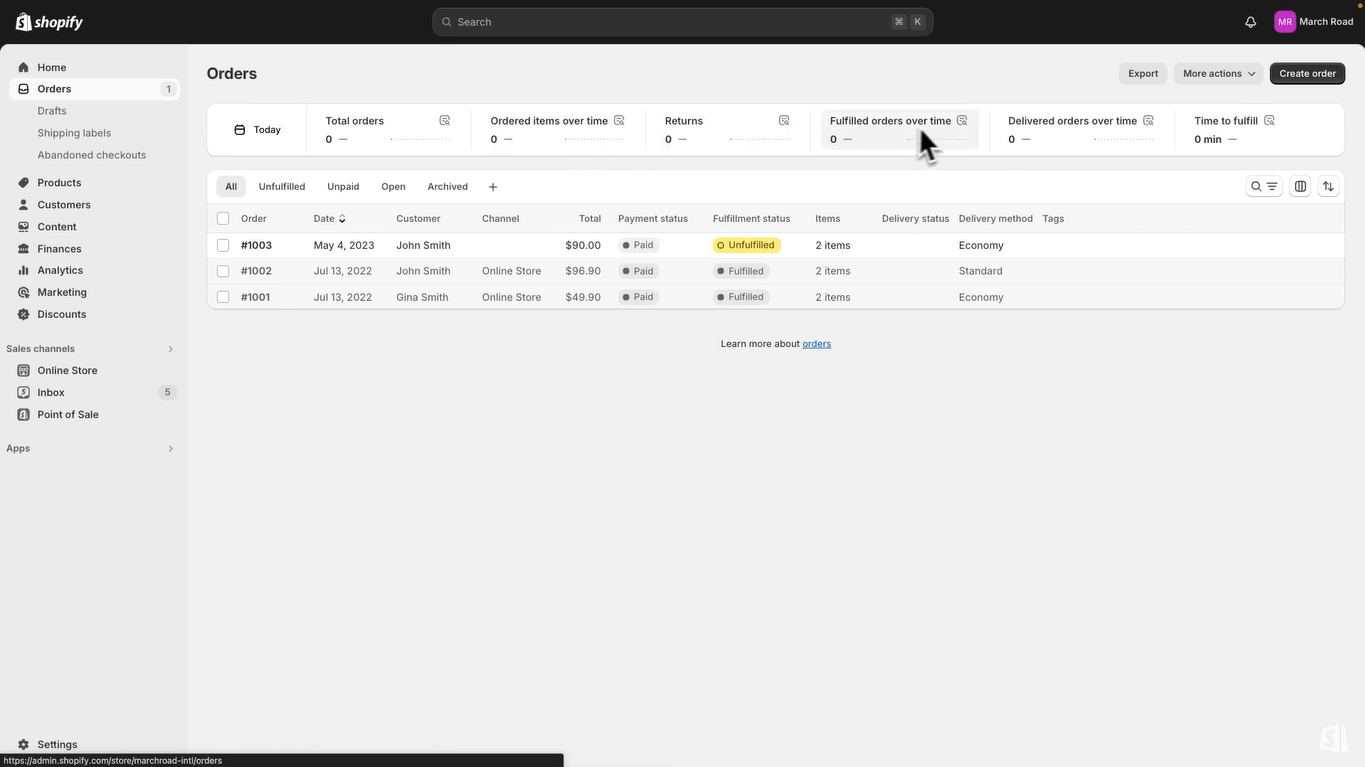
\includegraphics[width=1\textwidth]{frontmatter/assets/backoffice/ch2/shopify_admin.png}
\caption{Interface de gestão de encomendas do Shopify Admin \cite{ShopifyAbout}}
\label{fig:shopify_admin}
\end{figure}

\paragraph{Contributos para o projeto}
\begin{itemize}
  \item Separação clara entre áreas funcionais e ações sensíveis.
  \item Utilização de perfis e permissões para limitar operações por tipo de utilizador interno.
  \item Organização de listagens, filtros e vistas de detalhe para tarefas recorrentes.
\end{itemize}

\paragraph{Limitações}
\begin{itemize}
  \item Domínio fortemente orientado a comércio eletrónico, sem correspondência direta com todos os fluxos do painel desenvolvido.
  \item Produto fechado, sem acesso à arquitetura interna ou possibilidade de reutilização estrutural.
  \item Informação pública limitada sobre auditoria detalhada de ações de operadores.
\end{itemize}

\subsection{Stripe Dashboard}
\label{subsec:stripe_dashboard}

O Stripe Dashboard é o painel de administração da Stripe para acompanhamento de pagamentos, disputas, reembolsos, eventos e membros de equipa. É uma referência relevante para operações financeiras, porque apresenta informação sensível com histórico, filtros e detalhe suficiente para apoiar decisões operacionais.

A documentação da Stripe descreve a atribuição de funções a membros da equipa, a possibilidade de um utilizador acumular vários papéis e a existência de histórico de segurança com atividade dos membros da conta \cite{StripeTeams}. As funções específicas do Stripe Identity, como \textit{Identity Analyst} e \textit{Identity View Only}, mostram uma separação operacional entre consulta e revisão de verificações de identidade \cite{StripeUserRoles}. A Figura~\ref{fig:stripe_dashboard} ilustra uma vista de gestão de transações, relevante para compreender como um painel financeiro apresenta estados, valores e ações associadas.

\begin{figure}[H]
\centering
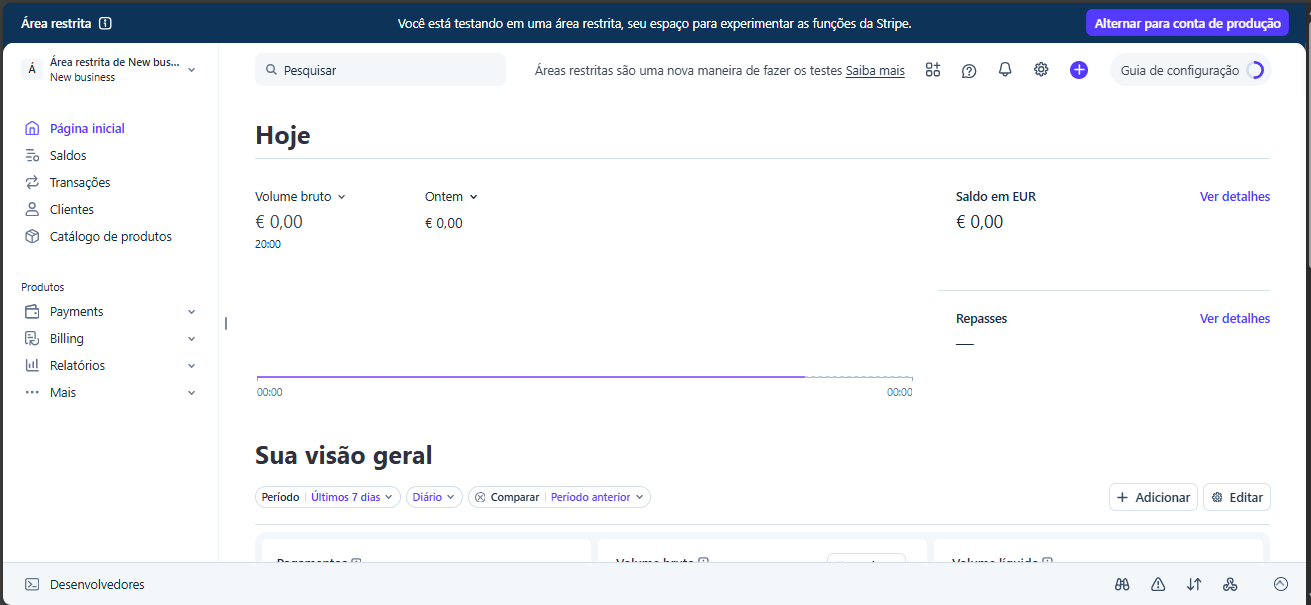
\includegraphics[width=1\textwidth]{frontmatter/assets/backoffice/ch2/stripe_dashboard.png}
\caption{Interface de gestão de transações do Stripe Dashboard \cite{StripeDashboard}}
\label{fig:stripe_dashboard}
\end{figure}

\paragraph{Contributos para o projeto}
\begin{itemize}
  \item Separação de permissões por tipo de operação financeira.
  \item Histórico de atividade associado a membros da conta.
  \item Apresentação de transações com estados, filtros e detalhe operacional.
\end{itemize}

\paragraph{Limitações}
\begin{itemize}
  \item Foco específico no domínio financeiro, sem cobertura de outros fluxos administrativos.
  \item Produto fechado, não adaptável a regras de negócio externas.
  \item A documentação pública descreve conceitos de utilização, mas não a implementação interna do painel.
\end{itemize}

\subsection{Directus}
\label{subsec:directus}

O Directus representa uma abordagem orientada a dados. A ferramenta disponibiliza uma interface de administração sobre bases de dados existentes e permite definir permissões por coleção, ação, campo e política \cite{DirectusPermissions}. Esta granularidade torna o Directus relevante para sistemas em que a principal necessidade é consultar e alterar entidades persistidas.

A Figura~\ref{fig:directus} apresenta uma interface de gestão de dados do Directus. A estrutura evidencia uma lógica comum em ferramentas deste tipo: o modelo de dados serve de base à interface, e a administração é organizada em torno de coleções, campos e operações.

\begin{figure}[H]
\centering
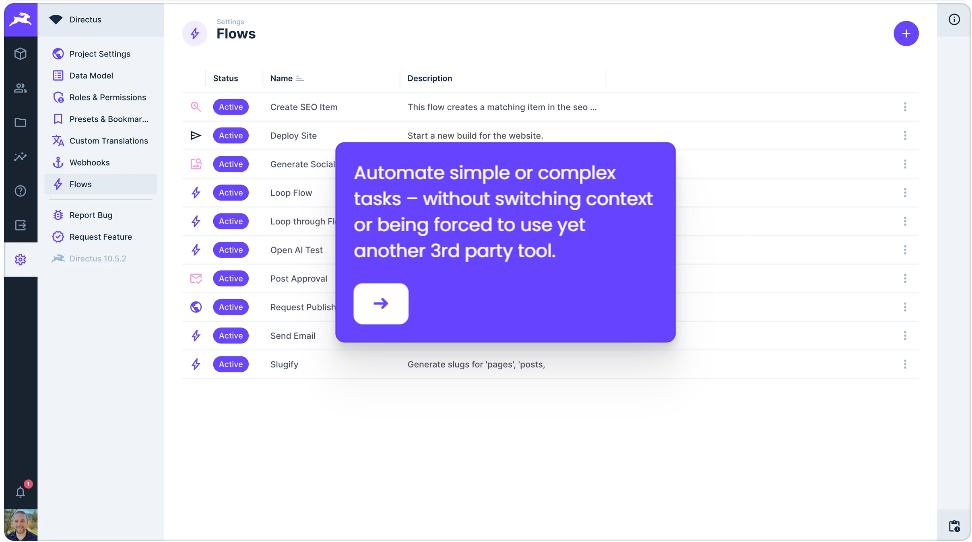
\includegraphics[width=1\textwidth]{frontmatter/assets/backoffice/ch2/directus.png}
\caption{Interface de gestão de dados do Directus \cite{DirectusAbout}}
\label{fig:directus}
\end{figure}

\paragraph{Contributos para o projeto}
\begin{itemize}
  \item Permissões granulares por entidade, campo e ação.
  \item Administração rápida de dados existentes sem desenvolver todas as vistas manualmente.
  \item Registo de atividade e configuração centralizada de regras de acesso.
\end{itemize}

\paragraph{Limitações}
\begin{itemize}
  \item Interface construída a partir do modelo de dados, menos adequada a fluxos de negócio com estados e validações próprias.
  \item Necessidade de configuração ou desenvolvimento adicional para processos de aprovação específicos.
  \item Dependência da forma como as entidades estão modeladas na base de dados.
\end{itemize}

\subsection{Appsmith}
\label{subsec:appsmith}

O Appsmith segue uma abordagem \textit{low-code} para criação de ferramentas internas. A documentação descreve a ligação a bases de dados e \glspl{API}, a construção de interfaces com componentes visuais e a escrita de lógica através de consultas e JavaScript \cite{AppsmithDocs}. Esta solução é relevante porque mostra uma alternativa à criação manual de um painel completo, sobretudo em contextos de prototipagem ou de ferramentas internas de baixa complexidade.

A Figura~\ref{fig:appsmith} mostra a construção visual de uma ferramenta interna no Appsmith, com componentes de interface ligados a fontes de dados. Esta abordagem reduz o tempo inicial de desenvolvimento, mas desloca parte da lógica para configurações e scripts dentro da própria ferramenta.

\begin{figure}[H]
\centering
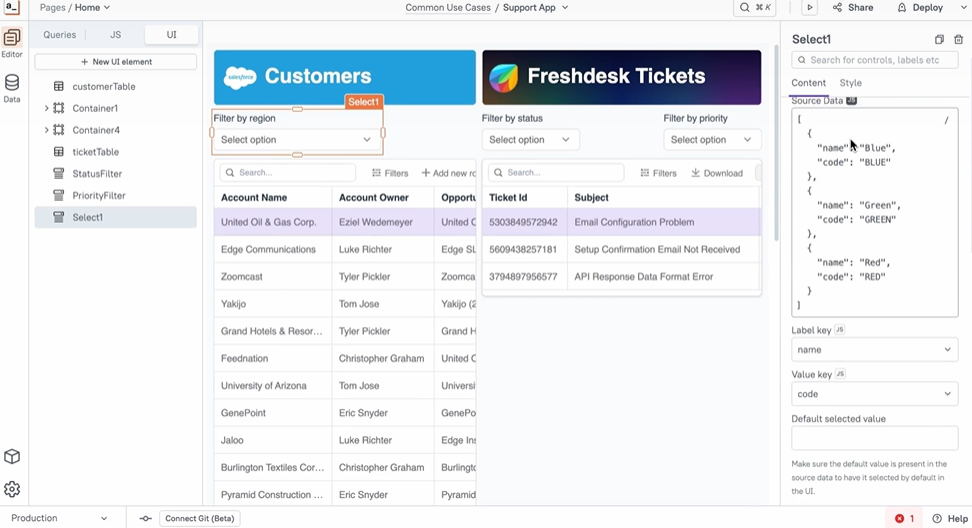
\includegraphics[width=1\textwidth]{frontmatter/assets/backoffice/ch2/appsmith.png}
\caption{Interface de construção de ferramentas internas no Appsmith \cite{AppsmithAbout}}
\label{fig:appsmith}
\end{figure}

\paragraph{Contributos para o projeto}
\begin{itemize}
  \item Criação rápida de interfaces internas ligadas a dados e \glspl{API}.
  \item Adequação a protótipos e painéis operacionais de baixa complexidade.
  \item Redução do esforço inicial em formulários, tabelas e ligações a fontes de dados.
\end{itemize}

\paragraph{Limitações}
\begin{itemize}
  \item Lógica de negócio distribuída por componentes e scripts, com impacto na testabilidade.
  \item Menor controlo sobre a arquitetura da aplicação quando comparado com uma implementação própria.
  \item Adequação limitada a fluxos sensíveis que exigem auditoria consistente e validação transversal no servidor.
\end{itemize}

\subsection{Análise comparativa}
\label{subsec:analise_comparativa_backoffices}

A Tabela~\ref{tab:comparacao_abordagens_backoffice} sintetiza os exemplos analisados e a sua relevância para o projeto, usando a abordagem apenas como uma característica de enquadramento.

\begin{table}[H]
\caption{Comparação de exemplos de painéis de administração}
\label{tab:comparacao_abordagens_backoffice}
\begin{center}
\footnotesize
\begin{tabular}{|p{2.5cm}|p{2.6cm}|p{3.8cm}|p{3.9cm}|}
\hline
\textbf{Exemplo} & \textbf{Abordagem} & \textbf{Contributo observado} & \textbf{Limitação para o projeto} \\ \hline
Shopify Admin & Painel comercial fechado & Organização operacional de áreas funcionais, permissões de equipa, listagens e ações de detalhe. & Produto fechado, orientado a comércio eletrónico e com acesso limitado à implementação interna. \\ \hline
Stripe Dashboard & Painel comercial financeiro & Gestão de operações sensíveis, histórico de segurança, membros da conta e informação financeira com estados. & Produto fechado e centrado no domínio financeiro, sem adaptação direta ao modelo multiaplicação pretendido. \\ \hline
Directus & Administração orientada a dados & Permissões granulares por entidade, campo e ação, com administração rápida de dados existentes. & Menor adequação a fluxos de negócio específicos, processos de aprovação e estados operacionais complexos. \\ \hline
Appsmith & Ferramenta \textit{low-code} & Criação rápida de ferramentas internas ligadas a dados e \glspl{API}. & Lógica de negócio distribuída por componentes e scripts, com impacto na testabilidade e na validação transversal. \\ \hline
Solução adotada & Implementação à medida & Controlo sobre autorização, auditoria, fluxos próprios, integração com a base existente e evolução multiaplicação. & Maior esforço inicial de desenvolvimento e manutenção. \\ \hline
\end{tabular}
\end{center}
\end{table}

Da comparação resulta que nenhum dos exemplos prontos responde integralmente ao conjunto de requisitos do projeto. As soluções comerciais ajudam a identificar padrões, mas não são reutilizáveis. As ferramentas configuráveis aceleram aplicações internas de baixa complexidade, mas perdem adequação quando o domínio exige autorização transversal, auditoria própria, fluxos de decisão específicos e capacidade de acrescentar novas aplicações ao mesmo painel. Assim, a implementação à medida foi a opção mais adequada aos critérios definidos para o contexto da empresa.

%----------------------------------------------------------------------------------------

\section{Princípios técnicos relevantes}
\label{sec:principios_tecnicos_relevantes}

Mais do que comparar tecnologias de forma genérica, o estado da arte deve identificar os princípios que condicionam o desenho de um painel de administração. No projeto desenvolvido, destacam-se três: autorização aplicada de forma consistente, auditoria operacional e separação entre ferramentas genéricas e implementação à medida. Estes princípios são especialmente relevantes num painel multiaplicação, onde permissões e registos de atividade devem manter significado mesmo quando novos domínios funcionais são acrescentados.

\subsection{Autenticação, autorização e separação de responsabilidades}

Num painel de administração, a autenticação confirma a identidade do operador e a autorização determina o que esse operador pode fazer. Esta distinção é importante porque um token de sessão válido não deve, por si só, conceder acesso a todas as áreas internas. Depois do \textit{login}, o sistema precisa de resolver o contexto interno do operador: conta de backoffice, estado da conta, perfis atribuídos, aplicações acessíveis e permissões efetivas.

A interface pode esconder botões ou páginas, mas a decisão final tem de ocorrer no servidor. Caso contrário, bastaria alterar um pedido \gls{HTTP} para tentar executar uma operação não autorizada. Por esse motivo, a OWASP recomenda que os controlos de acesso sejam aplicados no servidor, com uma postura de negação por omissão \cite{OWASPAuthorizationCheatSheet}.

No projeto, esta recomendação traduz-se em duas camadas complementares. O \textit{front-end} usa permissões para orientar a navegação e reduzir ações visíveis ao operador. O \textit{back-end}, por sua vez, valida permissões em cada endpoint sensível. Esta separação evita que a interface seja tratada como fonte de verdade para autorização e permite aplicar o mesmo modelo a diferentes aplicações dentro do \textit{backoffice}.

\subsection{Auditoria operacional}

A auditoria é uma capacidade central em sistemas internos. Para além de registar que uma entidade mudou de estado, o sistema deve identificar quem executou a ação, quando, sobre que entidade e com que resultado. Este requisito ganha importância em operações financeiras, revisão de conteúdo, gestão de utilizadores e configuração de permissões.

O Stripe Dashboard é um exemplo público de painel que expõe histórico de segurança associado à atividade dos membros da conta \cite{StripeTeams}. No projeto JustCauses, a auditoria foi tratada como uma responsabilidade própria do painel, com registos imutáveis em DynamoDB. Esta opção é compatível com a necessidade de escrita frequente e consulta por eventos. O suporte a \textit{Time to Live} do DynamoDB permite ainda gerir a retenção de registos quando existirem políticas de expiração definidas \cite{DynamoDBTTL}.

\subsection{Ferramenta genérica ou implementação à medida}

A adoção de uma ferramenta genérica de administração deve ser avaliada de acordo com o grau de especificidade do domínio. Quando o problema consiste sobretudo em listar, criar, editar e remover entidades, soluções configuráveis podem reduzir o esforço inicial. Quando o domínio exige fluxos de aprovação, permissões configuráveis por aplicação e página, auditoria interna e integração com serviços já existentes, a vantagem inicial dessas ferramentas pode ser anulada pelo custo de adaptação.

No caso deste estágio, a implementação à medida não resulta de rejeição das ferramentas existentes. Resulta da combinação de três fatores: a empresa já possuía uma base de código em React e Node.js; o modelo de permissões tinha requisitos próprios; e o painel precisava de evoluir como parte do ecossistema OnlyHighIQ, não como aplicação administrativa isolada. Esta orientação permite que o módulo transversal de administração do próprio \textit{backoffice} seja reutilizado quando novas aplicações forem adicionadas.

%----------------------------------------------------------------------------------------

\section{Tecnologias enquadradoras do projeto}
\label{sec:tecnologias_enquadradoras}

Algumas tecnologias usadas no projeto não foram escolhidas durante o estágio. React, TypeScript, Node.js, Express, PostgreSQL e \gls{AWS} já faziam parte da base técnica da empresa ou da arquitetura prevista para o ecossistema. Por esse motivo, não faria sentido apresentar uma comparação extensa entre React, Vue e Angular, ou entre Express, FastAPI e Spring Boot, como se a seleção tivesse sido feita de raiz no âmbito deste trabalho.

A decisão relevante foi avaliar se a base existente era adequada para consolidar um painel de administração seguro, evolutivo e preparado para várias aplicações. No \textit{front-end}, React com TypeScript e Vite oferece uma base suficiente para construir interfaces internas com componentes reutilizáveis, rotas protegidas e integração com serviços de autenticação. A menor complexidade visual das páginas torna menos relevante uma comparação profunda entre \textit{frameworks} de interface. O desafio principal não esteve na tecnologia visual, mas na coerência entre navegação, permissões, seleção de aplicação e chamadas à \gls{API}.

No \textit{back-end}, Node.js com Express e TypeScript permite manter a mesma linguagem entre cliente e servidor, simplificando contratos, tipos e integração com bibliotecas do ecossistema \textit{npm}. A persistência relacional em PostgreSQL é adequada para entidades transacionais da plataforma, enquanto o DynamoDB foi usado para dados de configuração e auditoria. Esta separação evita misturar dados operacionais críticos com registos de eventos e configurações administrativas.

A autenticação assenta no AWS Cognito. A documentação do serviço descreve a utilização de grupos em \textit{user pools}, com inclusão dos grupos nos tokens através da \textit{claim} \texttt{cognito:groups} \cite{AWSCognitoGroups}. No entanto, o projeto não depende apenas desses grupos para decidir o acesso. Após o \textit{login}, o sistema obtém o contexto interno do operador, incluindo perfil, aplicação e permissões efetivas. Esta decisão torna o modelo mais flexível do que uma autorização baseada apenas no token de autenticação, pois permite associar o mesmo operador a diferentes aplicações com permissões distintas.

%----------------------------------------------------------------------------------------

\section{Análise e seleção da abordagem}
\label{sec:analise_selecao}

A abordagem adotada no projeto foi manter a base técnica existente e desenvolver o painel à medida. Esta decisão é justificada por quatro motivos principais.

Primeiro, o painel precisava de respeitar a arquitetura já existente da empresa. A introdução de uma ferramenta externa de administração obrigaria a adaptar rotas, serviços, componentes e contratos de \gls{API} a uma abstração que não fazia parte da base existente. O benefício seria maior num projeto iniciado de raiz.

Segundo, o requisito de autorização era transversal. O sistema não precisava apenas de esconder opções na interface; precisava de validar aplicação, página e ação no servidor, mantendo consistência entre o \textit{front-end}, o \textit{back-end} e a configuração administrativa de permissões.

Terceiro, a auditoria era parte do desenho da solução. A rastreabilidade de ações internas e tentativas de acesso negado exigia um modelo próprio, integrado com os serviços e entidades do painel.

Por fim, a solução tinha de ser extensível ao ecossistema da OnlyHighIQ. Um painel à medida permite separar módulos transversais, como autenticação, operadores, perfis, permissões e auditoria, de módulos específicos da JustCauses, como campanhas, categorias, transações e levantamentos. Esta separação evita que a primeira aplicação suportada pelo painel condicione a evolução futura do \textit{backoffice}.

%----------------------------------------------------------------------------------------

\section{Sumário}
\label{sec:sumario_cap2}

A análise realizada mostra que o estado da arte dos painéis de administração deve ser observado sobretudo através de capacidades: controlo de acesso, auditoria, fluxos operacionais, integração com dados, manutenibilidade e evolução multiaplicação. A escassez de exemplos públicos completos não invalida a análise; apenas obriga a combinar documentação oficial, padrões observáveis e ferramentas comparáveis.

Os painéis comerciais, como Shopify Admin e Stripe Dashboard, mostram padrões relevantes de gestão de operadores, permissões e histórico de atividade, mas não são adaptáveis ao domínio do projeto. Ferramentas configuráveis como Directus e Appsmith podem acelerar a criação de ferramentas internas, mas tornam-se menos adequadas quando o domínio exige regras próprias de autorização, auditoria e evolução arquitetural. Neste contexto, a implementação à medida sobre a base React, Node.js, PostgreSQL e AWS já existente foi a opção mais coerente, porque permite tratar a JustCauses como primeira aplicação integrada e não como limite definitivo do \textit{backoffice}. Esta síntese fundamenta as decisões de análise e desenho apresentadas no capítulo seguinte.

\chapter{Análise e Desenho da Solução}
\label{cap:analise_desenho}

Neste capítulo descreve-se o processo de análise e o desenho da solução desenvolvida. Começa-se pelos requisitos, organizados segundo a abordagem \gls{FURPS+}, onde a dimensão \textit{Functionality} agrupa os requisitos funcionais e as restantes dimensões cobrem as propriedades de qualidade não funcionais. Em seguida, apresenta-se a análise do domínio que a solução tem de suportar, incluindo o modelo de aplicação e o modelo de domínio. A arquitetura é depois descrita com recurso à abordagem C4+1, combinando os níveis principais do modelo C4 \cite{C4Model} com uma vista física da infraestrutura. Por fim, apresentam-se o modelo de dados administrativo e o modelo de permissões que sustentam a autorização multiaplicação.

%----------------------------------------------------------------------------------------

\section{Requisitos}
\label{sec:requisitos}

Os requisitos da solução foram levantados a partir da especificação interna da empresa \cite{BackofficeSpec} e das discussões realizadas durante a fase de integração com a equipa. Para os organizar, adotou-se a abordagem \gls{FURPS+}, que classifica os requisitos de software em cinco dimensões principais, acrescentando ainda restrições adicionais de desenho, implementação ou operação \cite{Rashid2024FURPSMoSCoW}:

\begin{itemize}
  \item \textit{Functionality}: capacidades funcionais que o sistema deve disponibilizar.
  \item \textit{Usability}: aspetos da interface que afetam a utilização por operadores internos.
  \item \textit{Reliability}: capacidade de manter integridade, disponibilidade e comportamento previsível perante falhas ou operações inválidas.
  \item \textit{Performance}: tempos de resposta, carregamento inicial e impacto das operações sobre os recursos do sistema.
  \item \textit{Supportability}: manutenibilidade, testabilidade, modularidade e capacidade de adaptação da solução.
\end{itemize}

\noindent\textbf{Functionality}

Em vez de detalhar cada fluxo operacional isoladamente, os requisitos funcionais privilegiam aquilo que o sistema precisa de garantir para ser seguro, utilizável e evolutivo no contexto do ecossistema OnlyHighIQ. A organização seguinte relaciona-os com os objetivos definidos na introdução, usando o objetivo principal (OP) e os objetivos específicos OE1.1 a OE1.5 e OE2.1 a OE2.5.

\medskip\noindent\textit{Autenticação, autorização e administração}: este grupo concretiza sobretudo os objetivos OE1.1, OE1.2 e OE1.3, porque define a base comum de identidade, autorização e gestão de operadores reutilizável por várias aplicações.

\begin{itemize}
  \item \textbf{RF01}: o painel deve autenticar operadores internos através do AWS Cognito, com gestão de sessão e suporte a \gls{MFA}.
  \item \textbf{RF02}: após a autenticação, o sistema deve resolver o contexto interno do operador, incluindo perfis atribuídos, aplicações acessíveis e permissões efetivas.
  \item \textbf{RF03}: o acesso ao backoffice de gestão e ao painel operacional da JustCauses deve ser separado por aplicação, impedindo a entrada em áreas não autorizadas.
  \item \textbf{RF04}: o sistema deve controlar o acesso a páginas com base em guardas de rota e em regras configuráveis por página.
  \item \textbf{RF05}: as permissões exigidas por cada página devem poder ser alteradas sem nova publicação da aplicação.
  \item \textbf{RF06}: todos os endpoints sensíveis da \gls{API} devem validar permissões no servidor antes de executar qualquer operação.
  \item \textbf{RF07}: o painel deve disponibilizar mecanismos de gestão administrativa para contas internas, perfis de acesso, permissões por aplicação e configuração do modelo de autorização.
\end{itemize}

\medskip\noindent\textit{Operação da plataforma}: este grupo concretiza sobretudo os objetivos OE2.1 a OE2.5, aplicando a estrutura comum à primeira aplicação integrada no ecossistema.

\begin{itemize}
  \item \textbf{RF08}: o painel deve disponibilizar um \textit{dashboard} com métricas operacionais relevantes e indicadores de atividade da plataforma.
  \item \textbf{RF09}: o painel deve suportar a revisão do ciclo de vida das campanhas, incluindo estados de aprovação, rejeição e pedido de alterações.
  \item \textbf{RF10}: o painel deve permitir criar, editar e desativar categorias de campanhas.
  \item \textbf{RF11}: o painel deve suportar a verificação \gls{KYC} de utilizadores individuais e a verificação \gls{KYB} de organizações, incluindo consulta de dados submetidos, decisão administrativa, notificação e auditoria.
  \item \textbf{RF12}: a arquitetura deve permitir incorporar outros fluxos operacionais do ecossistema sem alterar o núcleo do mecanismo de autorização.
\end{itemize}

\medskip\noindent\textit{Rastreabilidade}: este grupo apoia simultaneamente o OP e o OE1.4, uma vez que a auditoria é uma capacidade transversal necessária para administrar aplicações internas com responsabilização.

\begin{itemize}
  \item \textbf{RF13}: o painel deve manter um registo imutável das ações relevantes e das tentativas de acesso negado, consultável por filtros de data, operador e tipo de evento.
\end{itemize}

A Tabela~\ref{tab:mapeamento_objetivos_requisitos} resume a relação entre objetivos e requisitos.

\begin{table}[H]
\caption{Relação entre objetivos e requisitos}
\label{tab:mapeamento_objetivos_requisitos}
\begin{center}
\small
\begin{tabular}{|p{2.2cm}|p{5.2cm}|p{5.4cm}|}
\hline
\textbf{Objetivo} & \textbf{Foco} & \textbf{Requisitos associados} \\ \hline
OP & Base comum de backoffice multiaplicação & RF01 a RF13 e RNF01 a RNF16 \\ \hline
OE1.1 & Autenticação e contexto administrativo do operador & RF01, RF02, RNF04 \\ \hline
OE1.2 & Perfis e permissões por aplicação & RF03, RF07, RNF05, RNF14 \\ \hline
OE1.3 & Controlo de acesso em aplicação, página, interface e \gls{API} & RF04, RF05, RF06, RNF12 \\ \hline
OE1.4 & Auditoria, acessos negados e atividade dos operadores & RF13, RNF06, RNF10 \\ \hline
OE1.5 & Arquitetura e persistência extensíveis & RF12, RNF11, RNF13, RNF14, RNF15, RNF16 \\ \hline
OE2.1 & Integração da JustCauses como primeira aplicação operacional & RF03, RF08, RF12 \\ \hline
OE2.2 & Revisão de campanhas e notificação associada & RF09, RF13 \\ \hline
OE2.3 & Gestão de categorias e dados operacionais & RF10 \\ \hline
OE2.4 & Dashboard, analytics e indicadores operacionais & RF08 \\ \hline
OE2.5 & Verificação de identidade e oficialidade & RF11, RF13 \\ \hline
\end{tabular}
\end{center}
\end{table}

\noindent\textbf{Usability}
\begin{itemize}
  \item \textbf{RNF01}: a interface deve ser utilizável por operadores sem formação técnica, com navegação clara entre módulos e separação visível entre aplicações.
  \item \textbf{RNF02}: ações indisponíveis para o operador devem ser omitidas ou bloqueadas de forma explícita, para que a interface não sugira operações não autorizadas.
  \item \textbf{RNF03}: operações críticas devem apresentar mensagens claras de confirmação, erro ou acesso negado.
\end{itemize}

\noindent\textbf{Reliability}
\begin{itemize}
  \item \textbf{RNF04}: toda a comunicação deve ser feita sobre HTTPS, com autenticação obrigatória nos pontos de entrada do painel e suporte a \gls{MFA} via AWS Cognito.
  \item \textbf{RNF05}: as validações de servidor devem rejeitar operações que violem o modelo de autorização, incluindo permissões associadas à aplicação errada ou múltiplos perfis da mesma aplicação.
  \item \textbf{RNF06}: os registos de auditoria devem ser imutáveis e associados a exatamente um operador interno, evitando registos anónimos no contexto administrativo.
  \item \textbf{RNF07}: o sistema deve utilizar os mecanismos de disponibilidade e monitorização da infraestrutura AWS, nomeadamente CloudWatch para observabilidade.
\end{itemize}

\noindent\textbf{Performance}
\begin{itemize}
  \item \textbf{RNF08}: as respostas da \gls{API} para operações de leitura devem ter uma latência inferior a 500 ms em condições normais.
  \item \textbf{RNF09}: o carregamento inicial do painel deve ocorrer em menos de 3 segundos em condições normais de utilização.
  \item \textbf{RNF10}: o módulo de auditoria deve absorver picos de escrita sem degradar o desempenho da base relacional usada pelos dados operacionais da JustCauses.
\end{itemize}

\noindent\textbf{Supportability}
\begin{itemize}
  \item \textbf{RNF11}: o código deve manter separação clara entre interface, rotas, controladores, serviços, repositórios e configuração de infraestrutura.
  \item \textbf{RNF12}: a configuração de \textit{page gates}, isto é, regras de acesso por página, deve poder ser alterada sem nova publicação da aplicação, permitindo adaptar acessos por aplicação e por página.
  \item \textbf{RNF13}: a solução deve manter contratos de \gls{API} estáveis e identificadores de interface adequados à validação manual e aos testes de qualidade existentes.
\end{itemize}

\noindent\textbf{+ Escalabilidade e restrições}
\begin{itemize}
  \item \textbf{RNF14}: o modelo de autorização deve permitir acrescentar futuras aplicações sem redesenhar o núcleo do backoffice, recorrendo a perfis e permissões associados a cada aplicação.
  \item \textbf{RNF15}: operadores, perfis, permissões, \textit{page gates} e auditoria devem permanecer separados dos dados transacionais da JustCauses.
  \item \textbf{RNF16}: a solução deve respeitar a base tecnológica definida pela empresa, incluindo React, Node.js/Express, AWS Cognito, S3, SES, CloudWatch, PostgreSQL, DynamoDB e o processo de entrega com \gls{CI/CD}.
\end{itemize}

%----------------------------------------------------------------------------------------

\section{Análise}
\label{sec:analise_dominio}

O painel de administração opera sobre dois níveis de domínio. O primeiro corresponde aos conceitos transversais do próprio backoffice, como operador interno, aplicação, perfil de acesso, permissão e registo de auditoria. O segundo corresponde ao domínio operacional da JustCauses, que é a primeira aplicação integrada no sistema. Esta distinção é importante porque o relatório não descreve apenas um painel isolado da JustCauses: descreve uma base de administração multiaplicação, onde a JustCauses é o primeiro caso operacional completo.

\subsection{Modelo de aplicação}
\label{subsec:modelo_aplicacao}

O modelo de aplicação traduz os conceitos de domínio que a arquitetura precisa de suportar. No estado atual existem duas áreas funcionais: o backoffice transversal, usado para administração interna, e a JustCauses, primeira aplicação operacional integrada. A Tabela~\ref{tab:entidades_dominio} apresenta as principais entidades e o seu papel.

\begin{table}[H]
\caption{Principais entidades do modelo de aplicação}
\label{tab:entidades_dominio}
\begin{center}
\footnotesize
\begin{tabular}{|l|p{9cm}|}
\hline
\textbf{Entidade} & \textbf{Descrição} \\ \hline
Aplicação         & Área funcional administrada pelo backoffice. No estado atual, existem o backoffice transversal e a aplicação JustCauses, estando o modelo preparado para futuras aplicações. \\ \hline
Operador interno  & Utilizador autorizado a aceder ao backoffice, autenticado via Cognito e associado internamente a perfis de acesso. \\ \hline
Perfil de acesso  & Conjunto de permissões associado a uma aplicação. Um operador pode ter, no máximo, um perfil por aplicação, exceto quando tem um perfil global de backoffice. \\ \hline
Permissão         & Capacidade granular que autoriza uma ação ou consulta. Cada permissão pertence a uma aplicação e só pode ser atribuída a perfis dessa aplicação. \\ \hline
\textit{Page gate} & Configuração que define que permissões permitem abrir uma página do backoffice ou de uma aplicação integrada. \\ \hline
Registo de auditoria & Entrada imutável que documenta uma ação de um operador sobre uma entidade crítica da plataforma, com marca temporal e identificação do responsável. \\ \hline
Utilizador individual & Conta pessoal registada na plataforma JustCauses, com perfil próprio, estado de conta e processo de verificação de identidade associado. \\ \hline
Organização       & Perfil coletivo que pode criar campanhas em nome de uma entidade, com dados de identificação, estado operacional e processo de verificação próprio (\gls{KYB}). \\ \hline
Criador           & Abstração usada para representar quem submete campanhas na JustCauses. Pode corresponder a um utilizador individual ou a uma organização, consoante a natureza do perfil. \\ \hline
Campanha          & Projeto de angariação de fundos submetido por um criador, com ciclo de vida acompanhado pelo painel. \\ \hline
Thread de revisão & Sequência de revisão associada a uma campanha ou alteração submetida, permitindo ao operador aprovar, rejeitar ou pedir correções sem perder o histórico da decisão. \\ \hline
Categoria         & Etiqueta temática associada a campanhas, gerida exclusivamente pelo painel de administração. \\ \hline
Doação            & Contribuição financeira de um utilizador para uma campanha, consultável para acompanhamento operacional. \\ \hline
Depósito          & Entrada financeira no sistema partilhado de pagamentos, usada para acompanhar fundos recebidos antes da sua distribuição operacional. \\ \hline
Transação         & Movimento financeiro registado no sistema, incluindo pagamentos, transferências e outros eventos relevantes para rastreabilidade financeira. \\ \hline
Levantamento      & Pedido de transferência dos fundos angariados por um criador, sujeito a validação e aprovação manual pelo operador. \\ \hline
Verificação KYC   & Processo de validação de identidade de um utilizador individual, comparando dados do perfil com dados de verificação recebidos do fornecedor externo. \\ \hline
Submissão KYB     & Conjunto de documentos e decisão administrativa usados para validar a oficialidade de uma organização e a representação associada. \\ \hline
Documento de verificação & Ficheiro submetido no âmbito de \gls{KYC} ou \gls{KYB}, armazenado externamente e consultado pelo operador quando necessário para a decisão. \\ \hline
Denúncia          & Reporte de conteúdo inadequado submetido por um utilizador para revisão pelo operador do painel. \\ \hline
\end{tabular}
\end{center}
\end{table}

Depois da Tabela~\ref{tab:entidades_dominio}, o aspeto essencial é a separação entre conceitos transversais e conceitos específicos da JustCauses. Aplicação, operador, perfil, permissão, \textit{page gate} e auditoria são reutilizáveis; utilizadores individuais, organizações, criadores, campanhas, threads de revisão, categorias, doações, depósitos, transações, levantamentos e verificações pertencem ao domínio operacional da JustCauses. O conceito de criador evita duplicar regras entre pessoas e organizações: ambos podem submeter campanhas, mas a validação que lhes é aplicável é diferente. Os utilizadores individuais são avaliados por \gls{KYC}; as organizações são avaliadas por \gls{KYB}. Esta distinção também ajuda a perceber porque é que a arquitetura não deve misturar a configuração do backoffice com os dados de negócio de cada aplicação integrada.

A Figura~\ref{fig:domain_model} apresenta esta separação no modelo de domínio usado como referência para o desenho da solução.

\IfFileExists{frontmatter/assets/backoffice/ch3/uml/architecture/domain-model.png}{
\begin{figure}[H]
\centering
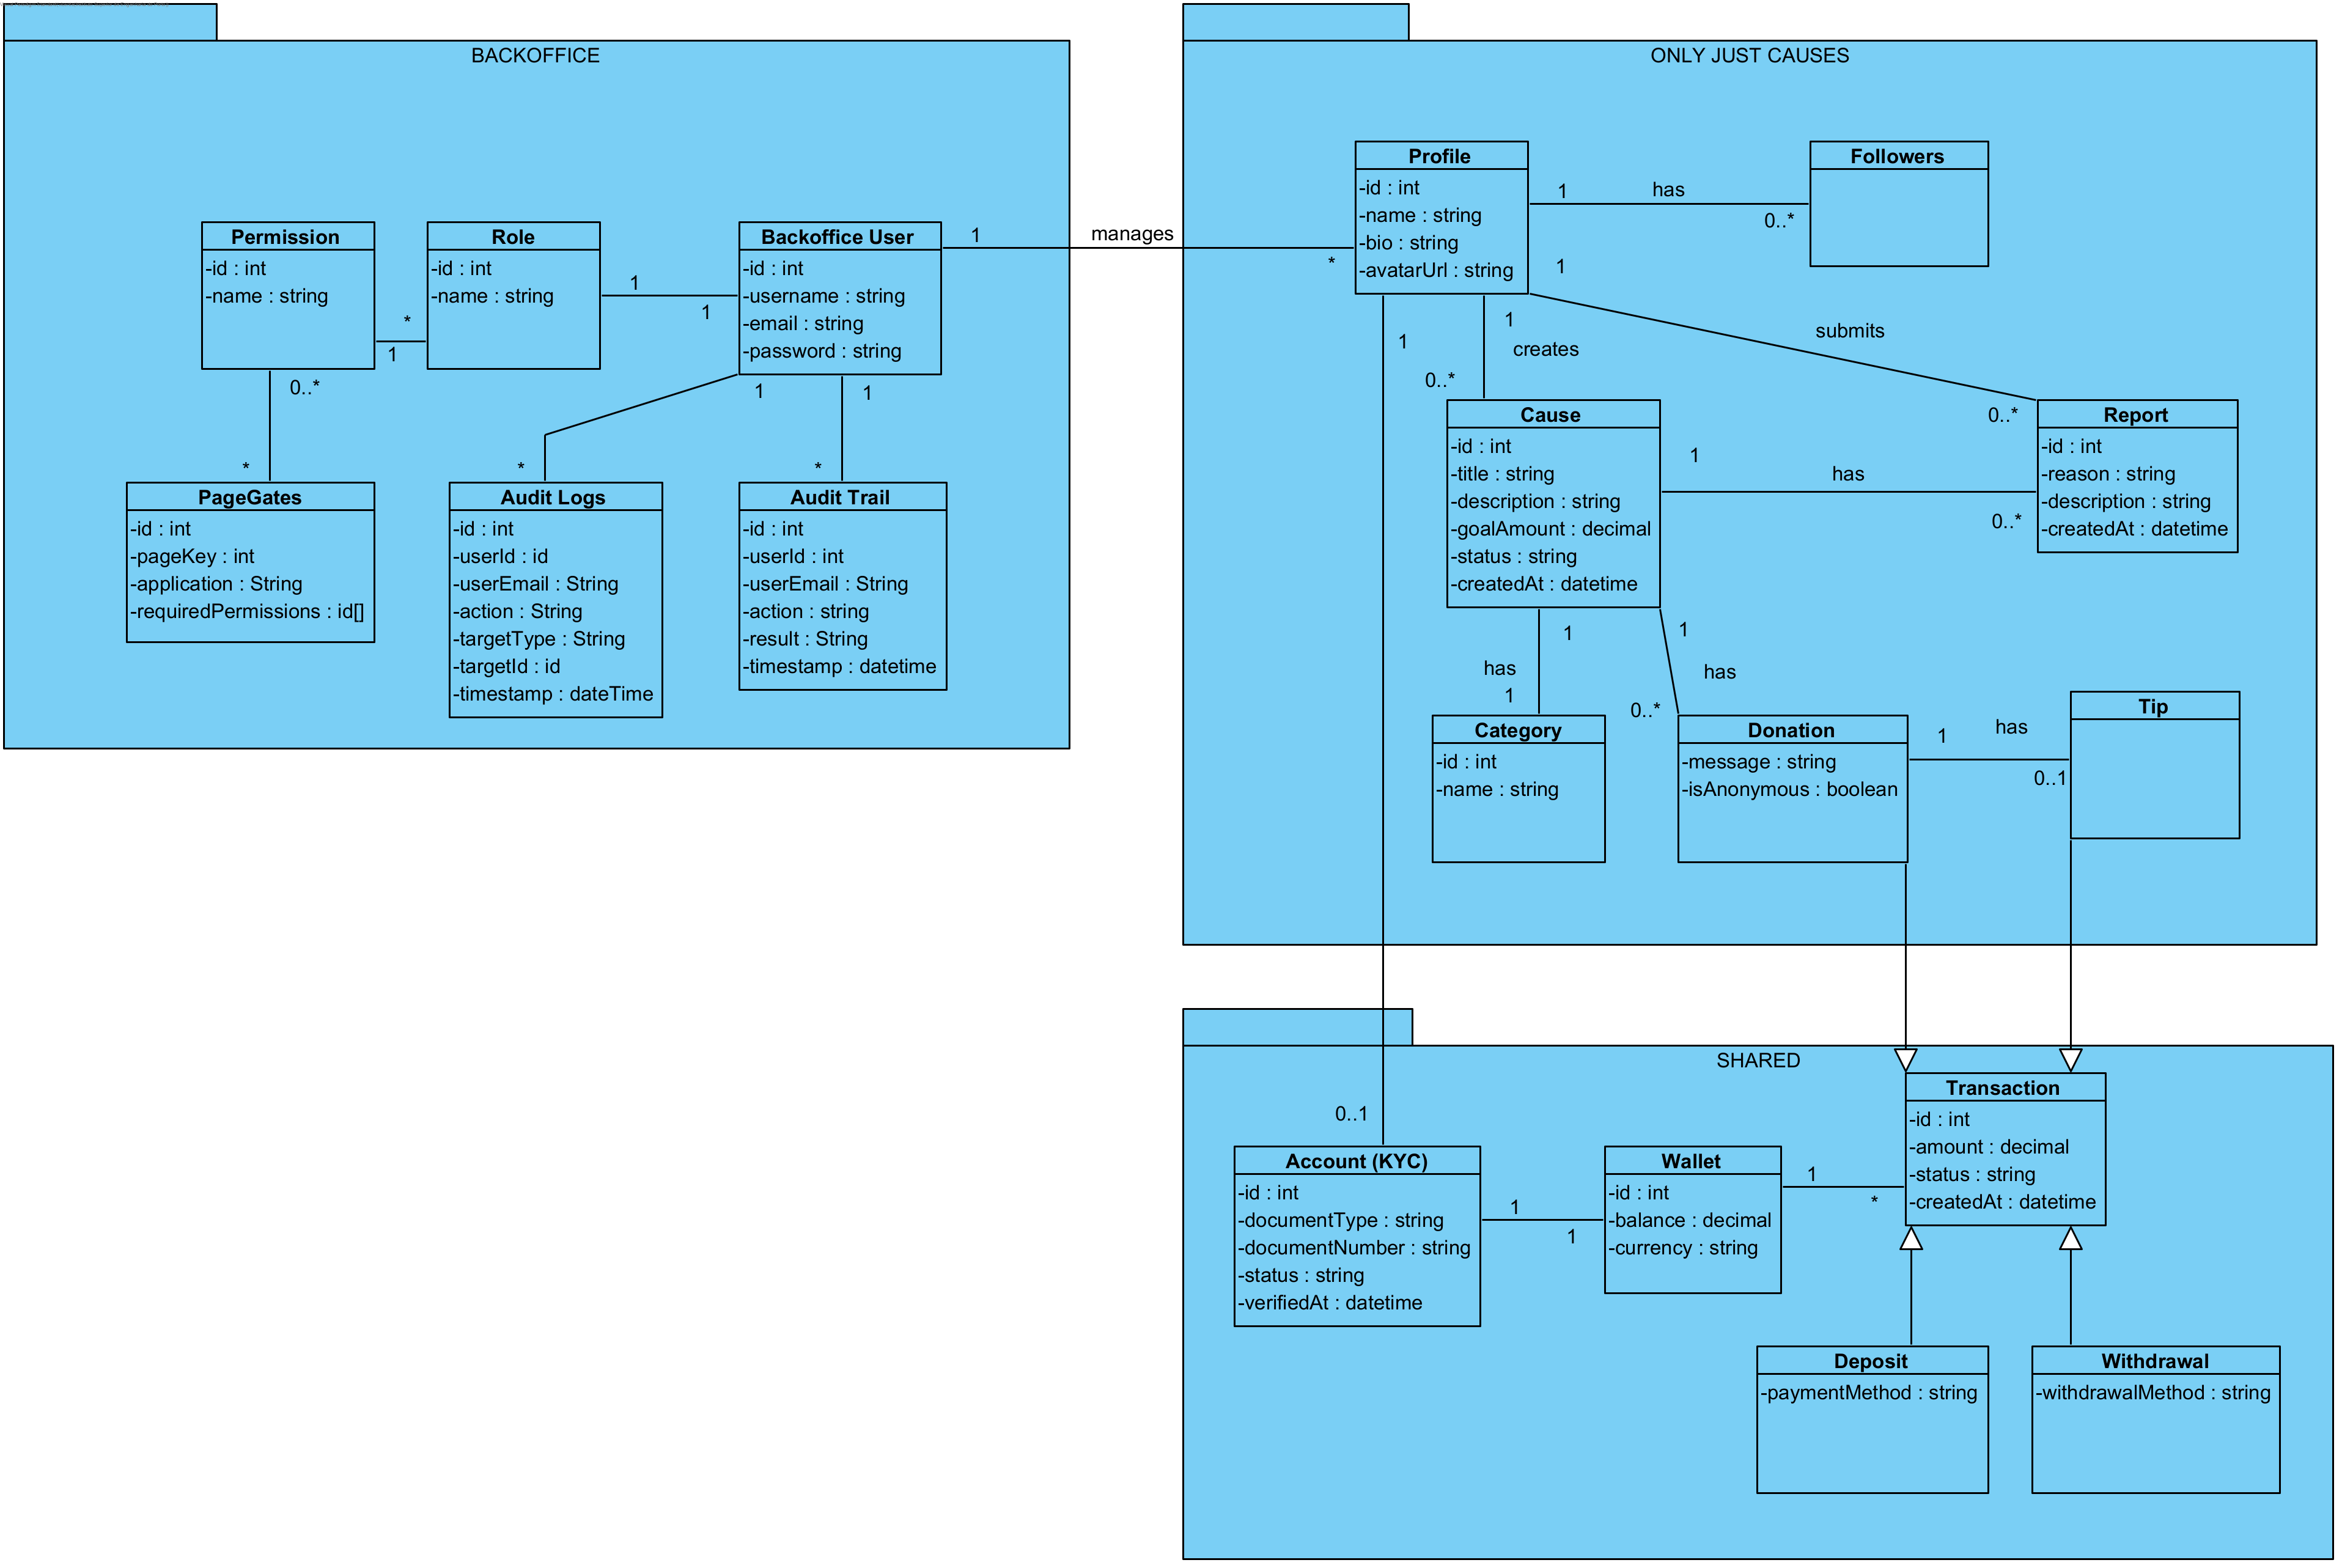
\includegraphics[width=0.95\textwidth, height=0.82\textheight, keepaspectratio]{frontmatter/assets/backoffice/ch3/uml/architecture/domain-model.png}
\caption{Modelo de domínio do backoffice e da JustCauses}
\label{fig:domain_model}
\end{figure}

Depois da Figura~\ref{fig:domain_model}, a leitura pretendida é que o backoffice administra entidades da JustCauses, mas mantém o seu próprio domínio de acesso e auditoria separado. No bloco de backoffice surgem as entidades que suportam autorização e auditoria. No bloco Only Just Causes surgem perfis, organizações, campanhas, categorias, verificações, doações, denúncias e relações de acompanhamento. No bloco partilhado surgem contas, carteiras e movimentos financeiros, incluindo depósitos e levantamentos.
}{}

%----------------------------------------------------------------------------------------

\section{Arquitetura da solução}
\label{sec:arquitetura}

A arquitetura do painel de administração foi definida com base nos requisitos levantados e nas restrições de infraestrutura já existentes no ecossistema da OnlyHighIQ. Para a descrever de forma estruturada, adotou-se uma abordagem C4+1: os níveis C4 principais \cite{C4Model}, que organizam a descrição em contexto do sistema, contentores e componentes, são complementados por uma vista física da infraestrutura. Esta extensão é útil porque o comportamento do backoffice depende também da forma como autenticação, distribuição, computação, persistência e observabilidade estão implantadas na AWS.

\subsection{Nível 1: contexto do sistema}

O painel de administração é um sistema de uso exclusivamente interno, acedido por operadores autorizados da OnlyHighIQ através de um navegador \textit{web}. No nível de contexto, a dependência externa mais relevante para a entrada no sistema é o AWS Cognito, responsável pela autenticação dos operadores. As restantes dependências, como bases de dados, serviços de armazenamento, e-mail transacional e observabilidade, são detalhadas nos níveis seguintes da arquitetura.

A Figura~\ref{fig:c4_level1} mostra o backoffice como sistema interno acedido pela interface de utilizador e integrado com o AWS Cognito para autenticação.

\begin{figure}[H]
\centering
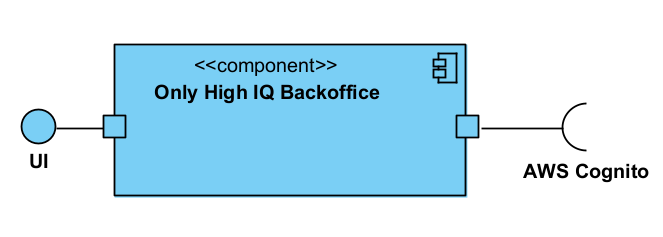
\includegraphics[width=0.95\textwidth, height=0.85\textheight, keepaspectratio]{frontmatter/assets/backoffice/docs/C4-Level1.png}
\caption{Diagrama de contexto: C4 Nível 1}
\label{fig:c4_level1}
\end{figure}

Depois da Figura~\ref{fig:c4_level1}, o ponto a reter é que o backoffice se posiciona como aplicação administrativa interna. O operador não comunica diretamente com os dados da JustCauses ou com serviços de suporte: entra primeiro no painel, autentica-se através do Cognito e só depois executa operações sujeitas ao modelo de autorização descrito nas secções seguintes.

\subsection{Nível 2: contentores e vista física}

O sistema é composto por dois contentores principais: a aplicação \textit{front-end}, desenvolvida em React 19 com TypeScript e Vite, e a \gls{API} \textit{back-end}, desenvolvida em Node.js com Express 5 e TypeScript. A comunicação entre os dois é feita exclusivamente via \gls{REST} sobre HTTPS, com autenticação baseada em tokens JWT emitidos pelo AWS Cognito e validados pelo \textit{back-end} em cada pedido.

A Figura~\ref{fig:c4_level2} evidencia a separação entre interface, \gls{API}, bases de dados e serviços externos. O ponto a reter deste nível é que o \textit{front-end} consome a \gls{API}; não acede diretamente às bases de dados nem decide sozinho autorizações sensíveis.

\begin{figure}[H]
\centering

\includegraphics[width=0.95\textwidth, height=0.85\textheight, keepaspectratio]{frontmatter/assets/backoffice/docs/C4-Level2.png}
\caption{Diagrama de contentores: C4 Nível 2}
\label{fig:c4_level2}
\end{figure}

Depois da Figura~\ref{fig:c4_level2}, a leitura pretendida é a separação de responsabilidades. O navegador apresenta a interface e envia pedidos autenticados; a \gls{API} concentra a validação de tokens, permissões e regras de negócio; o DynamoDB guarda a configuração e a auditoria próprias do backoffice; e as bases Aurora PostgreSQL mantêm os dados operacionais da JustCauses e os dados partilhados do ecossistema. Esta opção suporta uma arquitetura multiaplicação sem criar um backoffice isolado para cada produto.

A camada de persistência é composta por três áreas com responsabilidades distintas: a base Aurora PostgreSQL da JustCauses para dados operacionais da aplicação, a base Aurora PostgreSQL partilhada para entidades comuns do ecossistema, e o AWS DynamoDB para os dados de configuração e rastreabilidade do painel (perfis, permissões, configuração de acesso por rota e registos de auditoria). O acesso a ficheiros, como documentos de \gls{KYC}, documentos de \gls{KYB} e imagens de campanhas, é feito via AWS S3.

\subsubsection{Vista física}
\label{subsec:vista_fisica}

A infraestrutura do painel de administração reside integralmente na \gls{AWS} e usa o conjunto de serviços geridos já adotado pelo ecossistema da \textit{OnlyHighIQ}. A Figura~\ref{fig:vista_fisica} apresenta a vista física da solução, desde a filtragem de tráfego por \gls{WAF} e a distribuição via CloudFront, passando pela autenticação com Cognito, até à execução do \textit{back-end} em instâncias Spot com Auto Scaling distribuídas por três zonas de disponibilidade e à persistência em Aurora Multi-AZ e DynamoDB.

\begin{figure}[H]
\centering
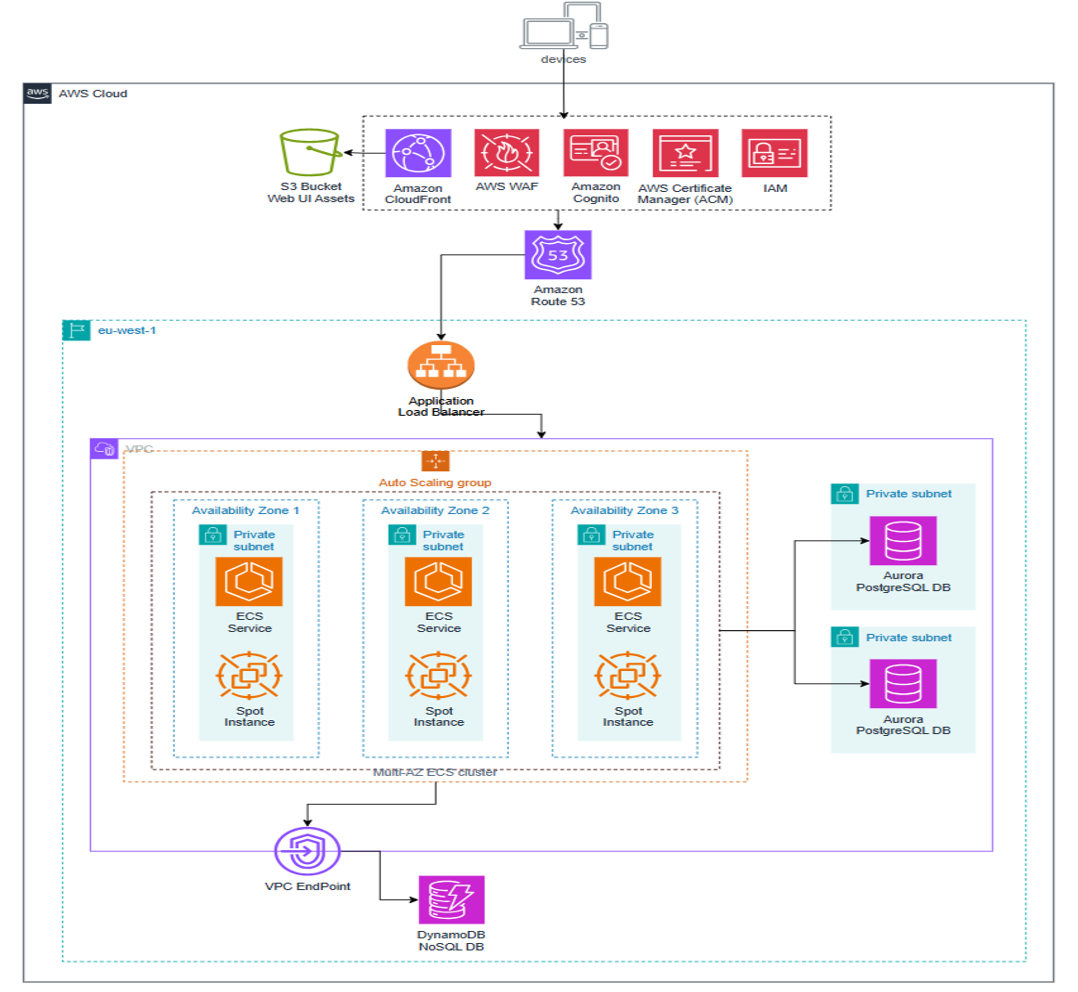
\includegraphics[width=0.95\textwidth, height=0.85\textheight, keepaspectratio]{frontmatter/assets/backoffice/docs/aws-physical-view.png}
\caption{Vista física da infraestrutura AWS do backoffice}
\label{fig:vista_fisica}
\end{figure}

A camada de borda (Route 53, CloudFront com S3, \gls{WAF} e ACM) segue o padrão já estabelecido no ecossistema da \textit{OnlyHighIQ} e não introduz lógica específica do backoffice. O serviço com impacto direto no painel é o Amazon Cognito: gere a identidade dos operadores com \gls{MFA}, emite tokens JWT e organiza utilizadores em grupos que mapeiam para os perfis do painel. O \textit{back-end} valida esses tokens com o \gls{JWKS} público do Cognito sem armazenar credenciais localmente, mantendo a fonte de verdade da identidade fora da aplicação.

Na computação, o servidor Node.js corre em contentores geridos pelo Amazon ECS com instâncias Spot, distribuídos por um grupo de Auto Scaling em três zonas de disponibilidade, combinando custo reduzido com resiliência a falhas de zona.

Na persistência, o Amazon Aurora PostgreSQL armazena os dados relacionais da JustCauses com replicação Multi-AZ. O Amazon DynamoDB é dedicado exclusivamente aos dados de controlo e rastreabilidade do backoffice: utilizadores internos, perfis, permissões, configuração de page gates e registos de auditoria (\texttt{BO\_Users}, \texttt{BO\_Roles}, \texttt{BO\_Permissions}, \texttt{BO\_PageGates}, \texttt{BO\_Logs}). Este acesso é feito através de um VPC Endpoint privado, sem tráfego pela internet pública. A separação entre os dados operacionais da JustCauses e os dados administrativos do painel é uma decisão deliberada: garante que auditoria e configuração de acesso não concorrem com as entidades da plataforma. O Amazon SES completa esta camada ao enviar notificações automáticas a criadores em resposta a decisões do painel, como revisões de campanhas ou alterações de estado de conta.

A Tabela~\ref{tab:aws_servicos} resume os serviços utilizados e o papel de cada um na solução.

\begin{table}[H]
\caption{Serviços AWS e respetivo papel na solução}
\label{tab:aws_servicos}
\begin{center}
\footnotesize
\begin{tabular}{|l|p{9cm}|}
\hline
Serviço AWS & Papel na solução \\ \hline
Amazon Route 53       & Resolução de nomes de domínio da aplicação. \\ \hline
Amazon CloudFront     & Distribuição dos conteúdos estáticos do \textit{front-end} com cache global e HTTPS. \\ \hline
AWS WAF               & Filtragem de tráfego malicioso na camada de distribuição, bloqueando pedidos antes de atingirem a infraestrutura interna. \\ \hline
AWS Certificate Manager & Gestão e renovação automática dos certificados TLS associados ao CloudFront e ao ALB. \\ \hline
Amazon S3 (UI)        & Repositório dos \textit{assets} estáticos compilados do \textit{front-end} React. \\ \hline
Amazon S3 (Docs)      & Armazenamento de documentos de \gls{KYC}/\gls{KYB} e ficheiros de campanhas submetidos pelos criadores. \\ \hline
Amazon Cognito        & Gestão de identidade dos operadores internos do painel, incluindo autenticação com MFA, emissão de tokens JWT e grupos de utilizadores para controlo de acesso. \\ \hline
AWS IAM               & Controlo de permissões entre serviços AWS, incluindo as políticas que autorizam o \textit{back-end} a aceder ao S3, DynamoDB, SES e CloudWatch. \\ \hline
Application Load Balancer & Distribuição do tráfego \gls{HTTP} entre as instâncias do \textit{back-end} Node.js nas diferentes zonas de disponibilidade. \\ \hline
Amazon ECS (Spot)     & Alojamento do servidor \textit{back-end} Node.js com Express em contentores geridos com instâncias Spot, distribuídos por um grupo de Auto Scaling em três zonas de disponibilidade da região \texttt{eu-west-1}. \\ \hline
Amazon Aurora PostgreSQL & Bases relacionais usadas pela JustCauses e pelo domínio partilhado do ecossistema, persistindo contas, perfis, campanhas, doações, levantamentos e verificações \gls{KYC}/\gls{KYB}, com replicação Multi-AZ em duas sub-redes privadas. \\ \hline
Amazon DynamoDB       & Persistência dos dados administrativos do backoffice (\texttt{BO\_Users}, \texttt{BO\_Roles}, \texttt{BO\_Permissions}, \texttt{BO\_PageGates}, \texttt{BO\_Logs}), acedida através de um VPC Endpoint privado sem tráfego pela internet pública. \\ \hline
Amazon SES            & Envio de e-mails transacionais automáticos a criadores e utilizadores em resposta a ações do painel, como decisões sobre campanhas, verificações e estado de contas. \\ \hline
Amazon CloudWatch     & Monitorização de métricas de infraestrutura, alertas de erros e análise de logs do \textit{back-end}. \\ \hline
\end{tabular}
\end{center}
\end{table}

O fluxo de uma operação típica percorre os seguintes serviços: o operador acede à interface \textit{web} servida pelo CloudFront a partir dos \textit{assets} em S3; o tráfego é inspecionado e filtrado pelo \gls{WAF} antes de atingir a infraestrutura interna; o \textit{front-end} autentica-se via Cognito e obtém um token JWT; os pedidos \gls{API} são encaminhados pelo Application Load Balancer para o servidor \textit{back-end} em Amazon ECS com instâncias Spot, geridas por um grupo de Auto Scaling distribuído por três zonas de disponibilidade; o servidor valida o token com o \gls{JWKS} público do Cognito, verifica as permissões do operador e executa a operação sobre o Aurora PostgreSQL Multi-AZ; o registo de auditoria é escrito de forma assíncrona no DynamoDB através de um VPC Endpoint privado, sem atravessar a internet pública; e as notificações transacionais relevantes são enviadas via SES.

O envio de e-mails transacionais é centralizado no \textit{back-end}, evitando que o \textit{front-end} conheça credenciais, remetentes ou detalhes do fornecedor externo. Para notificações automáticas da plataforma, o servidor constrói mensagens HTML parametrizadas e invoca o Amazon SES através do \textit{SDK} da AWS. O remetente é configurado por ambiente e o cliente SES usa credenciais explícitas ou as credenciais disponibilizadas pelo ambiente de execução. Como estas mensagens são consequência de uma operação já validada, a falha no envio é registada nos logs do servidor, mas não deve anular a decisão administrativa já persistida.

\subsection{Nível 3: componentes, implementação e dados}

O Nível 3 decompõe os dois contentores identificados no nível anterior em componentes internos e descreve a organização do código, os fluxos de interação com o sistema e as estruturas de persistência e autorização que sustentam o comportamento do painel.

\subsubsection{Componentes do \textit{back-end}}

A \gls{API} \textit{back-end} é organizada em módulos funcionais correspondentes aos domínios operacionais do painel. Cada módulo segue uma estrutura de camadas inspirada em \textit{Domain-Driven Design}: controladores \gls{HTTP} que tratam o pedido e a resposta, serviços de domínio que contêm a lógica de negócio, repositórios que abstraem o acesso à base de dados, e objetos de transferência de dados (\textit{DTOs}) que definem os contratos de comunicação com o exterior. Esta separação garante que a lógica de negócio não fica acoplada nem à camada de comunicação nem à de persistência, facilitando os testes e a evolução independente de cada camada. A Figura~\ref{fig:c4_level3_be} apresenta esta decomposição ao nível dos componentes do servidor.

\begin{figure}[H]
\centering
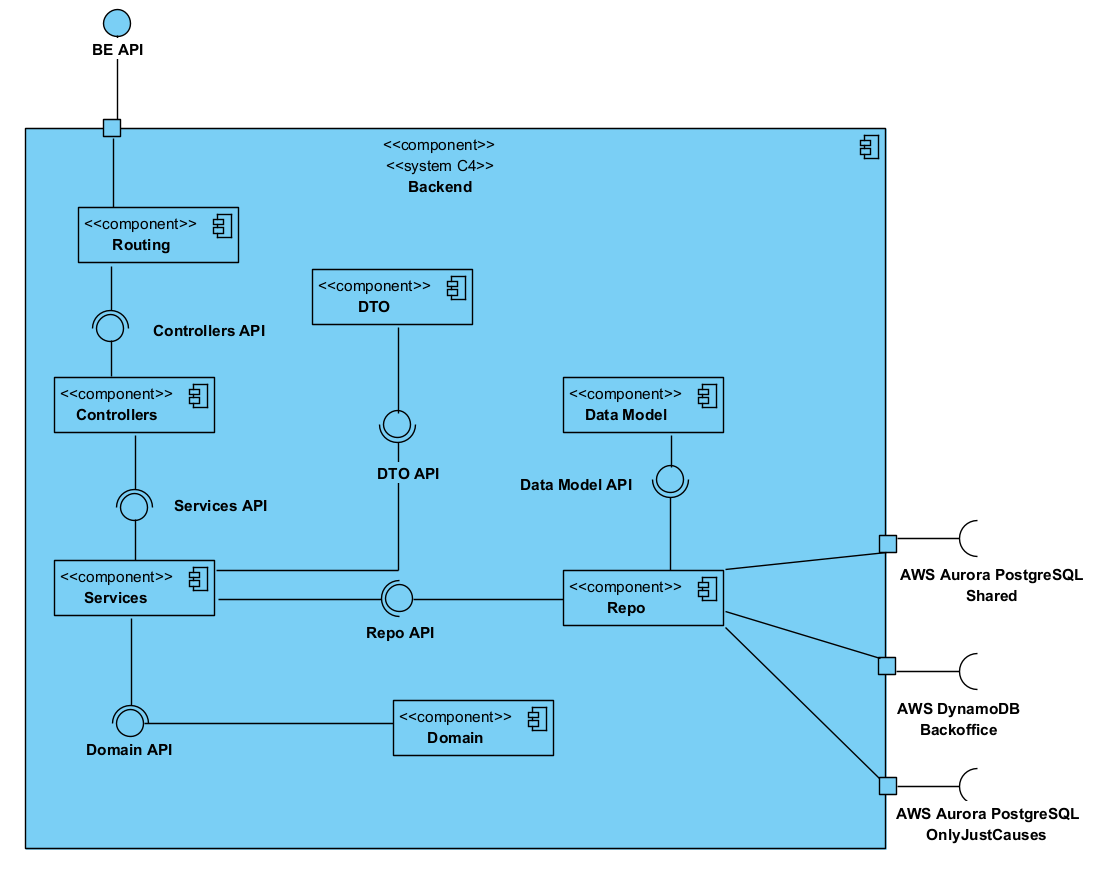
\includegraphics[width=0.95\textwidth, height=0.85\textheight, keepaspectratio]{frontmatter/assets/backoffice/docs/C4-Level3BE.png}
\caption{Diagrama de componentes do \textit{back-end}: C4 Nível 3}
\label{fig:c4_level3_be}
\end{figure}

Depois da Figura~\ref{fig:c4_level3_be}, o ponto a reter é que os módulos não acedem diretamente uns aos outros de forma arbitrária. A autorização entra antes da lógica de negócio, os serviços concentram regras do domínio, os repositórios isolam a persistência e a auditoria acompanha as operações relevantes.

Para além da decomposição por componentes, a implementação do \textit{back-end} seguiu uma separação por camadas. A Figura~\ref{fig:c4_level3_implementation} apresenta essa vista de implementação, centrada na passagem entre rotas, controladores, serviços, repositórios e modelos de domínio. Esta separação reduz o acoplamento entre camadas e permite evoluir módulos sem alterar toda a cadeia de dependências.

\IfFileExists{frontmatter/assets/backoffice/docs/C4-Level3Implementation.png}{
\begin{figure}[H]
\centering
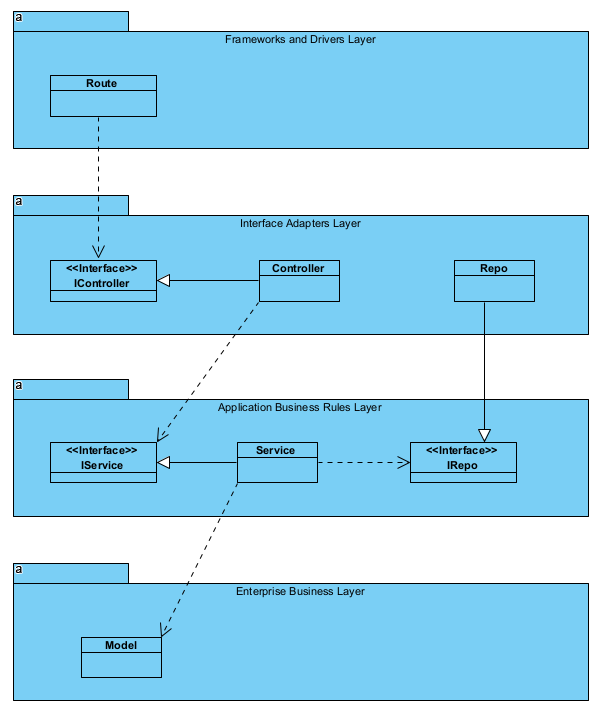
\includegraphics[width=0.9\textwidth, height=0.78\textheight, keepaspectratio]{frontmatter/assets/backoffice/docs/C4-Level3Implementation.png}
\caption{Vista de implementação por camadas}
\label{fig:c4_level3_implementation}
\end{figure}

Depois da Figura~\ref{fig:c4_level3_implementation}, importa perceber a direção das dependências. As rotas pertencem à camada mais externa e encaminham pedidos para controladores. Os controladores adaptam o pedido HTTP para chamadas de serviço. Os serviços concentram as regras de negócio e dependem de interfaces de repositório, não de detalhes concretos de persistência. Os modelos representam os conceitos centrais usados por essas regras. Esta organização ajuda a manter a lógica de negócio protegida de detalhes de infraestrutura.
}{}

\subsubsection{Componentes do \textit{front-end}}

O \textit{front-end} é organizado em páginas e componentes React, com uma camada de serviços responsável pela comunicação com a \gls{API} e uma camada de gestão de estado local. O roteamento é gerido pelo React Router, com proteção de rotas baseada no contexto de acesso devolvido pelo \textit{back-end}: aplicações acessíveis, perfis atribuídos e permissões efetivas. Esta decisão evita que o cliente tenha de reconstruir sozinho regras de autorização a partir do token de autenticação. A Figura~\ref{fig:c4_level3_fe} apresenta esta organização do cliente.

A implementação foi mantida sobre a base React já existente da empresa, em vez de adotar uma ferramenta genérica de administração. Esta decisão preservou o \textit{design system} usado pela OnlyHighIQ e manteve controlo direto sobre fluxos de autorização, auditoria e navegação multiaplicação.

\begin{figure}[H]
\centering
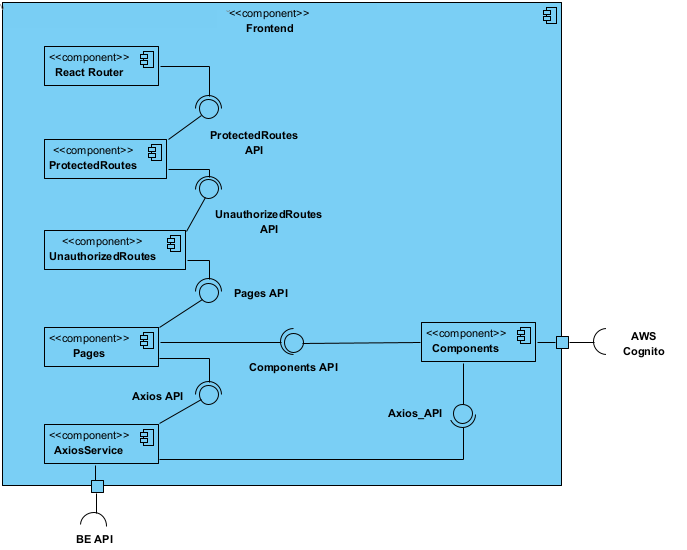
\includegraphics[width=0.95\textwidth, height=0.85\textheight, keepaspectratio]{frontmatter/assets/backoffice/docs/C4-Level3Fe.png}
\caption{Diagrama de componentes do \textit{front-end}: C4 Nível 3}
\label{fig:c4_level3_fe}
\end{figure}

Depois da Figura~\ref{fig:c4_level3_fe}, a leitura pretendida é que a interface não é a fonte final de autorização. O \textit{front-end} melhora a experiência do operador ao esconder páginas e ações indisponíveis, mas trabalha sempre sobre o contexto de acesso calculado no servidor.

\subsubsection{Fluxos de sistema e diagramas de sequência}
\label{sec:diagramas_comportamento}

No Nível 3, os diagramas de componentes explicam a organização interna do \textit{front-end} e do \textit{back-end}. Para completar essa leitura, os \glspl{SSD} seguintes resumem os principais fluxos ao nível da interação entre o operador e o sistema. Os \glspl{SSD} não mostram os componentes internos, mas indicam que pedidos entram no backoffice, que respostas são devolvidas e que decisões do sistema condicionam cada operação. As Figuras~\ref{fig:ssd_login} a~\ref{fig:ssd_kyb_verification} apresentam estes fluxos resumidos; os \glspl{SD} detalhados correspondentes encontram-se no Apêndice~\ref{app:sd_detalhados}, onde cada fluxo é expandido com controladores, serviços, repositórios, persistência e registos de auditoria.

\begin{figure}[H]
\centering

\includegraphics[width=0.9\textwidth, height=0.38\textheight, keepaspectratio]{frontmatter/assets/backoffice/ch3/uml/login-authentication/ssd}
\caption{SSD: autenticação e resolução inicial do operador}
\label{fig:ssd_login}
\end{figure}

Depois da Figura~\ref{fig:ssd_login}, a leitura pretendida é que a autenticação não termina na validação da identidade. O operador inicia a sessão, mas o sistema ainda tem de resolver o utilizador interno, confirmar o estado da conta e calcular o acesso disponível antes de permitir a navegação. O fluxo detalhado encontra-se na Secção~\ref{app:sd_login_full}.

\begin{figure}[H]
\centering

\includegraphics[width=0.9\textwidth, height=0.38\textheight, keepaspectratio]{frontmatter/assets/backoffice/ch3/uml/create-admin-user/ssd}
\caption{SSD: criação de operador administrativo}
\label{fig:ssd_create_admin}
\end{figure}

Depois da Figura~\ref{fig:ssd_create_admin}, a leitura principal é que a criação de operadores administrativos é tratada como uma operação sensível. O sistema valida a autoridade do operador autenticado, cria a conta administrativa, associa o perfil pretendido e regista a ação para auditoria. O detalhe da colaboração interna é apresentado na Secção~\ref{app:sd_create_admin_full}.

\begin{figure}[H]
\centering

\includegraphics[width=0.9\textwidth, height=0.38\textheight, keepaspectratio]{frontmatter/assets/backoffice/ch3/uml/CH4-ROLE-ASSIGNMENT/ssd}
\caption{SSD: atribuição de perfil por aplicação}
\label{fig:ssd_role_assignment}
\end{figure}

Depois da Figura~\ref{fig:ssd_role_assignment}, importa observar que a atribuição de perfis não é uma simples edição de um campo do utilizador. O sistema valida a hierarquia administrativa, a aplicação associada ao perfil, a regra de apenas um perfil por aplicação e a exclusividade dos perfis globais de backoffice. O SD detalhado da Secção~\ref{app:sd_role_assignment_full} mostra onde estas validações são aplicadas.

\begin{figure}[H]
\centering

\includegraphics[width=0.9\textwidth, height=0.38\textheight, keepaspectratio]{frontmatter/assets/backoffice/ch3/uml/roles-permissions/ssd}
\caption{SSD: gestão de perfis e permissões}
\label{fig:ssd_roles_permissions}
\end{figure}

Depois da Figura~\ref{fig:ssd_roles_permissions}, a leitura esperada é que os perfis e permissões são sempre administrados dentro do contexto de uma aplicação. Esta separação impede que permissões de uma aplicação sejam associadas a perfis de outra e suporta a evolução do backoffice para novas aplicações sem alterar o princípio de autorização. A Secção~\ref{app:sd_roles_permissions_full} detalha o carregamento, a edição e a persistência destas alterações.

\begin{figure}[H]
\centering

\includegraphics[width=0.9\textwidth, height=0.38\textheight, keepaspectratio]{frontmatter/assets/backoffice/ch3/uml/CH4-PAGE-GATES/ssd}
\caption{SSD: configuração de page gates}
\label{fig:ssd_page_gates}
\end{figure}

Depois da Figura~\ref{fig:ssd_page_gates}, a leitura principal é que o acesso a páginas é configurável a partir do próprio backoffice. O operador escolhe a aplicação, seleciona a página e define que permissões dão acesso a essa área, enquanto o sistema valida a consistência das permissões e guarda a configuração. O fluxo detalhado é apresentado na Secção~\ref{app:sd_page_gates_full}.

\begin{figure}[H]
\centering

\includegraphics[width=0.9\textwidth, height=0.38\textheight, keepaspectratio]{frontmatter/assets/backoffice/ch3/uml/CH4-USER-ACTIVITY/ssd}
\caption{SSD: consulta de atividade de operador}
\label{fig:ssd_user_activity}
\end{figure}

Depois da Figura~\ref{fig:ssd_user_activity}, observa-se que a consulta de atividade agrega evidências de duas origens: ações administrativas registadas em audit logs e tentativas ou eventos de acesso registados em audit trail. Esta visão ajuda a reconstruir o comportamento de um operador sem expor diretamente a complexidade das tabelas internas. A Secção~\ref{app:sd_user_activity_full} descreve a agregação e a filtragem em detalhe.

\begin{figure}[H]
\centering

\includegraphics[width=0.9\textwidth, height=0.38\textheight, keepaspectratio]{frontmatter/assets/backoffice/ch3/uml/CH4-CAMPAIGN-REVISION/ssd}
\caption{SSD: revisão de campanha}
\label{fig:ssd_campaign_revision}
\end{figure}

Depois da Figura~\ref{fig:ssd_campaign_revision}, a leitura pretendida é que a revisão de campanhas combina decisão operacional e comunicação com o utilizador. O sistema valida a permissão do operador, aplica a decisão ao estado da campanha, regista a ação e, quando aplicável, envia a notificação ou o e-mail associado. A Secção~\ref{app:sd_campaign_revision_full} expande este fluxo.

\begin{figure}[H]
\centering

\includegraphics[width=0.9\textwidth, height=0.38\textheight, keepaspectratio]{frontmatter/assets/backoffice/ch3/uml/manage-categories/ssd}
\caption{SSD: gestão de categorias}
\label{fig:ssd_categories}
\end{figure}

Depois da Figura~\ref{fig:ssd_categories}, a leitura principal é que os módulos operacionais da JustCauses seguem o mesmo padrão arquitetural usado nas funcionalidades transversais do backoffice. O operador pede a listagem ou alteração de categorias, o sistema valida a autorização, executa a operação no domínio da aplicação e regista a ação administrativa. O SD detalhado encontra-se na Secção~\ref{app:sd_categories_full}.

\IfFileExists{frontmatter/assets/backoffice/ch3/uml/kyc-verification/ssd.png}{
\begin{figure}[H]
\centering

\includegraphics[width=0.9\textwidth, height=0.38\textheight, keepaspectratio]{frontmatter/assets/backoffice/ch3/uml/kyc-verification/ssd}
\caption{SSD: verificação KYC de utilizadores individuais}
\label{fig:ssd_kyc_verification}
\end{figure}

Depois da Figura~\ref{fig:ssd_kyc_verification}, a leitura pretendida é que a fila \gls{KYC} não é apenas uma listagem de documentos. O operador consulta submissões, o sistema compara os dados de perfil com os dados recebidos do fornecedor de verificação e, perante inconsistências ou submissões pendentes há demasiado tempo, permite ações controladas, notificadas e auditadas. O SD detalhado encontra-se na Secção~\ref{app:sd_kyc_verification_full}.
}{}

\IfFileExists{frontmatter/assets/backoffice/ch3/uml/kyb-verification/ssd.png}{
\begin{figure}[H]
\centering

\includegraphics[width=0.9\textwidth, height=0.38\textheight, keepaspectratio]{frontmatter/assets/backoffice/ch3/uml/kyb-verification/ssd}
\caption{SSD: verificação KYB de organizações}
\label{fig:ssd_kyb_verification}
\end{figure}

Depois da Figura~\ref{fig:ssd_kyb_verification}, observa-se que a organização é tratada como entidade do domínio da JustCauses e não como uma conta administrativa. O operador abre a submissão \gls{KYB}, consulta os documentos associados, toma uma decisão de aprovação ou rejeição, e o sistema atualiza o estado de verificação, cria notificação, envia e-mail quando aplicável e regista a auditoria. O SD detalhado encontra-se na Secção~\ref{app:sd_kyb_verification_full}.
}{}

\subsubsection{Modelo de dados administrativo}
\label{sec:modelo_dados}

O modelo de dados administrativo descreve apenas a persistência própria do backoffice, mantida em DynamoDB. Os dados transacionais da JustCauses continuam na base relacional da aplicação e são tratados, nesta arquitetura, como uma dependência externa ao modelo administrativo. A Figura~\ref{fig:backoffice_data_model} apresenta as tabelas administrativas que suportam esta camada.

\IfFileExists{frontmatter/assets/backoffice/ch3/uml/architecture/backoffice-data-model.png}{
\begin{figure}[H]
\centering
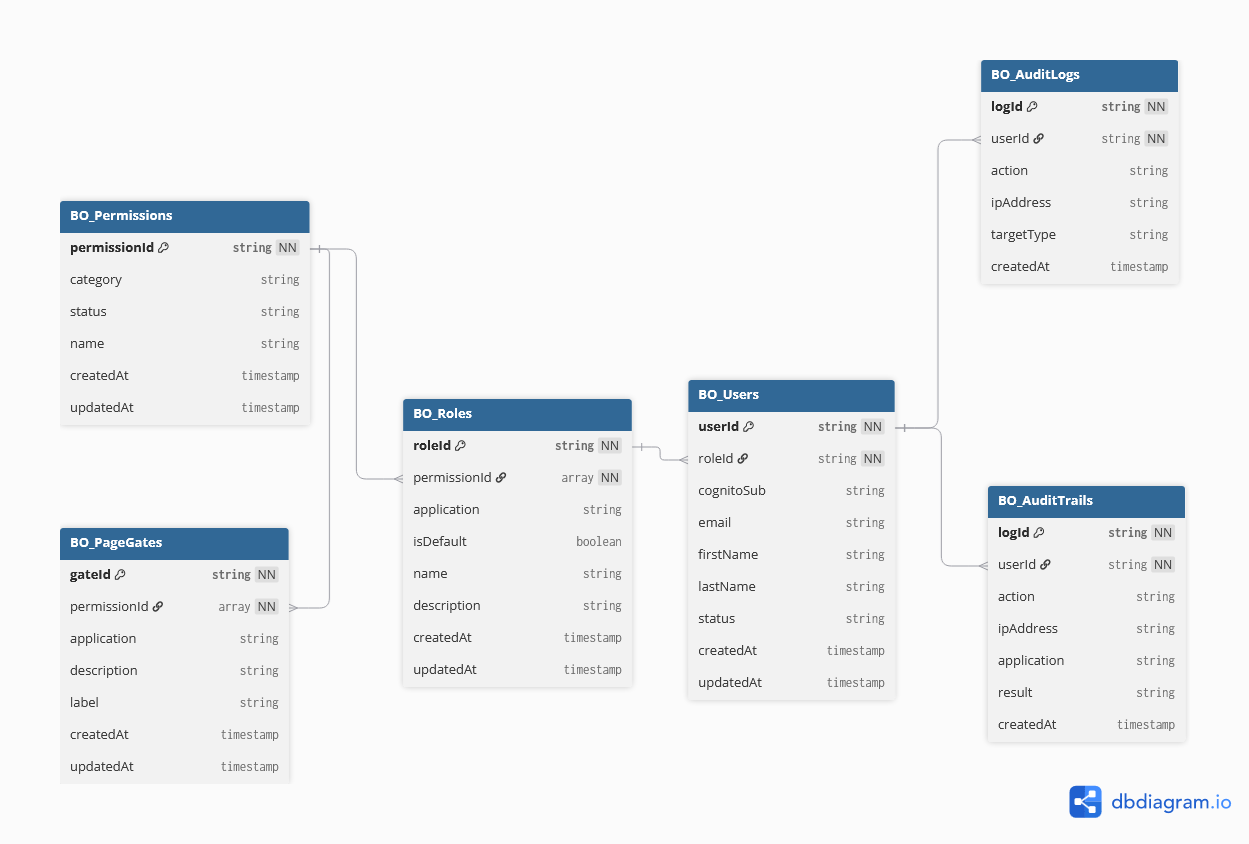
\includegraphics[width=0.95\textwidth, height=0.82\textheight, keepaspectratio]{frontmatter/assets/backoffice/ch3/uml/architecture/backoffice-data-model.png}
\caption{Modelo de dados administrativo do backoffice}
\label{fig:backoffice_data_model}
\end{figure}

Depois da Figura~\ref{fig:backoffice_data_model}, a leitura principal é a centralidade do operador interno no modelo administrativo. A tabela \texttt{BO\_Users} liga a identidade autenticada no Cognito ao perfil ou perfis de acesso configurados no backoffice. As tabelas \texttt{BO\_Roles}, \texttt{BO\_Permissions} e \texttt{BO\_PageGates} suportam a autorização: os perfis agregam permissões, e os \textit{page gates} definem que permissões permitem abrir cada área da aplicação. A auditoria fica associada ao utilizador que executou ou tentou executar a ação através de \texttt{BO\_Logs}. Esta tabela guarda tanto ações administrativas como eventos de acesso, sendo a distinção feita pelo tipo de ação e pelos filtros usados na interface. Esta relação evita registos anónimos dentro do contexto administrativo. A Tabela~\ref{tab:modelo_dados_admin} resume a responsabilidade de cada tabela.
}{}

\begin{table}[H]
\caption{Tabelas administrativas do backoffice em DynamoDB}
\label{tab:modelo_dados_admin}
\begin{center}
\small
\begin{tabular}{|l|p{9cm}|}
\hline
\textbf{Tabela} & \textbf{Responsabilidade} \\ \hline
\texttt{BO\_Users} & Guarda os operadores internos, estado da conta, identificador Cognito, e-mail e referência aos perfis atribuídos. A relação com \texttt{BO\_Roles} deve ser lida em conjunto com a regra funcional de um perfil por aplicação. \\ \hline
\texttt{BO\_Roles} & Guarda os perfis de acesso, cada um associado a uma aplicação e a um conjunto de permissões dessa mesma aplicação. \\ \hline
\texttt{BO\_Permissions} & Guarda as permissões disponíveis para autorização granular, agrupadas por categoria e usadas por perfis e \textit{page gates}. \\ \hline
\texttt{BO\_PageGates} & Guarda a configuração de acesso a páginas por aplicação, incluindo a identificação da página e as permissões aceites para a abrir. \\ \hline
\texttt{BO\_Logs} & Guarda ações administrativas, tentativas de acesso e eventos de autenticação ou navegação relevantes, sempre associados a um utilizador interno, a uma marca temporal e ao contexto necessário para consulta por filtros. \\ \hline
\end{tabular}
\end{center}
\end{table}

Depois da Tabela~\ref{tab:modelo_dados_admin}, a leitura principal é que a escalabilidade do backoffice está concentrada num modelo administrativo próprio. Ao guardar operadores, perfis, permissões, \textit{page gates} e auditoria fora dos dados transacionais da JustCauses, o sistema consegue acrescentar novas aplicações sem misturar configuração transversal com entidades específicas de cada produto. Esta tabela deve ser lida em conjunto com a Figura~\ref{fig:domain_model} e com a Figura~\ref{fig:backoffice_data_model}: o primeiro diagrama mostra o domínio global administrado pelo painel, enquanto o segundo identifica as estruturas persistidas que pertencem ao núcleo administrativo do backoffice.

\subsubsection{Modelo de permissões}
\label{sec:modelo_permissoes}

O modelo de permissões não foi tratado apenas como uma lista de perfis. Na implementação real, a autorização resulta da combinação entre o contexto do operador, a aplicação em causa e a ação concreta pedida ao sistema. A autenticação é comum, mas a autorização é resolvida depois, com base nos dados internos do backoffice.

Em termos práticos, há dois grandes contextos de utilização: o backoffice de gestão e o painel operacional da JustCauses. Ambos partilham a mesma autenticação Cognito, mas o acesso efetivo é refinado por três decisões sucessivas: acesso à aplicação, acesso à página e autorização da ação pedida à \gls{API}. Esta decomposição permite alinhar a interface, o \textit{router}, o \textit{middleware} da \gls{API} e o sistema de auditoria sob a mesma regra de negócio.

Assim, o desenho do modelo de permissões responde a quatro perguntas principais: o operador autenticado pode entrar na aplicação pedida; pode abrir a página para a qual foi encaminhado; pode executar a ação disponível na interface; e o servidor deve aceitar ou rejeitar o pedido \gls{HTTP} correspondente.

Quando o operador inicia sessão, o token do Cognito identifica a sessão, mas não chega para decidir o acesso às áreas internas. O \textit{back-end} localiza o registo do utilizador interno, verifica se a conta está ativa e resolve os perfis associados ao campo \texttt{roleIds}. O campo antigo \texttt{roleId} mantém-se apenas como compatibilidade com dados legados e representa, quando existe, o primeiro perfil do utilizador.

O modelo atual permite que um operador tenha zero ou mais perfis aplicacionais, mas impõe duas regras: só pode existir um perfil por aplicação e um perfil de backoffice é exclusivo, não podendo ser combinado com perfis aplicacionais. As permissões também têm uma aplicação associada; por isso, uma permissão da JustCauses não pode ser atribuída a um perfil de backoffice, e o servidor rejeita essa configuração mesmo que a interface tente enviá-la.

Depois de resolver os perfis, o servidor calcula o acesso efetivo: lista de perfis, permissões globais, permissões agrupadas por aplicação e aplicações acessíveis. Esta resolução centralizada evita que cada página tenha de interpretar o modelo de autorização de forma diferente.

A Tabela~\ref{tab:camadas_autorizacao} resume as camadas em que a autorização é aplicada.

\begin{table}[H]
\caption{Camadas de aplicação do modelo de autorização}
\label{tab:camadas_autorizacao}
\begin{center}
\small
\begin{tabular}{|p{3cm}|p{3.4cm}|p{7cm}|}
\hline
\textbf{Camada} & \textbf{Fonte de decisão} & \textbf{Regra aplicada} \\ \hline
Resolução do contexto & Cognito + \texttt{BO\_Users} + \texttt{BO\_Roles} + \texttt{BO\_Permissions} & O sistema valida o token, confirma o estado da conta, resolve os perfis atribuídos e calcula permissões efetivas por aplicação. \\ \hline
Guardas de rota & React Router & \texttt{ProtectedRoute} exige sessão; \texttt{BackofficeRoute} e \texttt{PanelRoute} usam a lista de aplicações acessíveis para decidir a entrada. \\ \hline
Acesso a páginas & \texttt{BO\_PageGates} & Cada página declara as permissões mínimas necessárias; quando há várias permissões, aplica-se lógica OR. \\ \hline
Ações na interface & \texttt{usePermission} & Botões e ações sensíveis só são apresentados quando a permissão necessária existe no contexto do utilizador. \\ \hline
\gls{API} & \texttt{requirePermission} & O servidor revalida permissões antes de executar a operação, devolve \texttt{401}/\texttt{403} quando necessário e regista acessos negados. \\ \hline
\end{tabular}
\end{center}
\end{table}

Depois da Tabela~\ref{tab:camadas_autorizacao}, o que se deve retirar é que a autorização é deliberadamente redundante. A interface filtra aplicações, páginas e ações para guiar o operador, mas a \gls{API} revalida os pedidos antes de alterar dados. Esta opção foi escolhida para evitar que a segurança dependesse apenas do cliente.

Existem também regras de exceção explícitas. O Super Admin recebe todas as permissões efetivas e mantém a capacidade de administração global. Os perfis de backoffice, incluindo o Backoffice Admin, têm acesso global às aplicações fora do próprio backoffice, mas só recebem permissões administrativas de backoffice quando estas estão guardadas no respetivo perfil, mantendo ainda as restrições já definidas para ações sobre utilizadores de nível equivalente ou superior. Em sentido inverso, um perfil associado apenas a \texttt{just\_causes} não pode entrar no backoffice administrativo. Um operador sem perfis atribuídos fica autenticado, mas sem acesso funcional a aplicações internas.

Esta opção evita uma matriz estática demasiado rígida. Em vez de fixar todas as relações entre perfis e páginas no código, as permissões disponíveis, os perfis e os \textit{page gates} ficam persistidos no DynamoDB, nas tabelas \texttt{BO\_Permissions}, \texttt{BO\_Roles} e \texttt{BO\_PageGates}. Como cada perfil e cada permissão têm uma aplicação associada, a integração de uma nova aplicação segue o mesmo padrão conceptual: definir permissões da aplicação, criar perfis dessa aplicação e configurar os respetivos \textit{page gates}.

%----------------------------------------------------------------------------------------

\section{Sumário}
\label{sec:sumario_cap3}

Este capítulo descreveu os requisitos, a análise do domínio, a arquitetura e o desenho do backoffice multiaplicação, tendo a JustCauses como primeira aplicação operacional integrada. A análise concentrou-se nos mecanismos que sustentam o comportamento do sistema: separação entre aplicações, resolução centralizada de permissões, \textit{page gates}, auditoria e revalidação no \textit{back-end}. Os requisitos funcionais foram organizados em treze capacidades centrais, com destaque para autenticação, autorização, operação da plataforma, verificação \gls{KYC}/\gls{KYB} e rastreabilidade. A arquitetura adotada, descrita com recurso a C4+1, separa o \textit{front-end} React do \textit{back-end} Node.js, com persistência em \gls{PostgreSQL} e DynamoDB e infraestrutura na AWS. O modelo de permissões é tratado como um mecanismo transversal que decide, em cada pedido, as aplicações, páginas e ações acessíveis ao operador. O capítulo seguinte descreve como esse desenho foi concretizado no código e na interface.

\chapter{Implementação da Solução}
\label{cap:implementação}

Neste capítulo descreve-se a implementação do backoffice multiaplicação, apresentando as soluções técnicas adotadas e evidências do trabalho desenvolvido. A JustCauses é a primeira aplicação operacional integrada e, por isso, recebe maior detalhe funcional. A estrutura do capítulo começa pelos módulos transversais ao ecossistema, como autenticação, controlo de acesso, gestão de operadores e auditoria, e depois descreve os módulos operacionais da JustCauses. No final, são apresentados os testes e a avaliação da solução, separando a descrição do que foi implementado da análise sobre como esse trabalho foi validado.

%----------------------------------------------------------------------------------------

\section{Ambiente e estrutura do projeto}
\label{sec:ambiente_infraestrutura}

O repositório está organizado em duas pastas raiz independentes: \texttt{be/} para o \textit{back-end} e \texttt{fe/} para o \textit{front-end}, cada uma com a sua configuração de dependências e de compilação. O \textit{back-end} arranca com \texttt{ts-node} em modo de desenvolvimento e compila para JavaScript em produção; o \textit{front-end} usa o servidor de desenvolvimento do Vite com \textit{Hot Module Replacement}. O controlo de versões segue uma estratégia de \textit{branching} com ramos de funcionalidade (\texttt{feature/*}) e revisão de código por \textit{pull request} antes da integração no ramo principal.

A injeção de dependências no \textit{back-end} é configurada no ficheiro \texttt{be/src/loaders/index.ts}, que regista todos os repositórios, serviços e controladores no contentor do TypeDI antes de o Express montar as rotas. Esta separação garante que as dependências são resolvidas em tempo de arranque e não em tempo de pedido, evitando instanciações desnecessárias.

A entrega para o ambiente de desenvolvimento está parcialmente automatizada com Bitbucket Pipelines, em fluxos separados para o \textit{front-end} e para o \textit{back-end}. No \textit{front-end}, cada atualização ao ramo \texttt{developer} instala as dependências, executa a \textit{build} com Vite, publica a pasta \texttt{dist/} num \textit{bucket} Amazon S3 dedicado ao ambiente de desenvolvimento e invalida a distribuição CloudFront para garantir a propagação imediata dos novos \textit{assets}. No \textit{back-end}, o pipeline constrói uma imagem Docker da aplicação, autentica-se no Amazon ECR através da AWS CLI, aplica uma etiqueta imutável baseada em \textit{timestamp} UTC e publica tanto essa versão como a etiqueta \texttt{latest}. Esta separação permitiu iterar a interface e a \gls{API} com ritmos diferentes sem introduzir acoplamento desnecessário no processo de entrega.

%----------------------------------------------------------------------------------------

\section{Autenticação e controlo de acesso}
\label{sec:autenticacao_impl}

A autenticação é gerida pelo AWS Cognito com o fluxo OAuth 2.0 / JWT padrão. No entanto, o elemento central da implementação não é apenas o \textit{login}; é a sequência de decisões que ocorre depois: identificar o operador, determinar a que aplicação pode aceder, definir que páginas pode abrir e decidir que pedidos o \textit{back-end} deve aceitar ou rejeitar. Para tornar este mecanismo mais claro, a sua implementação é descrita aqui por passos.

\subsection{Passo 1: autenticar e resolver o contexto do operador}
\label{subsec:auth_step1}

No \textit{front-end}, a sessão é gerida pelo AWS Amplify. Depois de uma autenticação bem-sucedida, o \texttt{AuthProvider} não fica apenas com os dados básicos devolvidos pelo Cognito. Faz também um pedido ao endpoint \texttt{/users/me} para obter o contexto interno do operador: identificador no backoffice, perfis atribuídos, aplicações acessíveis, permissões efetivas e permissões agrupadas por aplicação. Esta segunda leitura é necessária, porque o token Cognito identifica a sessão, mas não descreve sozinho as regras de autorização do painel.

No \textit{back-end}, esse contexto é montado no \textit{middleware} \texttt{cognitoAuth.ts}. O token Bearer é validado contra o \textit{JWKS} público do Cognito, o \texttt{token\_use} tem de ser \texttt{access}, o \texttt{client\_id} tem de coincidir com a configuração da aplicação e o \texttt{sub} do Cognito é usado para localizar o operador na base de dados interna. Só depois disso o sistema resolve os perfis guardados em \texttt{roleIds}, lê as permissões disponíveis e calcula o acesso efetivo através de uma função central. O resultado é anexado a \texttt{req.auth}, incluindo \texttt{roles}, \texttt{permissions}, \texttt{permissionsByApplication}, \texttt{appsAccessible} e \texttt{isSuperAdmin}. Se a conta não existir no backoffice ou estiver desativada, o pedido é rejeitado logo neste ponto.

O excerto da Listagem~\ref{lst:effective_access} mostra o ponto onde a autorização passa a depender também da aplicação associada a cada perfil e a cada permissão.

\begin{lstlisting}[caption={Excerto do cálculo do acesso efetivo por aplicação}, label={lst:effective_access}]
const backofficeRole =
  roles.find(role => role.application === "backoffice") ?? null;
const isSuperAdmin =
  roles.some(role => role.name === SUPER_ADMIN_ROLE_NAME);

if (isSuperAdmin) {
  allPermissions.forEach(permission =>
    addPermission(permissionsByApplicationSets, permission),
  );
} else if (backofficeRole) {
  allPermissions
    .filter(permission => permission.application !== "backoffice")
    .forEach(permission =>
      addPermission(permissionsByApplicationSets, permission),
    );

  backofficeRole.permissions.forEach(rolePermission => {
    const permission = permissionByName.get(rolePermission.name);
    if (permission?.application === "backoffice") {
      addPermission(permissionsByApplicationSets, permission);
    }
  });
} else {
  roles.forEach(role => {
    role.permissions.forEach(rolePermission => {
      const permission = permissionByName.get(rolePermission.name);
      if (permission?.application === role.application) {
        addPermission(permissionsByApplicationSets, permission);
      }
    });
  });
}

const permissionsByApplication =
  toPlainPermissions(permissionsByApplicationSets);
\end{lstlisting}

A Listagem~\ref{lst:effective_access} mostra que a autorização é calculada no servidor e devolvida já separada por aplicação. O Super Admin recebe todas as permissões; um perfil de backoffice recebe automaticamente permissões das aplicações operacionais e apenas as permissões administrativas de backoffice que estiverem associadas ao próprio perfil; um perfil aplicacional só recebe permissões da sua aplicação. Assim, uma nova aplicação pode usar o mesmo mecanismo de autenticação e autorização sem criar uma matriz fixa de acessos no cliente.

Há três exceções públicas a esta regra global, relacionadas com verificação de estado da \gls{API}, registo de falhas de autenticação e registo de tentativas de acesso. Mesmo nesses casos, a implementação tenta anexar autenticação opcional quando existe um token, sem bloquear o pedido se ele faltar ou for inválido.

\subsection{Passo 2: decidir o acesso à aplicação e à página}
\label{subsec:auth_step2}

O roteamento protegido do \textit{front-end} está dividido em quatro guardas: \texttt{ProtectedRoute}, \texttt{PublicRoute}, \texttt{BackofficeRoute} e \texttt{PanelRoute}. A diferença relevante está nas duas últimas: uma controla o acesso ao backoffice administrativo e a outra controla o acesso ao painel operacional pedido, neste caso a JustCauses. Quando a aplicação é recusada, a interface apresenta um ecrã de acesso negado e envia, em segundo plano, um registo de tentativa falhada.

Depois de entrar na aplicação certa, o sistema ainda tem de decidir a que página encaminhar o operador. Essa decisão é feita duas vezes. Primeiro, no \textit{router}, através das listas \texttt{PANEL\_PAGES} e \texttt{ADMIN\_PAGES}, que definem a permissão base de cada rota e calculam o primeiro destino acessível. Depois, já dentro dos \textit{layouts}, através dos \textit{page gates} carregados da \gls{API}. No painel JustCauses, o \textit{layout} aplica lógica OR às permissões configuradas. No backoffice administrativo, as ações mais sensíveis continuam dependentes das permissões administrativas e das restrições de nível dos operadores.

Esta combinação separa duas decisões distintas. As guardas de rota determinam se o operador pode entrar numa aplicação. Os \textit{page gates} determinam se uma página concreta deve aparecer na navegação e ser renderizada.

\subsection{Passo 3: limitar ações dentro da interface}
\label{subsec:auth_step3}

Mesmo quando a página já está aberta, nem todas as ações são mostradas a todos os operadores. Para isso existe o \textit{hook} \texttt{usePermission}, usado em páginas e componentes para esconder botões, ações rápidas e controlos de edição. A regra usa as permissões efetivas devolvidas pelo servidor: o Super Admin passa sempre; nos restantes casos, a ação só aparece se a permissão necessária estiver presente no contexto do utilizador.

No painel, esconder uma ação é uma decisão de experiência de utilização, não uma garantia de segurança. Esta filtragem reduz elementos indisponíveis na interface e torna mais clara a área de responsabilidade de cada operador. A validação de segurança continua a ser feita no servidor.

\subsection{Passo 4: revalidar cada pedido no servidor}
\label{subsec:auth_step4}

Todas as rotas da \gls{API} são montadas sob autenticação Cognito, definida no carregador do Express. Sobre essa autenticação base, os endpoints sensíveis usam o \textit{middleware} de autorização. O padrão repete-se de forma consistente ao longo do código: a listagem de campanhas exige \texttt{view\_campaigns}; a criação ou edição de categorias recorre a \texttt{change\_settings}; e a consulta de logs aceita \texttt{view\_audit\_logs} ou \texttt{view\_admin\_logs}. Nas restantes rotas operacionais, a lógica mantém-se: o pedido só avança quando traz uma das permissões aceites para essa operação.

O comportamento do \textit{middleware} é deliberadamente conservador. Se não existir contexto de autenticação, o pedido recebe \texttt{401}. Se o utilizador estiver autenticado mas não tiver nenhuma das permissões exigidas, recebe \texttt{403}. O Super Admin contorna sempre esta validação. Os restantes operadores, incluindo perfis de backoffice, passam apenas quando a permissão existe no conjunto de permissões efetivas calculado previamente pelo servidor. Assim, a regra especial de backoffice é tratada na resolução central de acesso, não espalhada por cada rota.

Quando um pedido é recusado por falta de permissões, o servidor infere a aplicação a partir da rota, regista o evento \texttt{APP\_ACCESS\_FAILED} e aplica uma janela curta de deduplicação para limitar eventos repetidos do mesmo utilizador sobre o mesmo recurso. Esta regra reduz redundância nos registos de auditoria, sobretudo em cenários de atualização repetida de páginas sem acesso.

O excerto da Listagem~\ref{lst:require_permission} mostra o núcleo desta segunda validação no servidor.

\begin{lstlisting}[caption={Validação de permissões no middleware \texttt{requirePermission}}, label={lst:require_permission}]
export function requirePermission(...required) {
  return (req, res, next) => {
    const auth = req.auth;
    if (!auth) {
      res.status(401).json({ message: "Unauthorized" });
      return;
    }

    if (auth.isSuperAdmin) {
      next();
      return;
    }

    const hasPermission = required.some((p) =>
      auth.permissions.includes(p),
    );

    if (!hasPermission) {
      res.status(403).json({
        message: "Forbidden: insufficient permissions",
      });
      return;
    }

    next();
  };
}
\end{lstlisting}

%----------------------------------------------------------------------------------------

\section{Módulos transversais ao ecossistema}
\label{sec:modulos_transversais}

\subsection{Seletor de aplicações}
\label{subsec:impl_app_selector}

Após a autenticação, o operador é encaminhado para o seletor de aplicações. A página apresenta exclusivamente as aplicações para as quais o operador tem um perfil atribuído, pelo que dois operadores com acessos diferentes veem listas distintas. O botão de gestão do backoffice administrativo só é visível para operadores com um perfil de backoffice, sendo ocultado para todos os restantes. Esta filtragem é uma consequência direta do modelo de autorização por aplicação: a interface não esconde arbitrariamente opções, limita-se a refletir o contexto de acesso calculado pelo servidor após a autenticação.

\subsection{Gestão de operadores, perfis e permissões}
\label{subsec:impl_roles_permissions}

A página de gestão de utilizadores internos permite criar contas de backoffice, ativar ou desativar operadores, transferir o papel de Super Admin e gerir o acesso atribuído a cada utilizador. Com a evolução do modelo de autorização, a atribuição deixou de depender de um único campo \texttt{roleId} e passou a trabalhar sobre \texttt{roleIds}. Na interface, o administrador escolhe no máximo um perfil por aplicação; se selecionar um perfil de backoffice, as restantes aplicações ficam bloqueadas, porque os perfis de backoffice são globais e exclusivos.

A página de perfis e permissões aplica a mesma separação. Cada perfil pertence a uma aplicação, e a interface apenas apresenta permissões dessa aplicação. Esta filtragem reduz o risco de erro operacional, mas não é a garantia principal: o \textit{back-end} volta a validar a associação antes de gravar alterações e rejeita permissões cuja aplicação não corresponda à aplicação do perfil.

As validações centrais desta regra aparecem na Listagem~\ref{lst:role_permission_validation}. O excerto mostra duas barreiras complementares: a atribuição de perfis a operadores e a associação de permissões a perfis.

\begin{lstlisting}[caption={Validações de perfis e permissões por aplicação}, label={lst:role_permission_validation}]
const applications = new Set<string>();
for (const role of roles) {
  if (applications.has(role.application)) {
    throw this.buildError(
      "ROLE_APPLICATION_DUPLICATE",
      "A user can only have one role per application.",
    );
  }
  applications.add(role.application);
}

if (
  roles.some(role => role.application === "backoffice") &&
  roles.length > 1
) {
  throw this.buildError(
    "BACKOFFICE_ROLE_EXCLUSIVE",
    "Backoffice roles are global and cannot be combined " +
      "with application roles.",
  );
}

private assertPermissionMatchesRoleApplication(
  application: RoleApplication,
  permission: Permission,
): void {
  if (permission.application !== application) {
    throw this.buildError(
      "PERMISSION_APPLICATION_MISMATCH",
      `Permission "${permission.name}" belongs to ` +
        `"${permission.application}" and cannot be assigned to ` +
        `a "${application}" role.`,
    );
  }
}
\end{lstlisting}

A Listagem~\ref{lst:role_permission_validation} mostra que a coerência do modelo não depende apenas da interface. O servidor impede dois casos que comprometeriam a evolução futura: atribuir dois perfis da mesma aplicação ao mesmo operador e misturar um perfil global de backoffice com perfis aplicacionais. A mesma lógica impede que uma permissão da JustCauses seja guardada num perfil de backoffice, ou o inverso.

Esta implementação é uma das principais evidências de escalabilidade do backoffice. Para acrescentar uma nova aplicação, o modelo não exige criar uma lógica de autorização paralela; exige definir as permissões da aplicação, criar perfis associados e configurar as páginas correspondentes. O mecanismo de resolução de acesso continua o mesmo.

\subsection{Configuração administrativa do acesso}
\label{subsec:impl_access_admin}

A área \texttt{/admin} concentra as ferramentas administrativas que mantêm o modelo de autorização operacional. Nela existem páginas para gerir contas internas, ajustar perfis e configurar os \textit{page gates} das duas aplicações. Neste relatório, estas páginas não são tratadas como módulos funcionais isolados; são apresentadas como a consola onde o mecanismo de autorização é mantido e configurado.

A \texttt{PageGatesPage} carrega as configurações por aplicação e permite associar a cada página um conjunto de permissões. A regra usada tanto na interface como no \textit{back-end} é explícita: quando uma página lista várias permissões, o operador precisa de ter pelo menos uma delas. Isto permite adaptar o acesso sem alterar o código das rotas e sem novo \textit{deploy}, porque a configuração fica persistida em DynamoDB.

Também aqui foi mantido o padrão \textit{draft}. O operador pode preparar alterações, compará-las com o estado atual e só depois decidir guardar ou descartar. Num módulo sensível como o de autorização, esta opção reduz o risco de mudanças acidentais aplicadas à primeira interação.

\subsection{Sistema de auditoria}
\label{subsec:impl_audit}

Todas as operações de escrita realizadas por operadores sobre entidades críticas geram um registo de auditoria no AWS DynamoDB. Cada registo contém o identificador do ator, o tipo e identificador da entidade afetada, a ação executada, a marca temporal em ISO 8601 e metadados adicionais específicos da ação (razão, estado anterior, estado novo). Os registos são imutáveis: não existem operações de atualização ou eliminação no \texttt{AuditLogRepo}.

A página \texttt{LogsPage} permite consultar o histórico de auditoria com filtros por data, por operador e por tipo de ação. Para além das ações de negócio, o sistema passou também a registar tentativas falhadas de acesso à aplicação e recusas por permissões insuficientes. No \textit{front-end}, esse envio é feito de forma não bloqueante; no \textit{back-end}, a recusa é registada no próprio \textit{middleware} de autorização. A chave de partição no DynamoDB é o identificador da entidade, com a marca temporal como chave de ordenação, o que garante uma consulta eficiente por entidade e por intervalo de tempo.

A dimensão de responsabilização foi reforçada com o botão \textbf{Activity} na página de utilizadores internos. Este botão abre uma vista agregada da atividade de um operador, combinando eventos de \textit{audit logs} e \textit{audit trail}. A consulta permite filtrar por origem, ação ou evento, resultado, aplicação e intervalo temporal. Quando um registo é selecionado, a interface mostra detalhes como data, alvo, endereço IP e metadados associados. Esta vista apoia a análise operacional de questões como acessos tentados por um operador, alterações realizadas e aplicação afetada.

%----------------------------------------------------------------------------------------

\section{Módulos operacionais da JustCauses}
\label{sec:modulos_ojc}

Os módulos descritos nesta secção evidenciam a integração com os dados transacionais da plataforma e a consistência da arquitetura adotada, concentrando-se nos fluxos desenvolvidos no âmbito deste estágio.

\subsection{Dashboard e métricas}
\label{subsec:impl_dashboard}

A \texttt{AdminOverviewPage}, disponível em \texttt{/ojc} após a entrada no painel da JustCauses, é a visão operacional da plataforma. Apresenta sete métricas de resumo calculadas pelo endpoint \texttt{GET /api/ojc/overview/stats}: número total de utilizadores, campanhas ativas, volume total angariado, pedidos de aprovação pendentes, denúncias abertas, total de campanhas e doações concluídas.

O \textit{back-end} calcula estas métricas através de \textit{queries} de agregação SQL sobre a base de dados da JustCauses. Os resultados são devolvidos num único pedido e apresentados em cartões de resumo no topo da página.

\subsection{Gestão de campanhas}
\label{subsec:impl_campaigns}

O módulo de gestão de campanhas é composto por duas vistas complementares. A página \texttt{CampaignsPage}, acessível em \texttt{/ojc/campaigns}, apresenta a listagem operacional das campanhas e permite filtrar por estados como \texttt{PENDING}, \texttt{ACTIVE}, \texttt{INACTIVE}, \texttt{FINISHED}, \texttt{REJECTED} e \texttt{REVIEWING}. A revisão detalhada fica concentrada no módulo \texttt{CampaignRevisionsPage}, onde cada submissão é tratada como uma \textit{thread} de revisão.

Esta separação evita misturar duas tarefas diferentes. A listagem serve para localizar campanhas e perceber o seu estado. A \textit{thread} de revisão serve para decidir. Nessa vista, o operador consulta o resumo da campanha, o tipo de revisão, o estado atual, o número da submissão mais recente, o histórico de submissões e o histórico de decisões anteriores. Quando existe uma versão anterior, a interface apresenta uma comparação campo a campo entre o estado anterior e a submissão atual. Quando se trata da primeira submissão de uma campanha, a mesma estrutura é usada como vista dos dados submetidos.

O fluxo suporta três decisões principais: aprovar, pedir alterações ou rejeitar. Nos pedidos de alteração e rejeições, a mensagem do operador é obrigatória, porque essa informação passa a fazer parte do histórico da \textit{thread} e é usada para orientar o criador. Esta mensagem é persistida, apresentada no painel e enviada por e-mail quando aplicável. Assim, a revisão não fica reduzida a uma mudança de estado; fica associada a um motivo, a um operador e a uma data.

Cada ação de revisão gera automaticamente um registo de auditoria no DynamoDB e uma notificação por e-mail ao criador via \gls{SES}. O conteúdo do e-mail depende da decisão tomada: aprovação, rejeição ou pedido de alterações. Quando existe uma mensagem do operador, esta é incluída no corpo da comunicação para que o criador compreenda a decisão e saiba que passos deve executar de seguida.

\subsection{Gestão de categorias}
\label{subsec:impl_categories}

O módulo de categorias, acessível na página \texttt{CategoriesPage} em \texttt{/ojc/categories}, implementa a gestão completa das categorias temáticas das campanhas. Cada categoria é definida por um nome único, um \textit{slug} de URL, um ícone (\texttt{iconName}), uma descrição e um estado de ativação (\texttt{isActive}).

O \textit{back-end} expõe quatro endpoints para este módulo: \texttt{GET} \path{/api/ojc/categories} para listagem; \texttt{POST} \path{/api/ojc/categories} para criação; \texttt{PATCH} \path{/api/ojc/categories/:id} para edição, incluindo desativação através de \texttt{isActive: false}; e \texttt{DELETE} \path{/api/ojc/categories/:id} para remoção. A criação e a edição validam a unicidade do nome e do \textit{slug}, devolvendo \texttt{409 Conflict} em caso de duplicado. Todas as operações de escrita são registadas no sistema de auditoria, com a ação \texttt{CATEGORY\_DELETED} para eliminações.

\subsection{Verificação KYC e KYB}
\label{subsec:impl_kyc_kyb}

A JustCauses distingue criadores individuais de organizações. Esta distinção não altera o princípio geral do backoffice, mas altera a validação operacional necessária antes de determinados fluxos sensíveis. Utilizadores individuais são acompanhados através de \gls{KYC}; organizações são acompanhadas através de \gls{KYB}. Em ambos os casos, o objetivo do painel é dar ao operador uma vista verificável dos dados submetidos, permitir uma decisão controlada e deixar rasto auditável da ação.

No fluxo \gls{KYC}, a página \texttt{KycQueuePage}, acessível em \texttt{/ojc/kyc}, carrega a fila de verificações através de \texttt{GET} \path{/api/ojc/kyc}. O endpoint é protegido por \texttt{requirePermission("view\_kyc")} e devolve submissões filtráveis por estado, pesquisa, país, tipo de documento, comparação de dados e atraso da submissão. O repositório combina informação das tabelas partilhadas de verificação com perfis da JustCauses, permitindo comparar os dados declarados no perfil com os dados devolvidos pelo fornecedor externo. A interface destaca diferenças de nome e país, falta de dados do fornecedor e submissões pendentes há mais de sete dias.

Quando são detetadas inconsistências, o operador pode preparar um aviso por e-mail ao utilizador. O \textit{back-end} valida a submissão, envia a mensagem através do serviço de e-mail e regista a ação \texttt{KYC\_MISMATCH\_WARNING\_SENT}. Quando uma submissão pendente fica desatualizada, o sistema permite repor o processo, removendo a submissão pendente, criando uma notificação interna e enviando um e-mail de reinício de verificação. A ativação ou desativação de conta aparece apenas como consequência operacional possível dentro deste contexto de revisão, não como foco principal do módulo.

No fluxo \gls{KYB}, a página de organizações apresenta perfis coletivos da JustCauses e permite ao operador abrir a informação de verificação de uma organização. A listagem é acedida através de \texttt{GET} \path{/api/ojc/organizations}, protegida por \texttt{view\_organizations} ou \texttt{view\_kyb}; já as decisões \gls{KYB} exigem \texttt{view\_kyb}. A submissão contém documentos como registo da entidade, documento do representante e fotografia de confirmação, para que o operador possa avaliar a oficialidade da organização e a representação associada.

A aprovação e a rejeição são executadas através de endpoints próprios para decisão \gls{KYB}. A rejeição exige uma nota administrativa, enquanto a aprovação pode incluir uma nota opcional. O serviço atualiza a submissão \gls{KYB}, ajusta o estado de verificação do perfil da organização, cria uma notificação interna, envia e-mail de decisão quando existe endereço associado e regista a auditoria com as ações \texttt{KYB\_APPROVED} ou \texttt{KYB\_REJECTED}. Assim, a organização surge no relatório como entidade operacional da JustCauses e o contributo descrito centra-se na sua verificação, não na gestão geral de organizações.

\subsection{Comunicação por e-mail e notificações}
\label{subsec:impl_email_notifications}

As notificações por e-mail foram implementadas como consequência direta das ações de revisão de campanhas. O operador não envia manualmente estes e-mails; a decisão no painel desencadeia uma chamada no \textit{back-end}, que valida a operação, persiste a alteração, regista a auditoria e só depois solicita o envio da mensagem.

Os e-mails transacionais são enviados através do Amazon SES. O \textit{back-end} concentra esta responsabilidade num serviço de e-mail que constrói mensagens HTML com dados do domínio, como o título da campanha, a decisão tomada e a mensagem deixada pelo operador. Esta centralização evita duplicar a configuração do fornecedor e mantém os modelos de mensagem próximos das regras de negócio que os originam.

A Tabela~\ref{tab:emails_transacionais} identifica os principais e-mails automáticos associados a ações administrativas relevantes. A revisão de campanhas é o exemplo demonstrado visualmente neste relatório, mas o mesmo serviço centraliza também mensagens relacionadas com estados de conta e medidas aplicadas a utilizadores.

\begin{table}[H]
\caption{E-mails transacionais acionados por operações administrativas}
\label{tab:emails_transacionais}
\begin{center}
\footnotesize
\begin{tabular}{|p{3.5cm}|p{3.4cm}|p{6.2cm}|}
\hline
\textbf{Fluxo} & \textbf{Destinatário} & \textbf{Informação comunicada} \\ \hline
Revisão de campanha & Criador da campanha & Aprovação, rejeição ou pedido de alterações, incluindo a mensagem de revisão quando o operador a fornece. \\ \hline
Revisão de alterações a campanha publicada & Criador da campanha & Resultado da revisão da alteração submetida, distinguindo aprovação, rejeição e pedido de correção. \\ \hline
Verificação KYC & Utilizador individual & Aviso de inconsistência entre dados de perfil e dados de verificação, ou reinício de uma submissão pendente há demasiado tempo. \\ \hline
Verificação KYB & Organização & Resultado da avaliação da submissão documental, distinguindo aprovação e rejeição, com a nota administrativa quando aplicável. \\ \hline
Estado da conta & Utilizador ou organização afetada & Ativação, desativação ou alteração de estado comunicada por e-mail quando a operação administrativa exige aviso externo. \\ \hline
Medidas sobre utilizadores & Utilizador afetado & Registo ou remoção de \textit{strikes}, avisos e outras decisões operacionais que devem ficar explícitas para o utilizador. \\ \hline
\end{tabular}
\end{center}
\end{table}

Quando o e-mail complementa uma notificação interna da JustCauses, os dois mecanismos são tratados de forma independente. A notificação interna é persistida na base de dados da aplicação, enquanto o e-mail funciona como canal externo de aviso. Em caso de falha no envio, o erro fica registado nos logs do servidor, mas a operação administrativa não é revertida, porque a decisão já foi validada e persistida.

\subsection{\textit{Analytics}}
\label{subsec:impl_analytics}

O módulo de \textit{analytics}, acessível na página \texttt{AnalyticsPage} em \texttt{/ojc/analytics}, apresenta uma visão temporal e categórica do desempenho da plataforma. O \textit{back-end} expõe o endpoint \texttt{GET /api/ojc/analytics} com suporte a filtros de período (\texttt{1d}, \texttt{1w}, \texttt{2w}, \texttt{1m}, \texttt{3m}, \texttt{6m}, \texttt{1y}, \texttt{all}).

A página inclui gráficos de evolução temporal de receita, novos utilizadores e campanhas criadas; uma tabela de campanhas com mais doações angariadas, ordenada por valor total decrescente (\texttt{ORDER BY COALESCE(SUM(d."amount"), 0) DESC}); e distribuições de doações por estado e por categoria. A \textit{query} de agregação das campanhas utiliza \texttt{COALESCE} para garantir que campanhas sem doações surgem corretamente com valor zero em vez de serem excluídas.

%----------------------------------------------------------------------------------------

\section{Perspetivas de utilização e evidências}
\label{sec:evidencias_utilizador}

Para além da descrição técnica, a implementação deve ser lida a partir das perspetivas dos operadores que usam o painel. As evidências visuais desta secção mostram como o desenho descrito no Capítulo~\ref{cap:analise_desenho} foi concretizado na interface: separação de permissões, configuração de acesso, auditoria e operação da JustCauses. A Tabela~\ref{tab:evidencias_prints} identifica a perspetiva de cada evidência e o ponto que deve ser retirado pelo leitor.

Os diagramas de sequência que detalham estes fluxos foram reunidos no Apêndice~\ref{app:sd_detalhados}. Assim, esta secção mantém o foco nas evidências visuais e na interpretação do que cada ecrã demonstra.

Nas evidências relativas a \gls{KYC} e \gls{KYB}, importa distinguir a origem dos dados apresentados. A integração de \gls{KYC} com o fornecedor externo de verificação não estava disponível no ambiente de desenvolvimento por decisão da equipa responsável pela aplicação JustCauses, ficando ativa apenas em produção. Por esse motivo, as capturas de \gls{KYC} foram obtidas com dados reais anonimizados e parcialmente ocultados. Já as capturas de \gls{KYB} foram obtidas em ambiente de desenvolvimento, com dados de demonstração sem correspondência a organizações reais.

As Figuras~\ref{fig:impl_app_selector} a~\ref{fig:impl_kyb_verification_modal} apresentam as evidências visuais selecionadas para demonstrar a concretização dos principais fluxos transversais e operacionais.

\begin{table}[H]
\caption{Evidências visuais usadas no Capítulo 4}
\label{tab:evidencias_prints}
\begin{center}
\begingroup
\scriptsize
\setlength{\tabcolsep}{4pt}
\begin{tabular}{|p{2.9cm}|p{3.8cm}|p{5.9cm}|}
\hline
\textbf{Perspetiva} & \textbf{Evidência visual} & \textbf{O que deve demonstrar} \\ \hline
Entrada no ecossistema & Seletor de aplicações & O operador vê apenas as aplicações para as quais tem um perfil atribuído; o acesso ao backoffice administrativo só aparece para operadores com perfil de backoffice. \\ \hline
Gestão de operadores & Atribuição de perfis & A atribuição manual permite um perfil por aplicação e separa perfis globais de backoffice de perfis da JustCauses. \\ \hline
Perfis e permissões & Permissões por aplicação & A edição de um perfil apresenta apenas permissões da aplicação selecionada. \\ \hline
Configuração de páginas & Configuração de \textit{page gates} & O acesso a páginas é configurável por aplicação e usa permissões como regra de entrada. \\ \hline
Auditoria individual & Atividade de operador & A atividade de um operador agrega ações administrativas, eventos de acesso, resultado e aplicação. \\ \hline
Revisão de campanhas & \textit{Thread} de revisão & O operador compara submissões, consulta histórico, decide a revisão e deixa registo da operação. \\ \hline
Permissões de ação & Modal de campanha com e sem ações & A mesma campanha pode ser consultada por operadores diferentes, mas as ações sensíveis só aparecem quando o perfil tem permissão. \\ \hline
Comunicação externa & E-mail transacional & A decisão administrativa é comunicada ao criador com a mensagem registada pelo operador. \\ \hline
Gestão de categorias & Administração de categorias & O módulo gere categorias usadas na criação de campanhas e protege categorias já associadas a causas existentes. \\ \hline
Verificação KYC & Fila e modal de comparação & O operador consulta verificações individuais, identifica diferenças entre perfil e fornecedor externo e executa ações auditadas. \\ \hline
Verificação KYB & Organizações e submissão documental & O operador consulta organizações, abre a submissão documental e decide a verificação com notificação e auditoria. \\ \hline
\end{tabular}
\endgroup
\end{center}
\end{table}

\IfFileExists{frontmatter/assets/backoffice/ch4/app-selector.png}{
\begin{figure}[H]
\centering
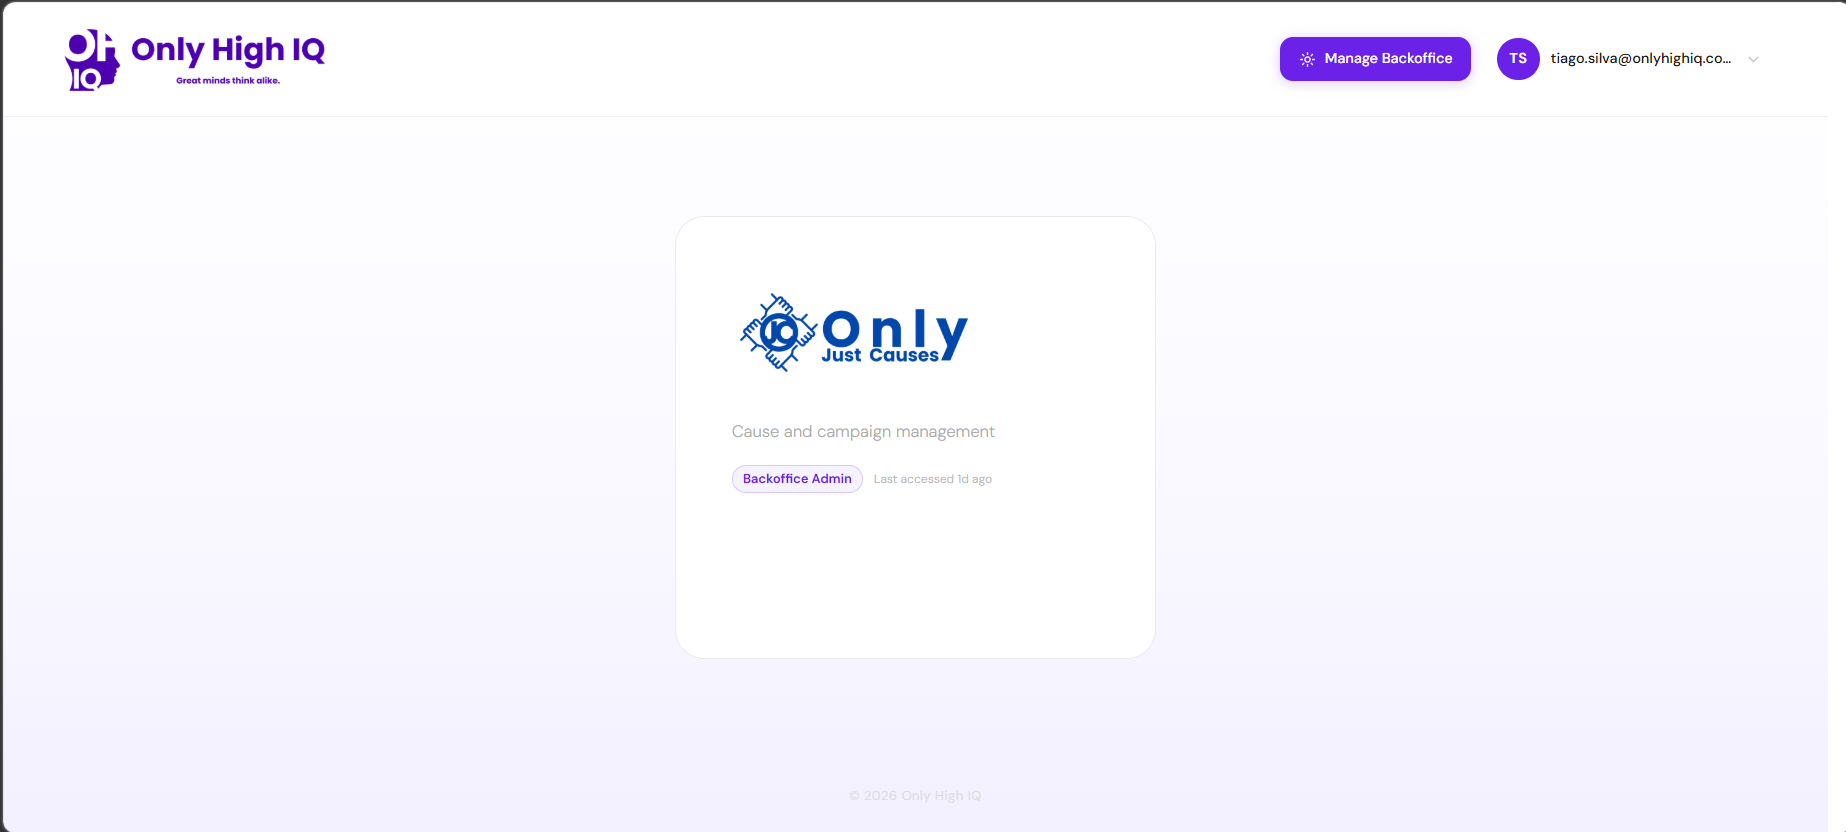
\includegraphics[width=0.95\textwidth, keepaspectratio]{frontmatter/assets/backoffice/ch4/app-selector.png}
\caption{Seletor de aplicações disponível após autenticação}
\label{fig:impl_app_selector}
\end{figure}

Depois da Figura~\ref{fig:impl_app_selector}, a leitura pretendida é que a lista de aplicações não é fixa nem genérica: resulta diretamente do perfil atribuído ao operador. No exemplo, o acesso ao backoffice administrativo aparece precisamente porque o operador tem um perfil de backoffice; para um operador sem esse perfil, o botão não seria apresentado.
}{}

\IfFileExists{frontmatter/assets/backoffice/ch4/role-assignment.png}{
\begin{figure}[H]
\centering
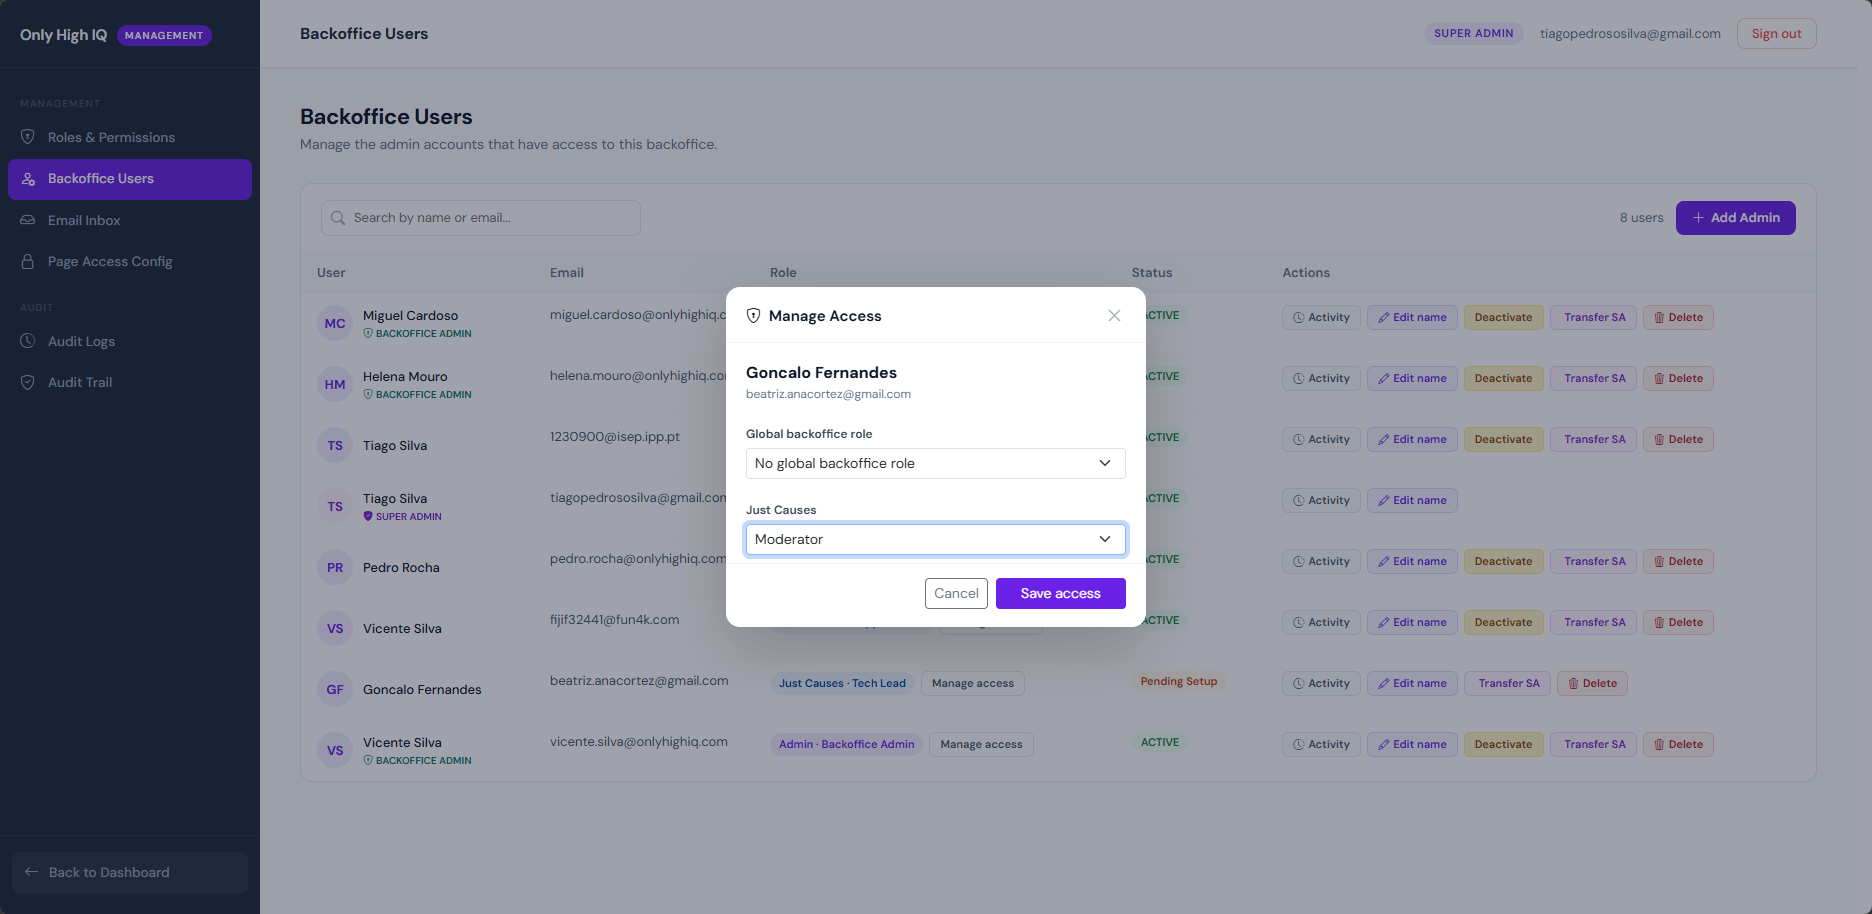
\includegraphics[width=0.95\textwidth, keepaspectratio]{frontmatter/assets/backoffice/ch4/role-assignment.png}
\caption{Atribuição de perfis a um operador interno}
\label{fig:impl_role_assignment}
\end{figure}

Depois da Figura~\ref{fig:impl_role_assignment}, a evidência a reter é que a atribuição de acesso é feita por aplicação. A janela distingue o perfil global de backoffice dos perfis da JustCauses e obriga o administrador a escolher explicitamente o acesso pretendido. Esta opção torna visível a regra usada no servidor: perfis administrativos são globais, enquanto perfis de aplicações operacionais são atribuídos no contexto da respetiva aplicação.
}{}

\IfFileExists{frontmatter/assets/backoffice/ch4/permissions-by-application.png}{
\begin{figure}[H]
\centering
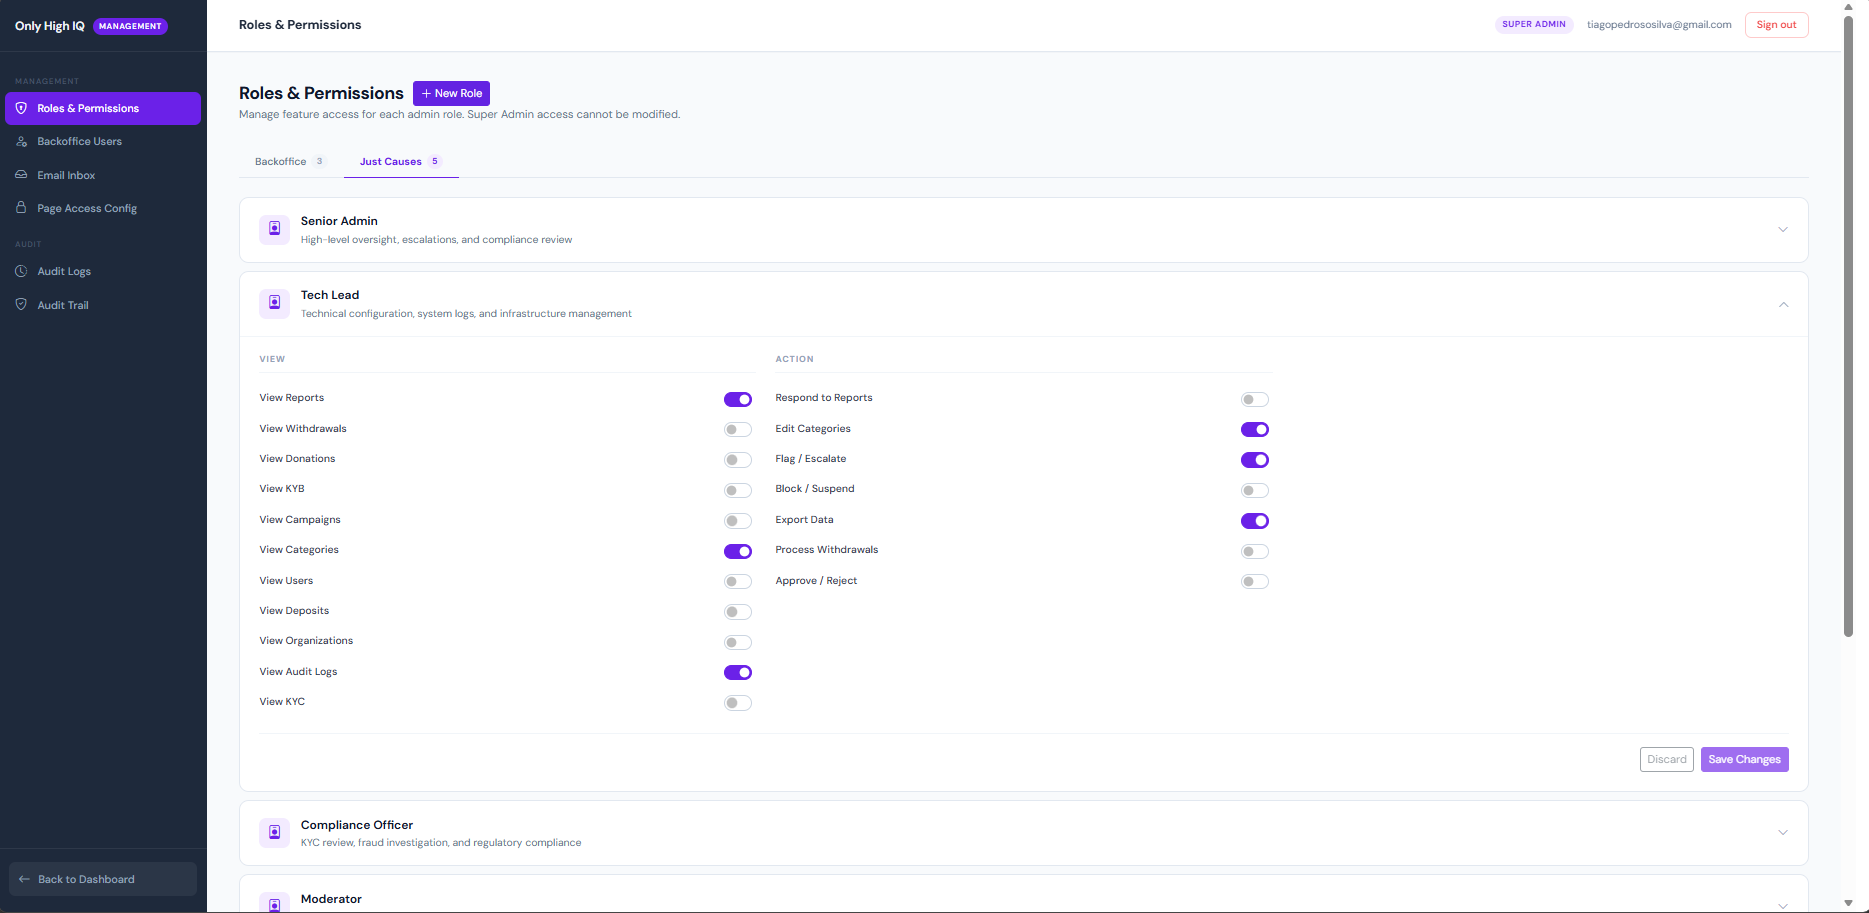
\includegraphics[width=0.95\textwidth, keepaspectratio]{frontmatter/assets/backoffice/ch4/permissions-by-application.png}
\caption{Permissões filtradas pela aplicação do perfil}
\label{fig:impl_permissions_by_application}
\end{figure}

Depois da Figura~\ref{fig:impl_permissions_by_application}, a evidência pretendida é a separação entre aplicações. O perfil aberto pertence à JustCauses e, por isso, a interface apresenta permissões ligadas a essa aplicação. A filtragem reduz erro operacional, mas não substitui a validação do servidor, que continua a rejeitar permissões cuja aplicação não corresponda à aplicação do perfil.
}{}

\IfFileExists{frontmatter/assets/backoffice/ch4/page-gates.png}{
\begin{figure}[H]
\centering
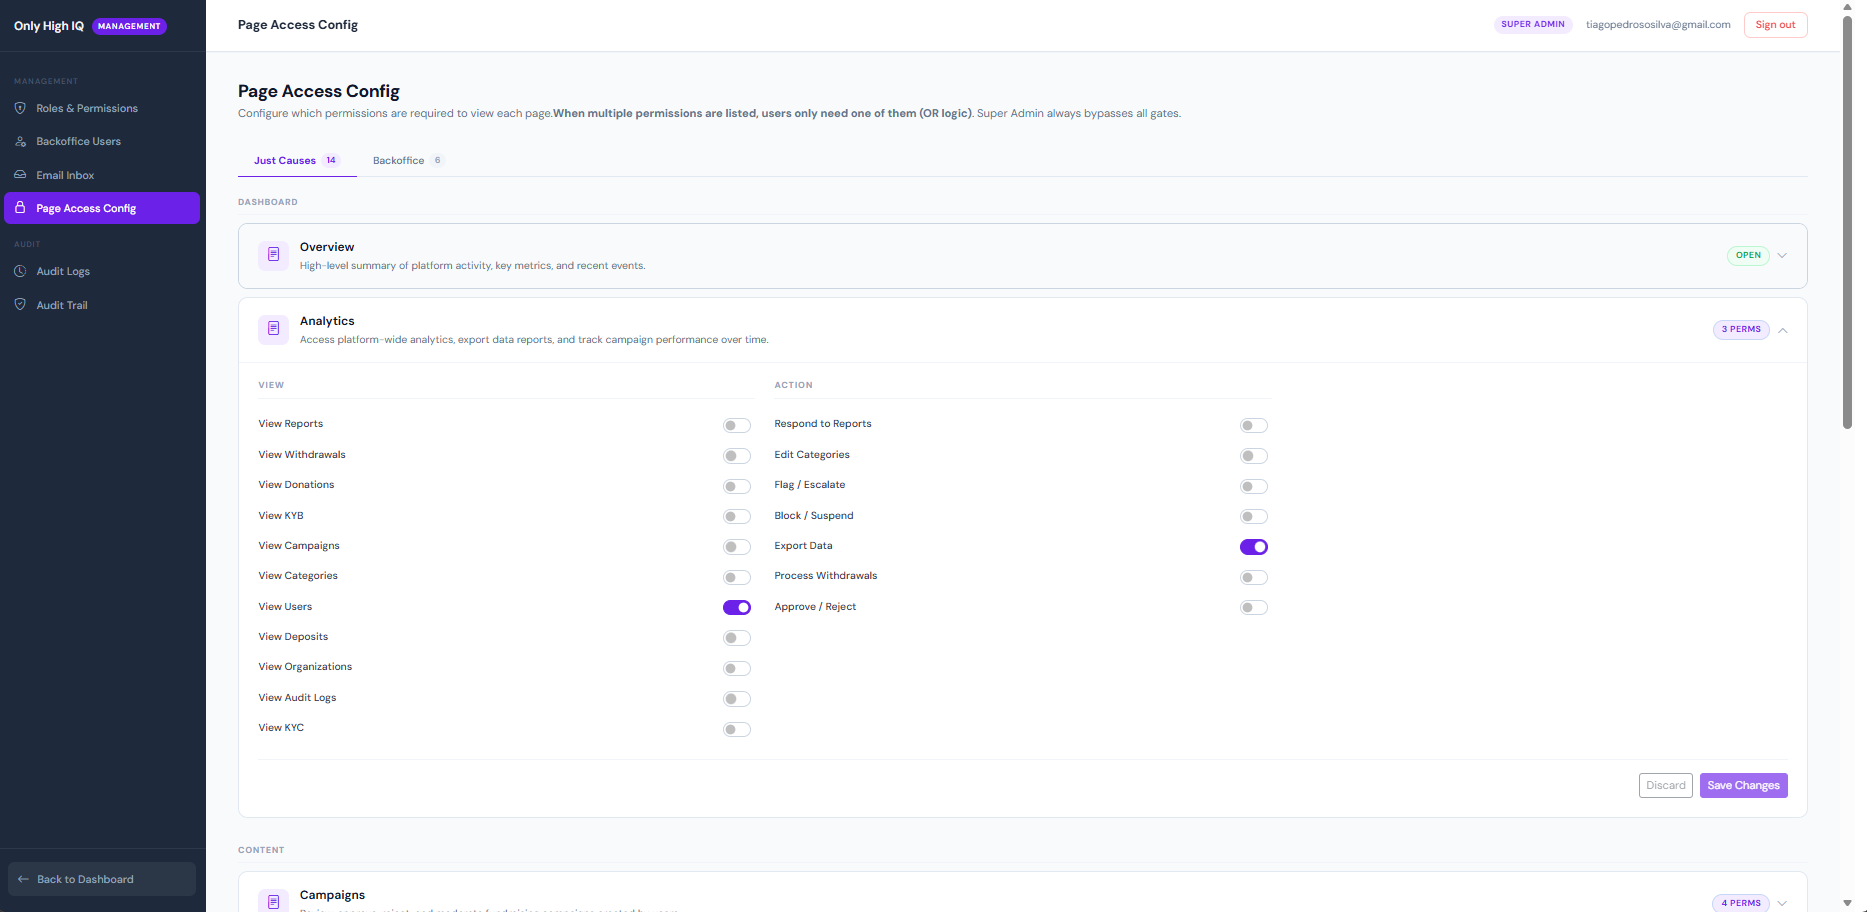
\includegraphics[width=0.95\textwidth, keepaspectratio]{frontmatter/assets/backoffice/ch4/page-gates.png}
\caption{Configuração administrativa dos \textit{page gates}}
\label{fig:impl_page_gates}
\end{figure}

Depois da Figura~\ref{fig:impl_page_gates}, importa evidenciar que o acesso a páginas não está fixo apenas no código. Cada página pode ter permissões associadas e a configuração é organizada por aplicação. No exemplo, a página de \textit{analytics} da JustCauses exige permissões específicas, enquanto páginas abertas aparecem explicitamente como \textit{open}. Esta distinção ajuda o administrador a perceber que páginas dependem de autorização e que páginas ficam disponíveis sem configuração adicional.
}{}

\IfFileExists{frontmatter/assets/backoffice/ch4/user-activity.png}{
\begin{figure}[H]
\centering
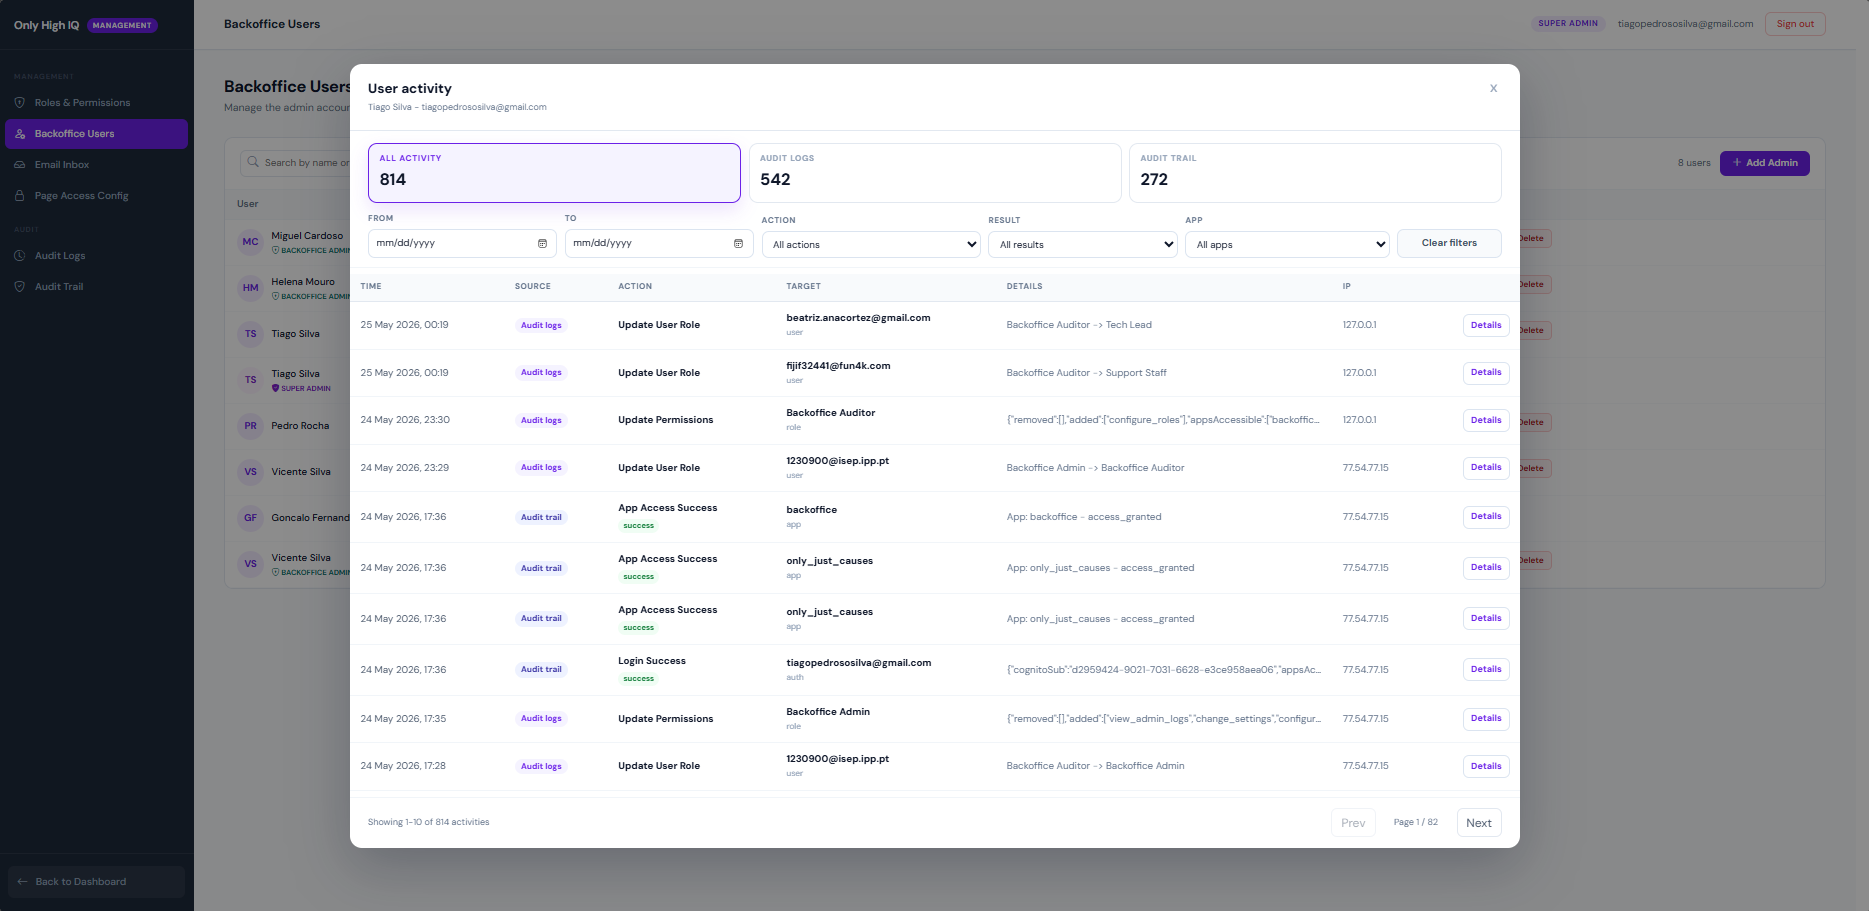
\includegraphics[width=0.95\textwidth, keepaspectratio]{frontmatter/assets/backoffice/ch4/user-activity.png}
\caption{Vista de atividade individual de um operador}
\label{fig:impl_user_activity}
\end{figure}

Depois da Figura~\ref{fig:impl_user_activity}, o objetivo é mostrar a dimensão de responsabilização. A vista agrega eventos de \textit{audit logs} e \textit{audit trail}, permite filtrar por ação, resultado e aplicação, e apresenta eventos como alterações de perfil, atualizações de permissões, acessos concedidos e início de sessão. Esta consulta apoia a análise do comportamento de um operador sem exigir navegação separada por vários registos.
}{}

\IfFileExists{frontmatter/assets/backoffice/ch4/ojc-campaign-review1.png}{
\begin{figure}[H]
\centering
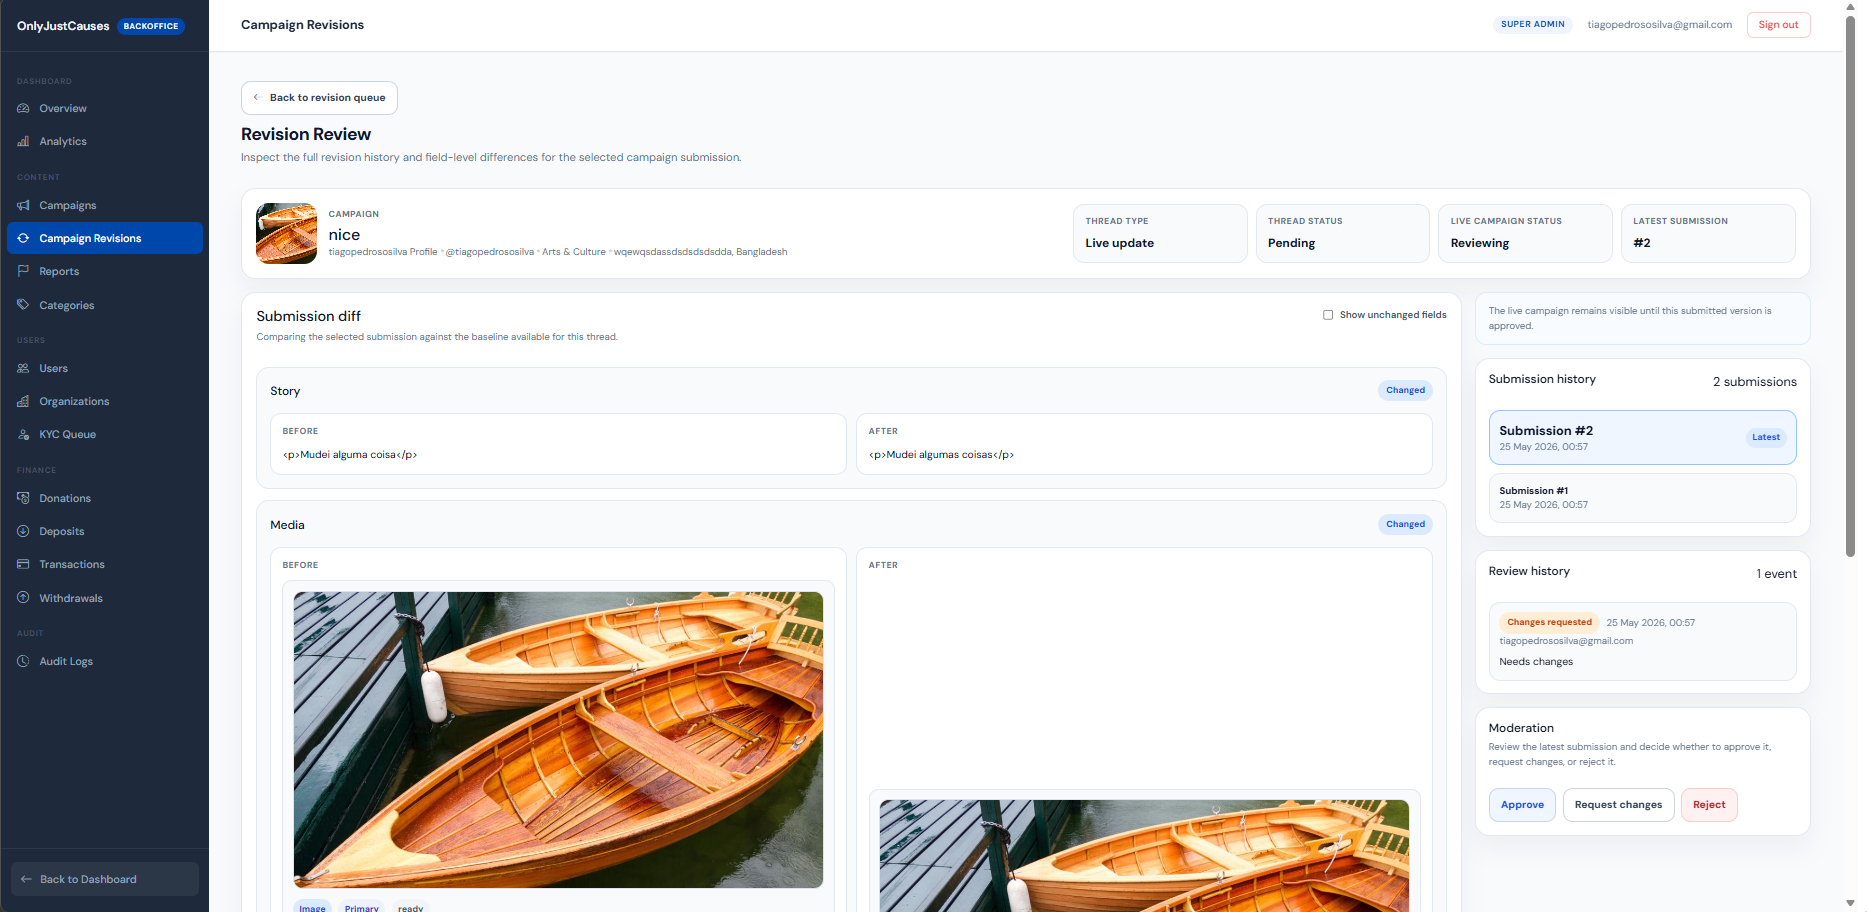
\includegraphics[width=0.95\textwidth, keepaspectratio]{frontmatter/assets/backoffice/ch4/ojc-campaign-review1.png}
\caption{Vista geral de uma \textit{thread} de revisão de campanha}
\label{fig:impl_ojc_campaign_review_thread}
\end{figure}

Depois da Figura~\ref{fig:impl_ojc_campaign_review_thread}, a evidência a reter é que a revisão de campanhas não consiste apenas em alterar um estado numa tabela. A vista reúne o resumo da campanha, o tipo e estado da \textit{thread}, a submissão selecionada, a comparação de conteúdo, o histórico de submissões, o histórico de decisões e as ações de moderação. O operador consegue assim decidir com contexto suficiente e a decisão fica associada à submissão que foi efetivamente analisada.
}{}

\IfFileExists{frontmatter/assets/backoffice/ch4/ojc-campaign-review2.png}{
\begin{figure}[H]
\centering
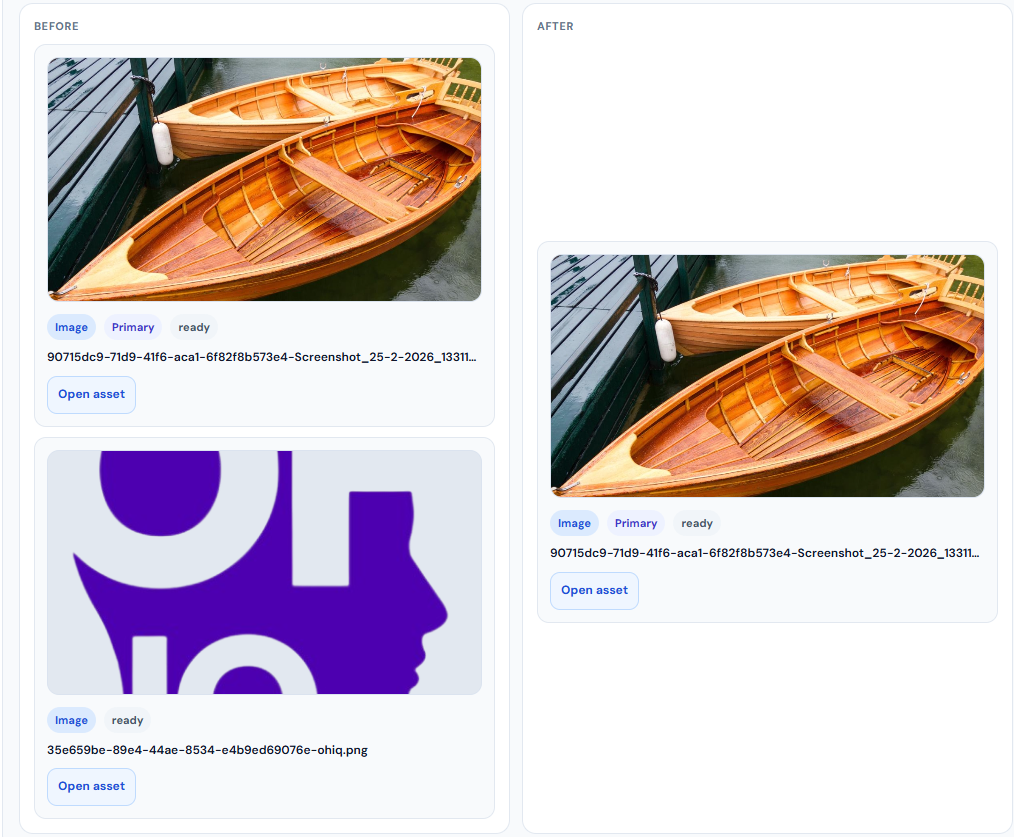
\includegraphics[width=0.82\textwidth, keepaspectratio]{frontmatter/assets/backoffice/ch4/ojc-campaign-review2.png}
\caption{Comparação de elementos multimédia numa revisão de campanha}
\label{fig:impl_ojc_campaign_review_media}
\end{figure}

Depois da Figura~\ref{fig:impl_ojc_campaign_review_media}, a leitura centra-se na comparação entre versões. O painel coloca lado a lado os elementos anteriores e os elementos submetidos, mantendo a indicação de ficheiro principal e o acesso direto ao recurso. Esta apresentação evita que a revisão de imagens dependa apenas da memória do operador ou de uma inspeção manual fora do backoffice.
}{}

\IfFileExists{frontmatter/assets/backoffice/ch4/campaign-review-modal-with-actions.png}{
\IfFileExists{frontmatter/assets/backoffice/ch4/campaign-review-modal-readonly.png}{
\begin{figure}[H]
\centering
\begin{minipage}[t]{0.49\textwidth}
\centering
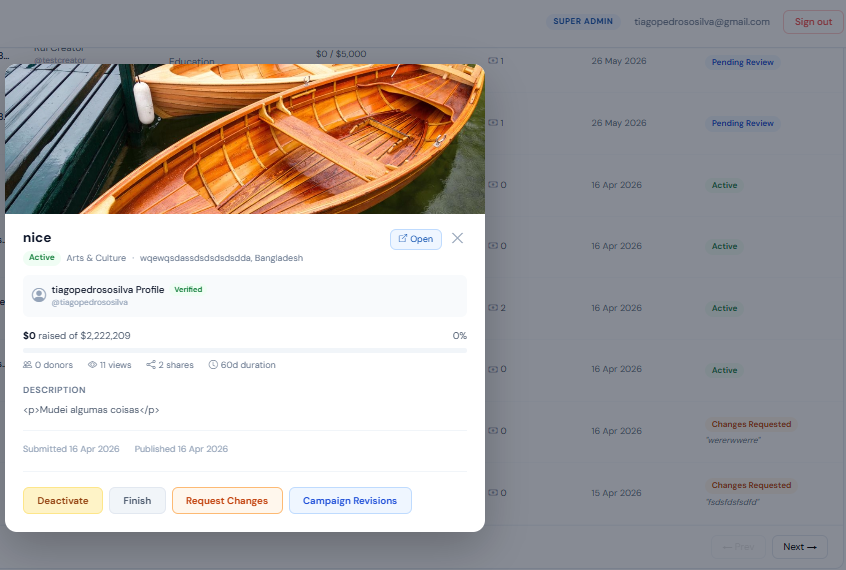
\includegraphics[width=\linewidth, keepaspectratio]{frontmatter/assets/backoffice/ch4/campaign-review-modal-with-actions.png}
{\small Operador com permissões de ação}
\end{minipage}
\hfill
\begin{minipage}[t]{0.49\textwidth}
\centering
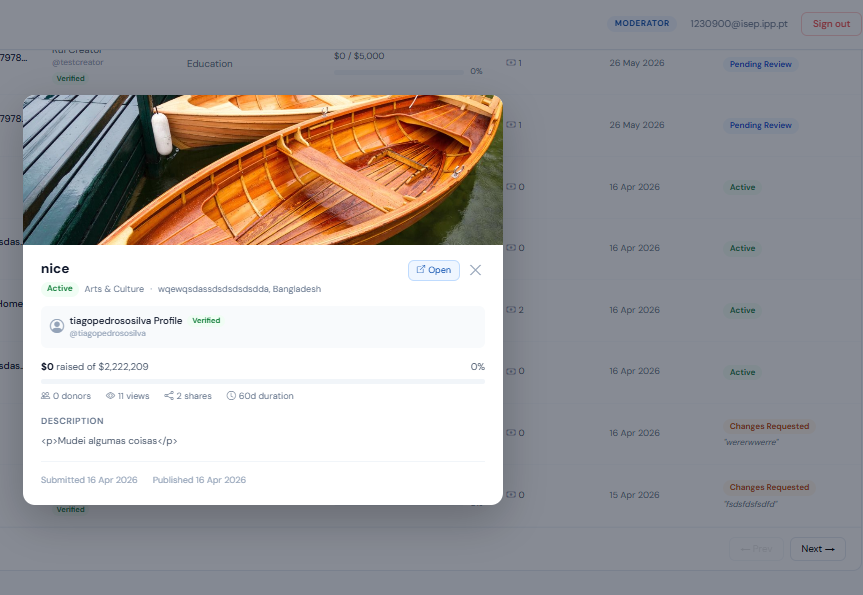
\includegraphics[width=\linewidth, keepaspectratio]{frontmatter/assets/backoffice/ch4/campaign-review-modal-readonly.png}
{\small Operador sem permissões de ação}
\end{minipage}
\caption{Comparação do modal de campanha com e sem permissões de ação}
\label{fig:impl_campaign_modal_permissions}
\end{figure}

Depois da Figura~\ref{fig:impl_campaign_modal_permissions}, a diferença relevante está nas ações disponíveis dentro do mesmo contexto funcional. Ambos os operadores conseguem consultar a campanha, mas apenas o operador com permissões adequadas vê os botões de intervenção, como \texttt{Deactivate}, \texttt{Finish}, \texttt{Request Changes} e \texttt{Campaign Revisions}. Esta evidência completa os exemplos anteriores de autorização: além do acesso à aplicação e à página, o backoffice também controla operações sensíveis dentro de um modal já aberto.
}{}}{}

\IfFileExists{frontmatter/assets/backoffice/ch4/transactional-email.png}{
\begin{figure}[H]
\centering
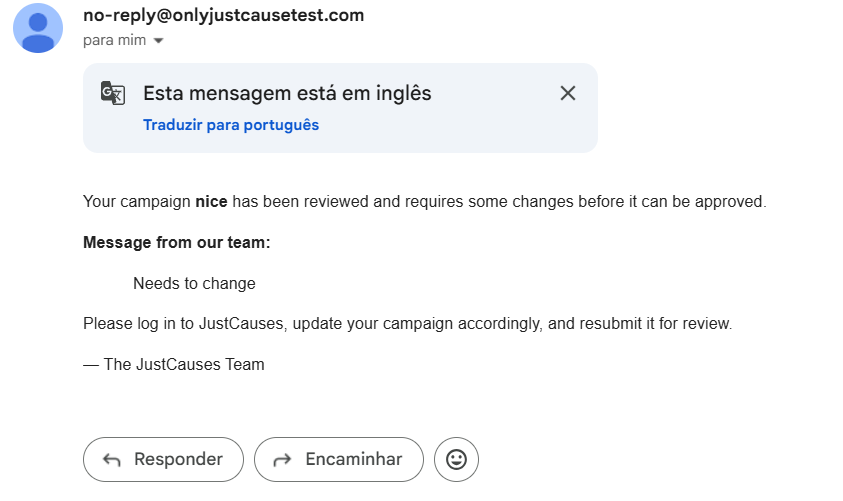
\includegraphics[width=0.82\textwidth, keepaspectratio]{frontmatter/assets/backoffice/ch4/transactional-email.png}
\caption{E-mail transacional enviado após pedido de alterações}
\label{fig:impl_transactional_email}
\end{figure}

Depois da Figura~\ref{fig:impl_transactional_email}, observa-se o resultado externo de uma decisão tomada no painel. A mensagem informa o criador de que a campanha precisa de alterações e inclui a nota definida pelo operador durante a revisão. Este exemplo liga três partes da implementação descritas neste capítulo: decisão administrativa, persistência da mensagem de revisão e envio automático por e-mail.
}{}

\IfFileExists{frontmatter/assets/backoffice/ch4/ojc-categories.png}{
\begin{figure}[H]
\centering
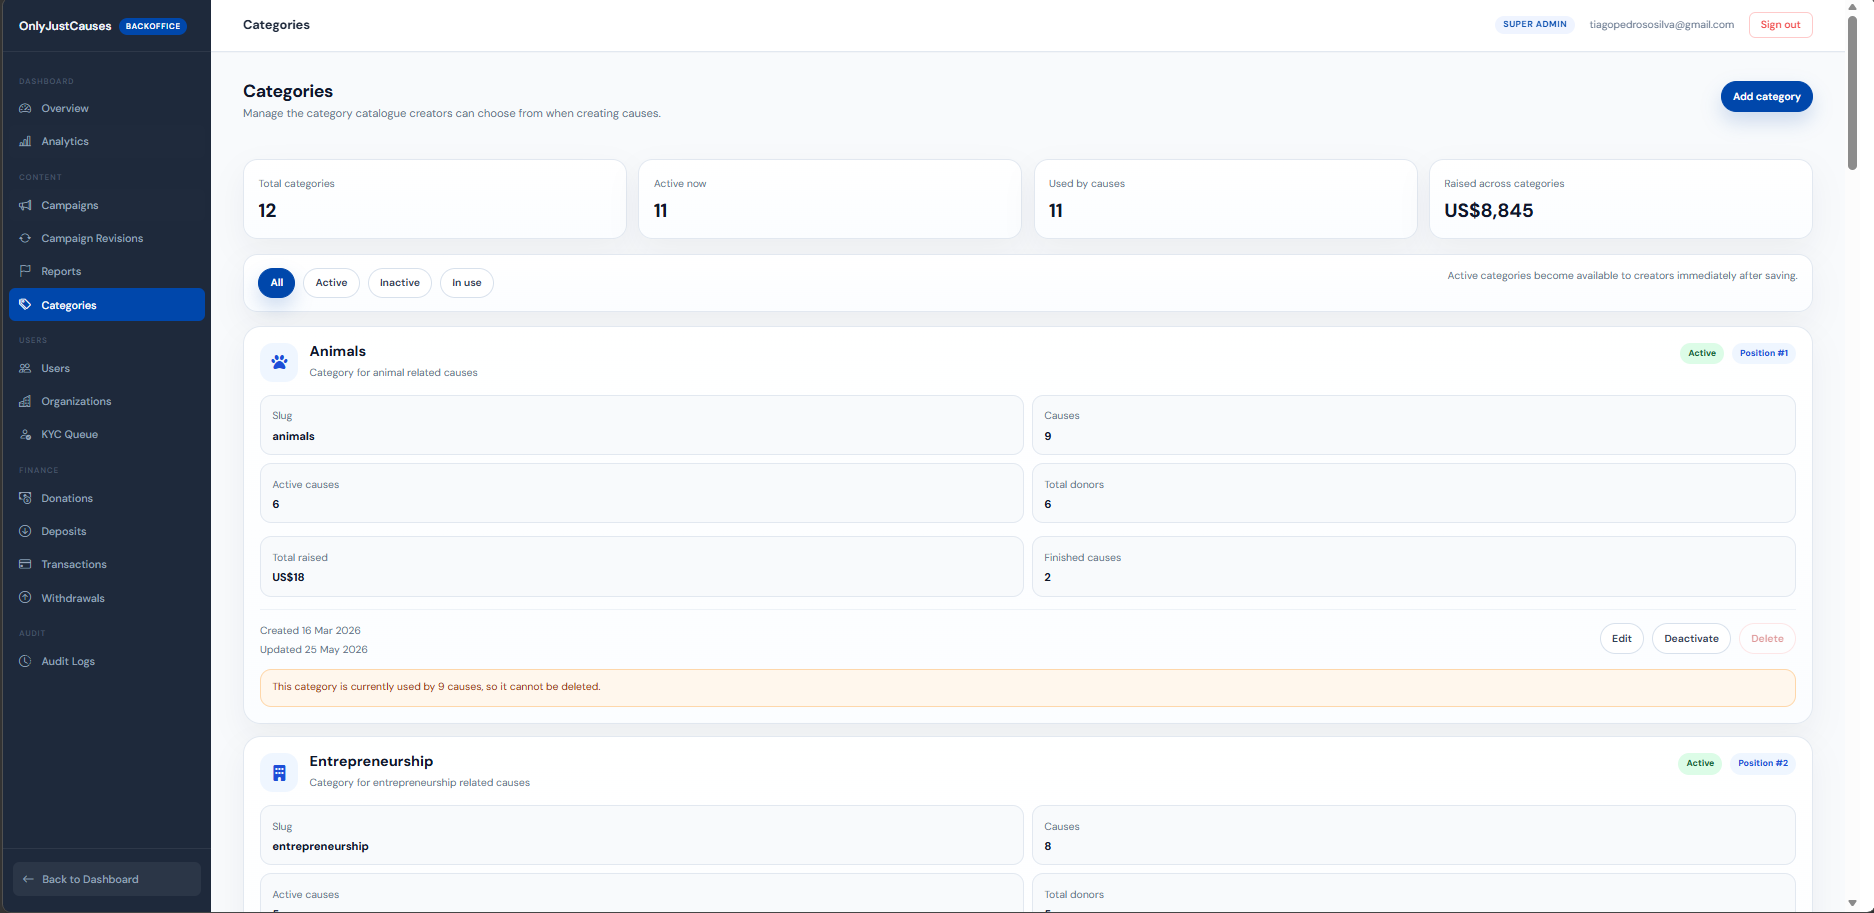
\includegraphics[width=0.95\textwidth, keepaspectratio]{frontmatter/assets/backoffice/ch4/ojc-categories.png}
\caption{Gestão de categorias da JustCauses}
\label{fig:impl_ojc_categories}
\end{figure}

Depois da Figura~\ref{fig:impl_ojc_categories}, a evidência a retirar é que a gestão de categorias não se limita a uma lista de nomes. A página mostra métricas agregadas, filtros por estado, posição de apresentação, número de causas associadas e ações permitidas. Quando uma categoria está em uso, a interface torna explícita a restrição de eliminação, evitando que o operador execute uma ação que afetaria campanhas existentes.
}{}

\IfFileExists{frontmatter/assets/backoffice/ch4/kyc-queue.png}{
\begin{figure}[H]
\centering
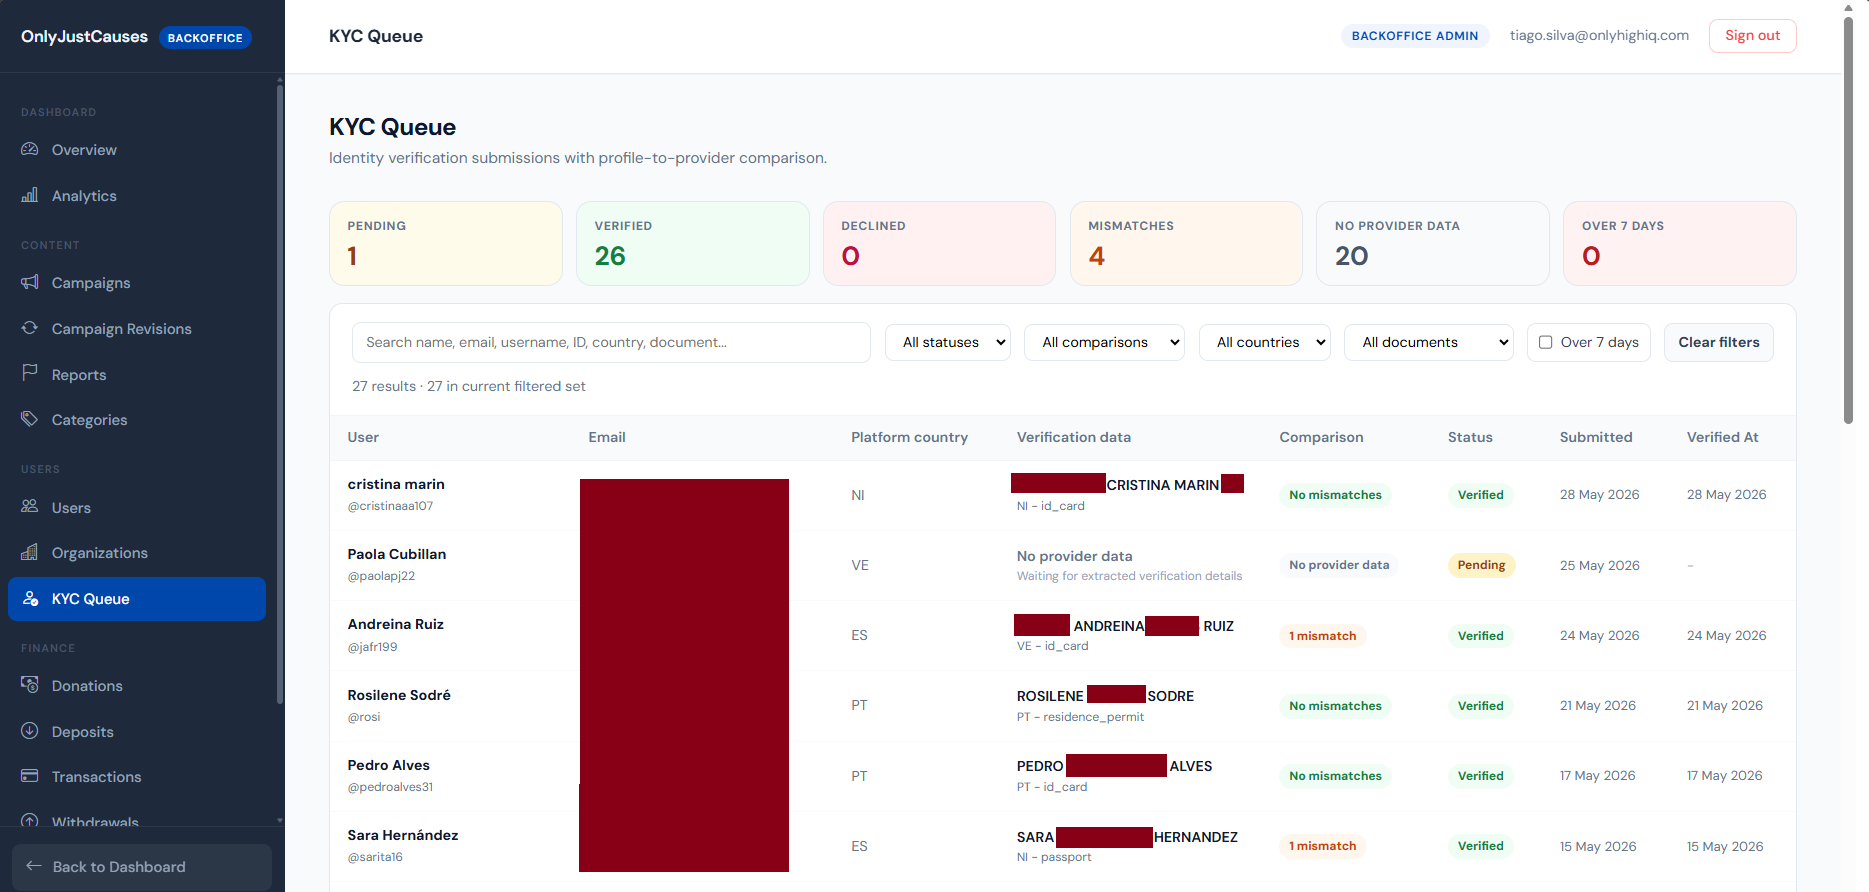
\includegraphics[width=0.95\textwidth, keepaspectratio]{frontmatter/assets/backoffice/ch4/kyc-queue.png}
\caption{Fila de verificação KYC de utilizadores individuais}
\label{fig:impl_kyc_queue}
\end{figure}

Depois da Figura~\ref{fig:impl_kyc_queue}, a evidência principal é a existência de uma fila operacional para acompanhar verificações de identidade. A página permite filtrar submissões por estado, comparação de dados, país, tipo de documento e atraso, mostrando ao operador quais os casos que exigem análise. Esta vista transforma dados provenientes do fornecedor de verificação e dos perfis da JustCauses numa lista acionável dentro do backoffice.
}{}

\IfFileExists{frontmatter/assets/backoffice/ch4/kyc-comparison-modal.png}{
\begin{figure}[H]
\centering
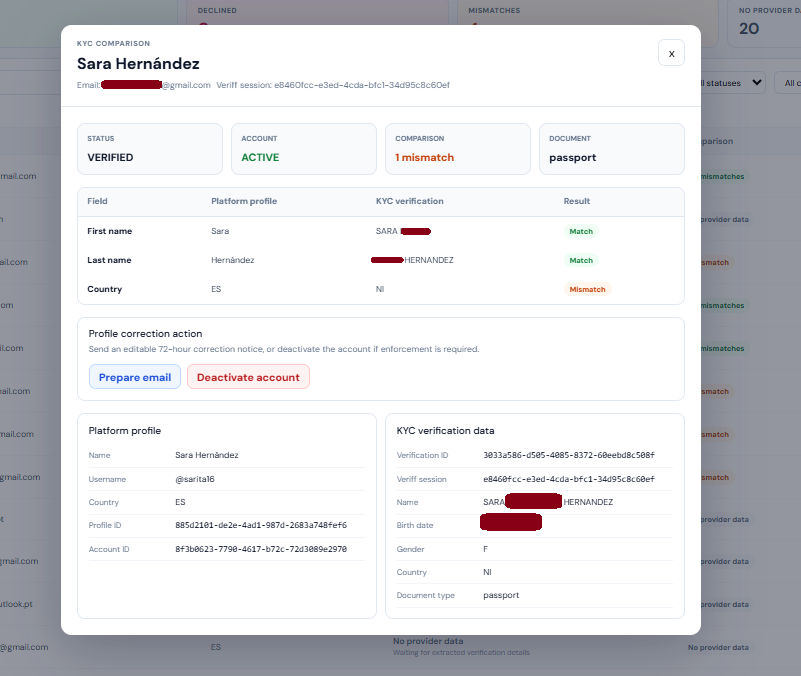
\includegraphics[width=0.78\textwidth, keepaspectratio]{frontmatter/assets/backoffice/ch4/kyc-comparison-modal.png}
\caption{Comparação entre perfil e dados de verificação KYC}
\label{fig:impl_kyc_comparison_modal}
\end{figure}

Depois da Figura~\ref{fig:impl_kyc_comparison_modal}, o ponto a reter é a comparação explícita entre a informação declarada pelo utilizador na plataforma e a informação devolvida pelo fornecedor de verificação. O operador não decide apenas com base no estado final da submissão: vê que campos coincidem, que campos divergem e que ação pode executar. Avisos ao utilizador, reinícios de submissões pendentes e alterações de estado ficam associados a auditoria.
}{}

\IfFileExists{frontmatter/assets/backoffice/ch4/kyb-organizations.png}{
\begin{figure}[H]
\centering
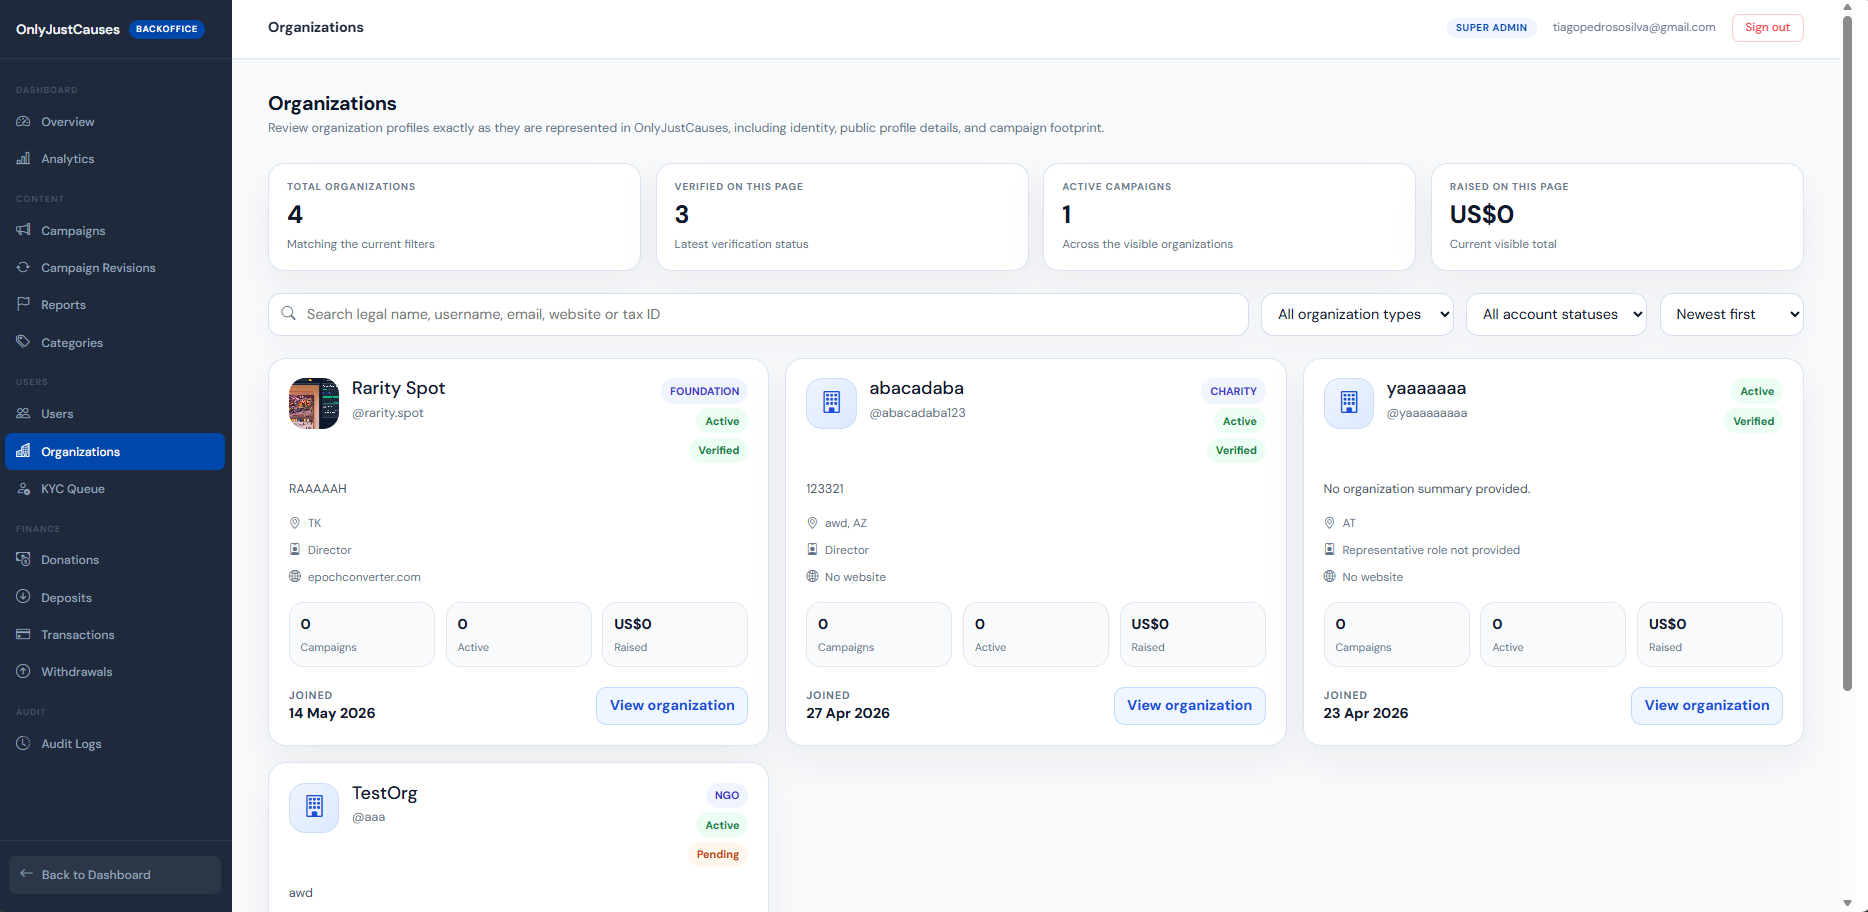
\includegraphics[width=0.95\textwidth, keepaspectratio]{frontmatter/assets/backoffice/ch4/kyb-organizations.png}
\caption{Organizações da JustCauses sujeitas a verificação KYB}
\label{fig:impl_kyb_organizations}
\end{figure}

Depois da Figura~\ref{fig:impl_kyb_organizations}, importa observar que as organizações são apresentadas como perfis coletivos do domínio da JustCauses. A listagem permite localizar entidades, consultar o seu estado operacional e perceber que organizações exigem análise documental. A figura prepara a leitura da verificação \gls{KYB}, sem transformar o módulo numa gestão genérica de organizações.
}{}

\IfFileExists{frontmatter/assets/backoffice/ch4/kyb-verification-modal.png}{
\begin{figure}[H]
\centering
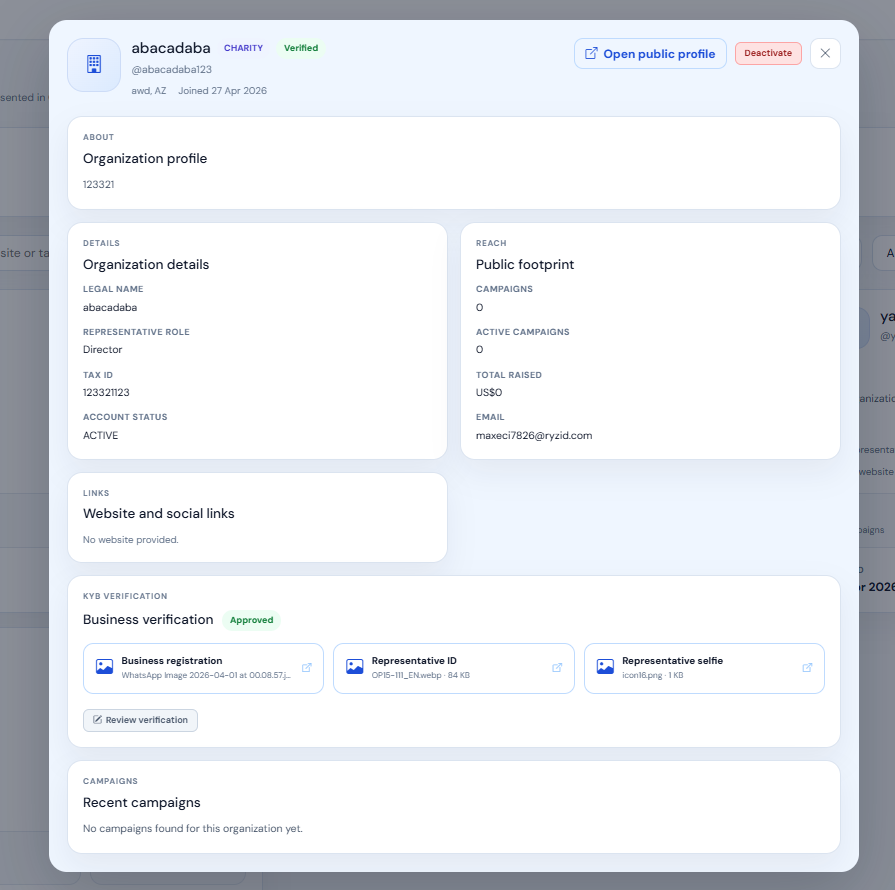
\includegraphics[width=0.72\textwidth, keepaspectratio]{frontmatter/assets/backoffice/ch4/kyb-verification-modal.png}
\caption{Submissão documental KYB de uma organização}
\label{fig:impl_kyb_verification_modal}
\end{figure}

Depois da Figura~\ref{fig:impl_kyb_verification_modal}, a evidência pretendida é a decisão administrativa sobre a oficialidade da organização. O operador consulta dados da entidade, documentos submetidos e estado da verificação antes de aprovar ou rejeitar a submissão. A decisão atualiza o estado de verificação da organização, gera notificação, pode enviar e-mail e fica registada em auditoria.
}{}

%----------------------------------------------------------------------------------------

\section{Testes}
\label{sec:testes}

A validação realizada no âmbito deste estágio combinou duas fontes principais de evidência: validação manual sistemática realizada durante o desenvolvimento e testes automatizados conduzidos pelo elemento da empresa responsável por \gls{QA}. Este relatório descreve a parte executada diretamente no desenvolvimento do backoffice, nomeadamente a utilização dos fluxos na aplicação, a confirmação dos estados apresentados na interface, a verificação das respostas da \gls{API} e a validação dos registos de auditoria gerados.

Os testes automatizados não foram desenvolvidos pelo autor deste relatório. Ainda assim, são relevantes para a avaliação da solução, porque incidem sobre endpoints, fluxos de interface e regras de autorização implementados neste projeto. Esta distinção mantém clara a autoria do trabalho e, ao mesmo tempo, enquadra a validação no processo real da empresa.

\subsection{Validação manual por módulo}
\label{subsec:testes_manual}

A validação manual consistiu em verificar cada módulo após a implementação. Para cada requisito funcional, foram executados cenários de sucesso, cenários de erro, ausência de permissões, persistência de dados e criação dos registos de auditoria esperados. Esta validação incidiu sobre os fluxos transversais de autenticação, autorização, gestão de perfis, \textit{page gates} e auditoria, bem como sobre os módulos da JustCauses. No final do processo, estes cenários foram considerados concluídos no âmbito definido para o estágio. A Tabela~\ref{tab:validacao_manual} resume os principais cenários verificados manualmente.

\begin{table}[H]
\caption{Cenários de validação manual da solução}
\label{tab:validacao_manual}
\begin{center}
\begingroup
\scriptsize
\setlength{\tabcolsep}{4pt}
\begin{tabular}{|>{\raggedright\arraybackslash}p{2.4cm}|>{\raggedright\arraybackslash}p{3.5cm}|>{\raggedright\arraybackslash}p{3.5cm}|>{\raggedright\arraybackslash}p{2.8cm}|}
\hline
\textbf{Módulo} & \textbf{Cenário validado} & \textbf{Resultado esperado} & \textbf{Evidência observada} \\ \hline
Autenticação & Operador inicia sessão com conta ativa & Sessão criada e contexto interno carregado & Redirecionamento para o seletor de aplicações \\ \hline
Acesso a aplicações & Operador sem acesso tenta abrir uma aplicação & Acesso recusado & Ecrã de acesso negado e registo de tentativa \\ \hline
Perfis por aplicação & Administrador atribui perfis a um operador & Só é aceite um perfil por aplicação; backoffice é exclusivo & Atualização persistida e refletida no perfil do utilizador \\ \hline
Permissões & Tentativa de associar permissão de outra aplicação a um perfil & Pedido rejeitado pelo servidor & Resposta de erro e ausência de alteração persistida \\ \hline
\textit{Page gates} & Operador sem permissão tenta aceder a página protegida & Página não é apresentada ou pedido é recusado & Navegação bloqueada e auditoria de recusa \\ \hline
Campanhas & Aprovar, rejeitar ou pedir alterações & Estado atualizado, mensagem registada e auditoria criada & Listagem atualizada e evento de auditoria persistido \\ \hline
Categorias & Criar ou editar categoria & Categoria persistida, duplicados rejeitados & Tabela atualizada ou erro de conflito \\ \hline
KYC/KYB & Rever uma verificação individual ou uma submissão documental de organização & Decisão aplicada, utilizador ou organização notificado e auditoria gerada & Estado de verificação atualizado e evento persistido \\ \hline
Atividade de utilizador & Abrir botão \textbf{Activity} num operador & Histórico filtrável por origem, ação, resultado e aplicação & Modal apresenta logs, audit trail e detalhes \\ \hline
\end{tabular}
\endgroup
\end{center}
\end{table}

Um dos cenários de validação manual incidiu sobre a tentativa de contornar a navegação normal do painel através da introdução direta de uma rota protegida no browser. A Figura~\ref{fig:test_access_denied_manual_route} apresenta esse comportamento para a rota \texttt{/ojc/analytics}, quando acedida por um operador que tem acesso à aplicação JustCauses, mas não tem permissão para essa página específica.

\IfFileExists{frontmatter/assets/backoffice/ch4/access-denied-manual-route.png}{
\begin{figure}[H]
\centering
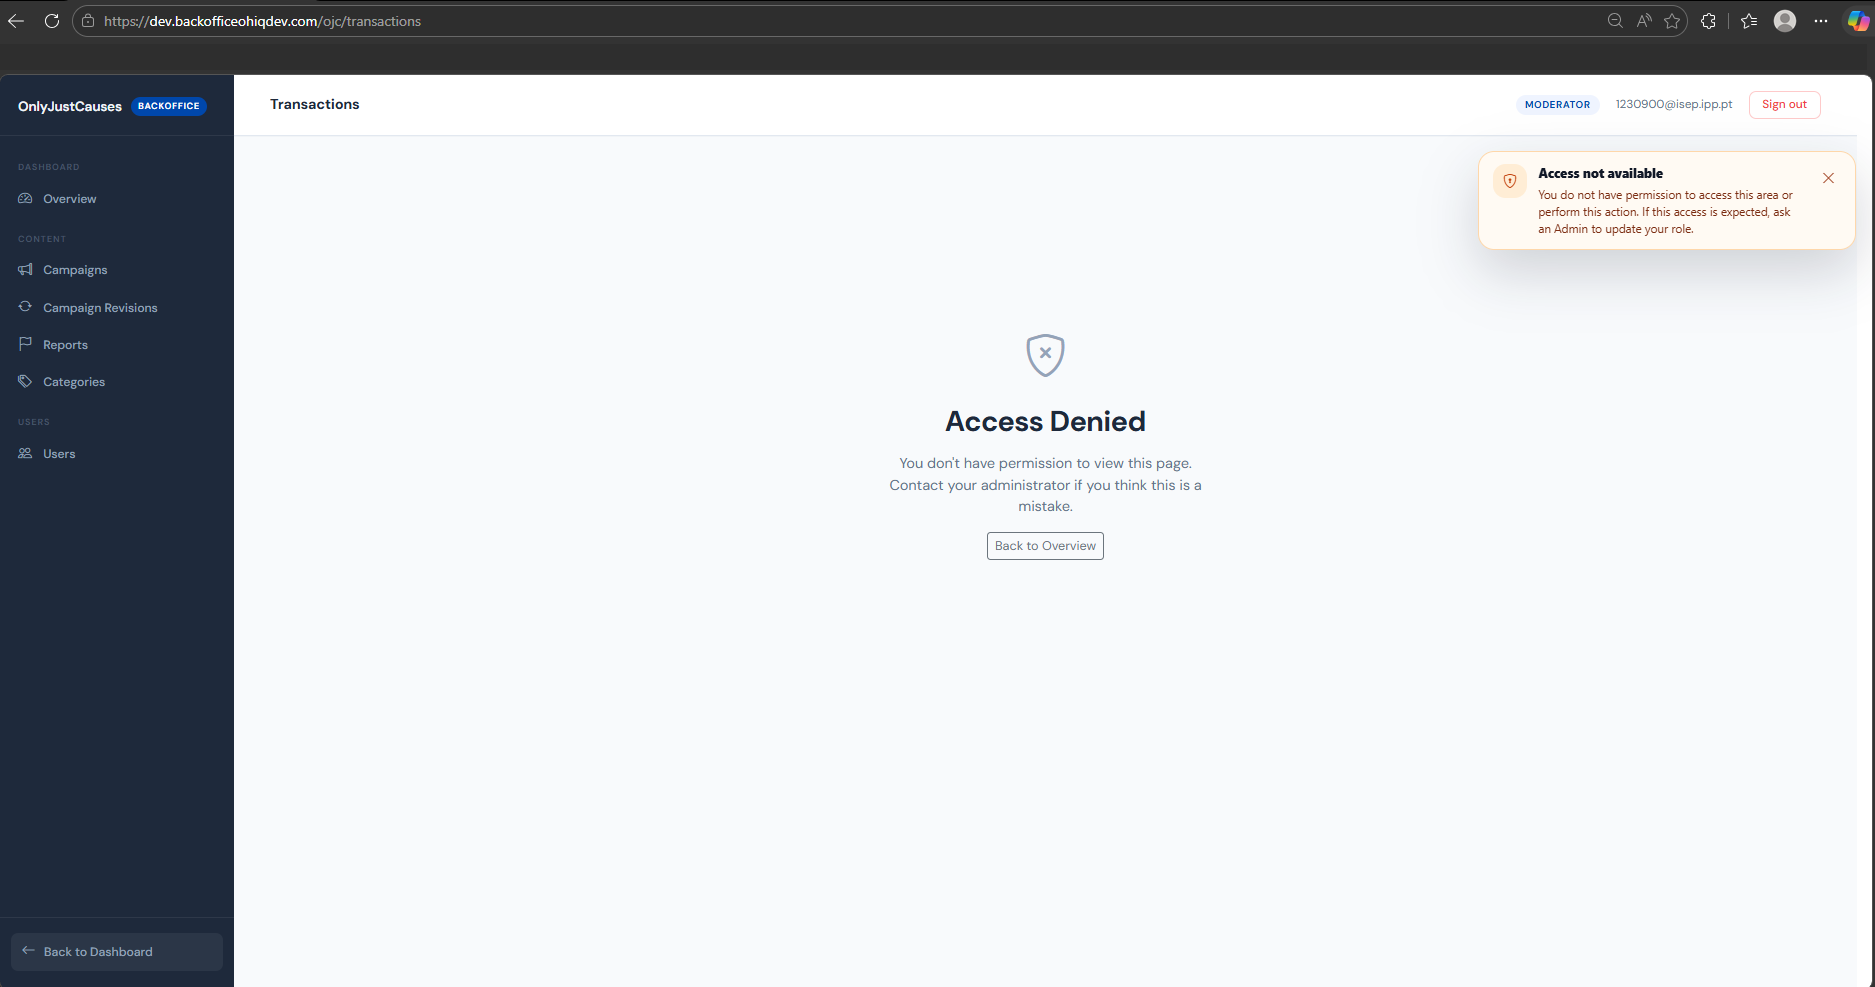
\includegraphics[width=0.95\textwidth, keepaspectratio]{frontmatter/assets/backoffice/ch4/access-denied-manual-route.png}
\caption{Validação manual de acesso negado a página protegida}
\label{fig:test_access_denied_manual_route}
\end{figure}

Depois da Figura~\ref{fig:test_access_denied_manual_route}, a evidência pretendida é que o controlo de acesso não se limita ao nível da aplicação. O operador consegue entrar no painel da JustCauses, mas não consegue abrir uma página para a qual o seu perfil não tem permissão. Mesmo quando a rota é introduzida manualmente, o \textit{page gate} bloqueia a navegação e apresenta um estado de acesso negado. No caso complementar, em que o operador não pertence sequer à aplicação, a validação ocorre antes da renderização do painel interno: é apresentada uma página completa de acesso negado, sem navegação lateral nem separadores da aplicação. Assim, a solução cobre tanto a entrada numa aplicação como o acesso a páginas específicas dentro dessa aplicação. As operações sensíveis continuam a ser verificadas no servidor através do \textit{middleware} de autorização.
}{}

Esta abordagem permitiu acompanhar o ritmo de desenvolvimento das \textit{sprints}, confirmar os fluxos antes da passagem das tarefas para concluído e identificar regressões visíveis durante a fase de testes iniciada a 13 de maio de 2026. A validação manual descrita neste relatório foi complementada pelos testes automatizados realizados pelo colega responsável por essa frente, pelo que a validação da solução ficou concluída dentro do processo de qualidade seguido pela empresa.

\subsection{Testes de código no processo de qualidade}
\label{subsec:testes_qa}

Na empresa, a criação e manutenção dos testes automatizados estava atribuída a um elemento específico da equipa. A sua existência foi importante durante o estágio, porque obrigou a estabilizar contratos de \gls{API}, códigos de resposta, identificadores de interface e estados de erro. Desta forma, as alterações feitas ao modelo de utilizadores, perfis, permissões, \textit{page gates} e auditoria puderam ser avaliadas não apenas por utilização manual, mas também contra cenários automatizados definidos pela equipa de qualidade.

Os artefactos disponíveis estão organizados em três conjuntos. O primeiro conjunto contém testes de \gls{API} em Playwright, focados em autenticação, utilizadores internos, perfis, permissões, \textit{page gates}, logs e estado do serviço. O segundo conjunto contém testes \gls{E2E} em Playwright, executados em browser, que validam fluxos de \textit{login}, \textit{dashboard}, navegação, gestão de utilizadores, auditoria, perfis e configuração de acessos. O terceiro conjunto contém testes de integração em Jest/Supertest, executáveis diretamente contra a \gls{API}, com cenários próximos dos testes de \gls{API}, mas estruturados ao nível de integração de endpoints. A Tabela~\ref{tab:testes_qa} caracteriza estes conjuntos de testes.

\begin{table}[H]
\caption{Caracterização dos testes automatizados de qualidade}
\label{tab:testes_qa}
\begin{center}
\begingroup
\scriptsize
\setlength{\tabcolsep}{4pt}
\begin{tabular}{|>{\raggedright\arraybackslash}p{2.5cm}|>{\raggedright\arraybackslash}p{4.2cm}|>{\raggedright\arraybackslash}p{1.5cm}|>{\raggedright\arraybackslash}p{4.5cm}|}
\hline
\textbf{Conjunto} & \textbf{Âmbito principal} & \textbf{Casos} & \textbf{Resultado ou observação} \\ \hline
\gls{API} Playwright & Autenticação, utilizadores, perfis, permissões, \textit{page gates}, logs e estado do serviço & 223 & Executados no relatório de 27/05/2026, sem falhas, erros ou testes ignorados \\ \hline
\gls{E2E} Playwright & \textit{Login}, \textit{dashboard}, navegação, gestão de operadores, auditoria, perfis e configuração de páginas & 96 & Executados no mesmo relatório, também sem falhas, erros ou testes ignorados \\ \hline
Integração Jest/Supertest & Validação direta de endpoints e contratos da \gls{API} em cenários de integração & 127 & Casos definidos para execução separada, cobrindo os mesmos módulos transversais de administração \\ \hline
\textbf{Total Playwright executado} & \textbf{API + E2E} & \textbf{319} & \textbf{319 testes concluídos com sucesso em 134,6 s, com 0 falhas, 0 erros e 0 ignorados} \\ \hline
\textbf{Total identificado} & \textbf{Playwright + integração} & \textbf{446} & \textbf{Cobertura funcional centrada nos módulos de autenticação, autorização, administração e auditoria} \\ \hline
\end{tabular}
\endgroup
\end{center}
\end{table}

A Listagem~\ref{lst:qa_page_gate_tests} apresenta um excerto representativo dos testes automatizados de \gls{API} sobre a configuração de acesso por página. O exemplo foi escolhido por incidir diretamente sobre uma regra central da solução: os \textit{page gates} pertencem a uma aplicação e a alteração das permissões exigidas deve ficar persistida no servidor. Por concisão, a listagem omite o carregamento inicial do identificador da página e da configuração original, realizado na preparação do teste.

\begin{lstlisting}[caption={Excerto de testes automatizados sobre configuração de acesso por página}, label={lst:qa_page_gate_tests}]
test('deve filtrar por application=just_causes', async ({ request }) => {
  const response =
    await request.get('/api/page-gates?application=just_causes');

  expect(response.status()).toBe(200);
  const gates = await response.json();
  expect(Array.isArray(gates)).toBe(true);

  for (const gate of gates) {
    expect(gate.application).toBe('just_causes');
  }
});

test('a atualizacao deve refletir no GET seguinte', async ({ request }) => {
  if (!gateId) return;
  const newPermissions: string[] = [];

  try {
    await request.put(`/api/page-gates/${gateId}`, {
      data: { requiredPermissions: newPermissions },
    });

    const getResponse =
      await request.get('/api/page-gates?application=just_causes');
    const gates = await getResponse.json();
    const updated = gates.find((g: any) => g.gateId === gateId);

    expect(updated).toBeDefined();
    expect(updated.requiredPermissions).toEqual(newPermissions);
  } finally {
    await request.put(`/api/page-gates/${gateId}`, {
      data: { requiredPermissions: originalPermissions },
    });
  }
});
\end{lstlisting}

O primeiro teste da Listagem~\ref{lst:qa_page_gate_tests} confirma que o filtro por aplicação não devolve configurações de outro domínio. O segundo altera temporariamente as permissões exigidas por uma página, valida a persistência através de uma nova leitura e repõe a configuração original no bloco \texttt{finally}. Este detalhe é relevante num ambiente partilhado, porque permite testar persistência real sem deixar dados artificiais na configuração do backoffice.

O relatório de execução Playwright consultado registou 319 testes concluídos com sucesso, sem falhas, erros, testes ignorados ou testes instáveis. Este resultado cobre os testes de \gls{API} e os testes \gls{E2E}. Os testes de integração em Jest/Supertest constam do conjunto de testes disponível e acrescentam 127 cenários definidos, mas não estavam incluídos no relatório Playwright, por serem executados através de um comando próprio.

Não foi disponibilizado um relatório de cobertura de código por linhas ou instruções. Por esse motivo, a avaliação quantitativa apresentada não deve ser lida como uma percentagem formal de cobertura. O que pode ser concluído com rigor é que existe cobertura funcional automatizada sobre os módulos mais sensíveis do backoffice: autenticação, resolução de utilizador autenticado, criação e manutenção de operadores, perfis, permissões, configuração de páginas, logs, audit trail e navegação administrativa.

Estes testes influenciaram o desenvolvimento de forma concreta. A implementação teve de manter contratos de \gls{API} estáveis, códigos de resposta previsíveis, validações explícitas, estados de erro distinguíveis e identificadores de interface adequados para automação. Isto foi particularmente relevante nas alterações ao modelo de perfis por aplicação e permissões por aplicação, porque os testes obrigam a que a interface, os endpoints e os dados devolvidos continuem alinhados após cada alteração.

%----------------------------------------------------------------------------------------

\section{Avaliação da solução}
\label{sec:avaliacao}

Para além dos testes, a solução foi avaliada pela sua adequação ao problema inicial: permitir operação interna da JustCauses e, simultaneamente, manter uma base técnica reutilizável para futuras aplicações. A disponibilização do backoffice em ambiente de utilização interna permitiu validar a viabilidade operacional dos fluxos principais, sobretudo nos módulos de autenticação, controlo de acesso, auditoria, revisão de campanhas e gestão de categorias.

\subsection{Avaliação operacional e critérios complementares}
\label{subsec:avaliacao_complementar}

A Tabela~\ref{tab:avaliacao_complementar} apresenta os critérios usados para complementar a validação funcional e automatizada.

\begin{table}[H]
\caption{Critérios complementares de avaliação da solução}
\label{tab:avaliacao_complementar}
\begin{center}
\begingroup
\scriptsize
\setlength{\tabcolsep}{4pt}
\begin{tabular}{|>{\raggedright\arraybackslash}p{2.4cm}|>{\raggedright\arraybackslash}p{5.2cm}|>{\raggedright\arraybackslash}p{4.5cm}|}
\hline
\textbf{Critério} & \textbf{Forma de avaliação} & \textbf{Resultado observado} \\ \hline
Adequação funcional & Comparação entre problema inicial, requisitos e funcionalidades implementadas & Os módulos prioritários da JustCauses e os mecanismos transversais de administração ficaram disponíveis no âmbito definido \\ \hline
Segurança e autorização & Validação manual e testes de \gls{API} sobre autenticação, permissões, perfis e acessos negados & A decisão de acesso é aplicada no cliente e revalidada no servidor, com registo auditável das recusas relevantes \\ \hline
Escalabilidade funcional & Verificação do modelo de aplicações, perfis por aplicação, permissões por aplicação e \textit{page gates} & A arquitetura suporta novas aplicações sem duplicar autenticação, autorização e auditoria \\ \hline
Qualidade automatizada & Relatório Playwright e testes de integração disponíveis no processo de \gls{QA} & 319 testes Playwright concluídos com sucesso e 127 testes de integração definidos sobre os módulos transversais \\ \hline
Usabilidade operacional & Utilização interna dos fluxos e revisão dos estados visíveis na interface & As páginas apresentam ações, filtros, estados de erro e mensagens explícitas para apoiar trabalho administrativo diário \\ \hline
Desempenho percebido & Utilização manual dos fluxos principais em ambiente de desenvolvimento e produção interna & Não foram identificados bloqueios funcionais nos fluxos avaliados, embora não tenha sido realizada uma medição formal de carga \\ \hline
Acessibilidade & Revisão visual e funcional dos componentes usados nas páginas principais & Foram mantidos padrões consistentes de navegação e contraste, mas não foi realizada uma auditoria automática formal de acessibilidade \\ \hline
\end{tabular}
\endgroup
\end{center}
\end{table}

Esta avaliação mostra que a solução responde ao núcleo do problema apresentado na introdução: reduzir operações manuais pouco rastreáveis, centralizar a administração da JustCauses e criar uma base de controlo de acesso reutilizável. Ao mesmo tempo, identifica limites da avaliação realizada. Não houve, até ao momento descrito neste relatório, um inquérito formal aos operadores internos nem uma campanha dedicada de testes de carga ou acessibilidade. A avaliação de usabilidade baseou-se, por isso, na utilização operacional e na revisão dos fluxos entregues. Esses instrumentos poderiam complementar a avaliação em iterações futuras, sobretudo quando o número de operadores e aplicações integradas aumentar.

\subsection{Estado final da solução}
\label{subsec:estado_final_solucao}

Esta secção avalia o estado de implementação da solução por eixo funcional, com base no estado do painel no final do período de desenvolvimento coberto por este relatório e nas evidências apresentadas nas secções anteriores. Em vez de voltar a detalhar cada fluxo operacional isolado, a análise centra-se nas capacidades que melhor representam o trabalho efetivamente consolidado e a sua correspondência com os objetivos definidos na introdução. A Tabela~\ref{tab:avaliacao_rf} sintetiza esse estado final.

\begin{table}[H]
\caption{Estado de implementação por eixo funcional}
\label{tab:avaliacao_rf}
\begin{center}
\begingroup
\scriptsize
\setlength{\tabcolsep}{4pt}
\begin{tabular}{|>{\raggedright\arraybackslash}p{2.3cm}|>{\raggedright\arraybackslash}p{3.2cm}|>{\raggedright\arraybackslash}p{1.2cm}|>{\raggedright\arraybackslash}p{1.8cm}|>{\raggedright\arraybackslash}p{3.7cm}|}
\hline
\textbf{Eixo} & \textbf{Descrição resumida} & \textbf{Estado} & \textbf{Obj.} & \textbf{Observações} \\ \hline
Autenticação com Cognito & Gestão de sessão, recuperação de palavra-passe e integração com o painel & Concluído & OE1.1 & Fluxo funcional com Amplify no cliente e validação JWT no servidor \\ \hline
Resolução do contexto de autorização & Perfis, aplicações acessíveis e permissões efetivas do operador & Concluído & OE1.1/OE1.2 & \texttt{/users/me} no cliente e \texttt{req.auth} no servidor mantêm a mesma fonte de verdade \\ \hline
Acesso a aplicações e páginas & Guardas de rota, redireções e \textit{page gates} por aplicação & Concluído & OE1.3/OE2.1 & Separação entre \texttt{backoffice} e \texttt{just\_causes}, com suporte a expansão para novas aplicações \\ \hline
Proteção de endpoints \gls{REST} & Verificação de permissões antes de qualquer operação sensível & Concluído & OE1.3 & \texttt{requirePermission} aplicado de forma consistente nas rotas críticas \\ \hline
Auditoria técnica e funcional & Registo de ações de escrita, acessos negados e atividade por operador & Concluído & OE1.4 & DynamoDB como repositório imutável, audit trail e modal Activity \\ \hline
Dashboard e observabilidade & Visão global da atividade da plataforma & Concluído & OE2.4 & \texttt{AdminOverviewPage} e \texttt{AnalyticsPage} com métricas agregadas \\ \hline
Revisão de campanhas & Aprovação, rejeição e pedido de alterações & Concluído & OE2.2 & Fluxo completo com auditoria e notificação ao criador \\ \hline
Gestão de categorias & Criação, edição e desativação de taxonomias & Concluído & OE2.3 & \gls{CRUD} completo com validação de unicidade \\ \hline
Verificação KYC/KYB & Análise de identidade individual e oficialidade de organizações & Concluído & OE2.5 & Filas e modais de decisão com permissões, notificação, e-mail e auditoria \\ \hline
Configuração administrativa do acesso & Manutenção de contas internas, perfis, permissões e \textit{page gates} & Concluído & OE1.2/OE1.3 & Modelo com um perfil por aplicação, permissões associadas à aplicação e validação no servidor \\ \hline
Validação da solução & Verificação dos fluxos implementados, testes de qualidade e avaliação operacional & Concluído & OP & Validação manual, 319 testes Playwright concluídos com sucesso e utilização interna da solução \\ \hline
\end{tabular}
\endgroup
\end{center}
\end{table}

A análise final desta secção indica que os objetivos estruturais OE1.1 a OE1.5 ficaram concretizados através da autenticação, autorização, controlo de acesso a páginas, proteção de endpoints, auditoria e separação entre dados administrativos e dados operacionais. Os objetivos OE2.1 a OE2.5 ficaram concluídos no âmbito definido para o estágio e demonstram a aplicação da base transversal à JustCauses. Em conjunto, estes resultados suportam o OP.

\section{Sumário}
\label{sec:sumario_cap4}

O trabalho de implementação descrito neste capítulo mostra um painel já utilizável em contexto operacional e, ao mesmo tempo, ainda em evolução. O contributo técnico principal não foi apenas a entrega de páginas, mas a consolidação de uma linha técnica clara para autenticação, autorização, auditoria e administração do acesso.

Esta coerência verifica-se em vários pontos: o \textit{front-end} consome o contexto de acesso calculado pelo \textit{back-end}, as páginas são filtradas por \textit{page gates} configuráveis, os endpoints são revalidados no servidor e as recusas deixam rasto auditável. A evolução para perfis por aplicação reforçou esta base, porque a autorização deixou de depender de um único perfil por utilizador e passou a suportar crescimento controlado para novas aplicações. Os módulos operacionais entregues, incluindo campanhas, categorias, \gls{KYC} e \gls{KYB}, assentam nesta base comum, o que reduz o custo de evolução nas iterações seguintes.

No capítulo seguinte é feita a apreciação global do trabalho realizado, retomando os objetivos inicialmente definidos, as limitações identificadas e as principais linhas de evolução futura da solução.

\chapter{Conclusões}
\label{cap:conclusão}

%----------------------------------------------------------------------------------------

\section{Objetivos concretizados}
\label{sec:objetivos_concretizados}

Este capítulo avalia o grau de concretização dos objetivos definidos no início do estágio, com base nos resultados efetivamente alcançados. A análise retoma o objetivo principal e os objetivos específicos definidos na introdução, usando as capacidades implementadas como evidência da sua concretização. A Tabela~\ref{tab:objetivos} sintetiza essa correspondência.

\begin{table}[H]
\caption{Grau de concretização dos objetivos}
\label{tab:objetivos}
\begin{center}
\scriptsize
\begin{tabular}{|p{1.5cm}|p{4.1cm}|p{1.4cm}|p{5cm}|}
\hline
\textbf{Objetivo} & \textbf{Descrição} & \textbf{Estado} & \textbf{Evidências principais} \\ \hline
OP & Backoffice multiaplicação para o ecossistema OnlyHighIQ & Concluído & Sistema interno operacional, separação entre backoffice de gestão e JustCauses, autenticação centralizada, autorização, auditoria e validação da solução \\ \hline
OE1.1 & Autenticação e contexto administrativo & Concluído & Cognito, gestão de sessão, validação JWT e resolução do operador interno \\ \hline
OE1.2 & Perfis e permissões por aplicação & Concluído & Modelo com um perfil por aplicação, permissões associadas à aplicação e regras próprias para perfis globais de backoffice \\ \hline
OE1.3 & Controlo de acesso coerente & Concluído & Guardas de rota, \textit{page gates}, ações condicionadas na interface e validação por \texttt{requirePermission} \\ \hline
OE1.4 & Auditoria e responsabilização & Concluído & \textit{Audit logs}, \textit{audit trail}, registo de acessos negados e consulta de atividade por operador \\ \hline
OE1.5 & Arquitetura extensível & Concluído & Separação entre dados administrativos do backoffice e dados operacionais da JustCauses, com suporte a novas aplicações \\ \hline
OE2.1 & Integração da JustCauses & Concluído & Aplicação acessível a partir do seletor e separada do backoffice de gestão \\ \hline
OE2.2 & Revisão de campanhas & Concluído & Fluxo de aprovação, rejeição, pedido de alterações, auditoria e notificação ao criador \\ \hline
OE2.3 & Gestão de categorias & Concluído & Criação, edição, desativação e validações operacionais sobre categorias \\ \hline
OE2.4 & Indicadores operacionais & Concluído & Dashboard e \textit{analytics} com métricas agregadas da aplicação \\ \hline
OE2.5 & Verificação KYC/KYB & Concluído & Fila de verificações individuais, análise documental de organizações, notificações, e-mails e auditoria das decisões \\ \hline
\end{tabular}
\end{center}
\end{table}

A análise dos objetivos definidos permite concluir que os elementos estruturantes, autenticação, autorização, controlo de acesso a páginas, auditoria e base arquitetural para crescimento do sistema, ficaram concluídos e coerentes entre si. A evolução para perfis e permissões por aplicação reforçou os objetivos OE1.2 e OE1.5, porque permite administrar a JustCauses sem limitar o backoffice a uma única aplicação. Os módulos operacionais da JustCauses demonstram os objetivos OE2.1 a OE2.5 e funcionam como primeira validação real do OP. A verificação \gls{KYC}/\gls{KYB} reforça esta leitura por combinar dados sensíveis, permissões específicas, decisão administrativa, comunicação externa e auditoria.

%----------------------------------------------------------------------------------------

\section{Limitações e trabalho futuro}
\label{sec:limitacoes_trabalho_futuro}

\subsection{Limitações identificadas}
\label{subsec:limitacoes}

As limitações do trabalho realizado distribuem-se por três dimensões: delimitação do âmbito funcional, natureza da avaliação descrita neste relatório e integração com módulos externos.

\textbf{Âmbito funcional.} O backoffice ficou concluído no âmbito definido para o estágio, mas nem todos os fluxos possíveis do ecossistema da \textit{OnlyHighIQ} foram tratados com o mesmo grau de detalhe. A JustCauses foi a aplicação operacional prioritária e concentrou a maior parte do desenvolvimento funcional. Outros módulos do produto, embora relevantes para a operação futura, ficaram fora do foco principal ou dependiam de decisões de produto e integrações externas que não estavam estabilizadas durante o estágio.

\textbf{Natureza da avaliação.} Durante o estágio, a validação da contribuição própria foi feita manualmente módulo a módulo, através de utilização direta da aplicação, confirmação dos estados apresentados na interface e verificação das respostas das \glspl{API}. A responsabilidade pelos testes automatizados estava atribuída a outro elemento da empresa, mas os artefactos de \gls{QA} disponíveis permitiram caracterizar o conjunto de testes sobre o backoffice, incluindo 319 testes Playwright concluídos com sucesso e 127 testes de integração definidos. Não foi disponibilizada uma medição final de cobertura de código por linhas ou instruções. Também não foi realizado um inquérito formal aos operadores internos nem uma campanha dedicada de testes de carga ou acessibilidade. Assim, a avaliação apresentada combina validação funcional, evidência automatizada de qualidade e observação operacional, mas não pretende substituir uma avaliação quantitativa completa de desempenho, usabilidade e cobertura.

\textbf{Integração com serviços externos.} Não foi possível confirmar, no âmbito do estágio, a captura de eventos de \textit{login} bem-sucedido e falhado no fluxo de autenticação do AWS Cognito previsto para auditoria de autenticação. Por esse motivo, a \texttt{AuditTrailPage} filtra apenas eventos gerados após a autenticação. A integração com o AWS Rekognition para moderação automática de imagens foi identificada como desejável, mas não foi incluída no âmbito deste estágio.

\subsection{Trabalho futuro}
\label{subsec:trabalho_futuro}

As direções de trabalho futuro são as seguintes:

\begin{itemize}
  \item \textbf{Extensão do ecossistema}: integrar novas aplicações do ecossistema da \textit{OnlyHighIQ} no mesmo painel de administração, aproveitando a separação já existente entre módulos transversais e módulos específicos de cada aplicação.

  \item \textbf{Avaliação de micro-frontends}: estudar, numa fase futura, a possibilidade de separar cada aplicação integrada num micro-frontend próprio. Esta alternativa aumentaria o isolamento e a independência de evolução por aplicação, mas também traria mais custos de infraestrutura, \textit{deploy}, manutenção e coordenação técnica. Por esse motivo, não foi adotada nesta fase.

  \item \textbf{Notificações em tempo real}: implementar um canal de notificações para operadores baseado em \gls{SSE} ou WebSocket, que informe em tempo real sobre eventos operacionais relevantes.

  \item \textbf{Exportação e apoio à auditoria}: acrescentar exportação para \gls{PDF} e \gls{CSV} nos módulos operacionais e de observabilidade, reforçando o suporte a auditorias internas e externas.

  \item \textbf{Avaliação operacional contínua}: recolher métricas de utilização, feedback estruturado de operadores internos, medições automáticas de desempenho e auditorias formais de acessibilidade.

  \item \textbf{Integrações inteligentes}: avaliar a integração do AWS Rekognition e de serviços semelhantes para triagem automática de conteúdo e deteção precoce de padrões anómalos.
\end{itemize}

%----------------------------------------------------------------------------------------

\section{Apreciação final}
\label{sec:apreciacao_final}

O estágio na \textit{OnlyHighIQ} permitiu aplicar conhecimentos técnicos e metodológicos num contexto profissional de produto. Ao longo de aproximadamente 14 semanas, foi possível conceber, arquitetar e implementar um sistema de administração multiaplicação, validado através da integração operacional com uma plataforma de \textit{crowdfunding} real e preparado para crescer com o restante ecossistema da empresa.

Do ponto de vista técnico, o principal desafio foi a integração entre múltiplas bases de dados (PostgreSQL partilhado da JustCauses e DynamoDB para configuração e auditoria) e a gestão de permissões multiaplicação com um único sistema de autenticação Cognito. A implementação da resolução central de acesso, baseada em \texttt{roleIds}, permissões por aplicação e validação no \textit{middleware} \texttt{requirePermission}, exigiu um entendimento aprofundado do ciclo de pedido HTTP do Express 5 e das garantias de consistência eventual do DynamoDB. A gestão de múltiplos \textit{connection pools} PostgreSQL (partilhado e OJC) com TypeDI exigiu também estudo e iteração.

O desenvolvimento do modelo de permissões ultrapassou uma abordagem centrada apenas em operações \gls{CRUD}. A solução exigiu alinhar Cognito, dados internos de utilizadores, navegação React, \textit{page gates} configuráveis, perfis globais de backoffice, permissões por aplicação e registo de tentativas falhadas com controlo de redundância na auditoria. Esta componente aproximou o projeto de um sistema de produção, com regras transversais aplicadas de forma consistente entre cliente, servidor e persistência.

A nível profissional, o trabalho em metodologia SCRUM com \textit{sprints} semanais e gestão de tarefas no Jira reforçou competências de entrega iterativa. A necessidade de comunicar bloqueadores ao supervisor, estimar esforço de implementação e documentar decisões de design em comentários de \textit{issue} contribuiu para o desenvolvimento progressivo de práticas de trabalho em equipa.

A experiência na \textit{OnlyHighIQ} permitiu trabalhar num contexto de autonomia técnica e responsabilidade individual. O facto de trabalhar sobre uma base de código existente, com decisões de arquitetura já tomadas e padrões a respeitar, exigiu compreender o sistema antes de o estender. O resultado final é um backoffice operacional, utilizável pela JustCauses e preparado para crescer com o ecossistema da empresa, com autenticação centralizada, controlo de acesso consistente, auditoria e módulos operacionais prioritários já disponíveis, incluindo revisão de campanhas, categorias, indicadores operacionais e verificação \gls{KYC}/\gls{KYB}.


%----------------------------------------------------------------------------------------
%	BIBLIOGRAPHY
%----------------------------------------------------------------------------------------

\printbibliography[heading=bibintoc]

%----------------------------------------------------------------------------------------
%	THESIS CONTENT - APPENDICES
%----------------------------------------------------------------------------------------

\appendix % Cue to tell LaTeX that the following "chapters" are Appendices

% Include the appendices of the thesis as separate files from the Appendices folder
% Uncomment the lines as you write the Appendices

\chapter{Diagramas de sequência}
\label{app:sd_detalhados}

Este apêndice reúne diagramas de sequência detalhados (\gls{SD}) associados aos componentes de Nível 3 apresentados no Capítulo~\ref{cap:analise_desenho}. No corpo do capítulo são apresentados apenas dois \glspl{SSD} de Nível 1, escolhidos por representarem o núcleo transversal de acesso/autorização e um fluxo operacional da JustCauses. Os diagramas deste apêndice expandem esses e outros fluxos concretos ao nível técnico, mostrando a interação entre interface, rotas, controladores, serviços, repositórios, persistência, auditoria e serviços externos. A sua colocação em apêndice permite documentar a implementação sem interromper a leitura principal da arquitetura. As Figuras~\ref{fig:sd_login_full} a~\ref{fig:sd_kyb_verification_full} apresentam esses fluxos detalhados.

%----------------------------------------------------------------------------------------

\section{Resolução de acesso após autenticação}
\label{app:sd_login_full}

A Figura~\ref{fig:sd_login_full} detalha a passagem entre a autenticação do operador e a resolução inicial do seu contexto de autorização no backoffice.

\begin{figure}[H]
\centering

\includegraphics[width=\textwidth, height=0.85\textheight, keepaspectratio]{frontmatter/assets/backoffice/ch3/uml/login-authentication/ssd-full}
\caption{SD detalhado: resolução de acesso após autenticação}
\label{fig:sd_login_full}
\end{figure}

%----------------------------------------------------------------------------------------

\section{Criação de operadores administrativos}
\label{app:sd_create_admin_full}

A Figura~\ref{fig:sd_create_admin_full} detalha a criação de um operador administrativo e o registo da ação.

\begin{figure}[H]
\centering

\includegraphics[width=\textwidth, height=0.85\textheight, keepaspectratio]{frontmatter/assets/backoffice/ch3/uml/create-admin-user/ssd-full}
\caption{SD detalhado: criação de operador administrativo}
\label{fig:sd_create_admin_full}
\end{figure}

%----------------------------------------------------------------------------------------

\section{Atribuição de perfis por aplicação}
\label{app:sd_role_assignment_full}

A Figura~\ref{fig:sd_role_assignment_full} detalha a validação e a persistência da atribuição de perfis por aplicação.

\begin{figure}[H]
\centering

\includegraphics[width=\textwidth, height=0.85\textheight, keepaspectratio]{frontmatter/assets/backoffice/ch3/uml/CH4-ROLE-ASSIGNMENT/ssd-full}
\caption{SD detalhado: atribuição de perfis a um operador}
\label{fig:sd_role_assignment_full}
\end{figure}

%----------------------------------------------------------------------------------------

\section{Gestão de perfis e permissões}
\label{app:sd_roles_permissions_full}

A Figura~\ref{fig:sd_roles_permissions_full} detalha o carregamento, edição e gravação de perfis e permissões.

\begin{figure}[H]
\centering

\includegraphics[width=\textwidth, height=0.85\textheight, keepaspectratio]{frontmatter/assets/backoffice/ch3/uml/roles-permissions/ssd-full}
\caption{SD detalhado: carregamento e edição de perfis e permissões}
\label{fig:sd_roles_permissions_full}
\end{figure}

%----------------------------------------------------------------------------------------

\section{Configuração de page gates}
\label{app:sd_page_gates_full}

A Figura~\ref{fig:sd_page_gates_full} detalha a configuração administrativa das permissões necessárias para aceder a páginas.

\begin{figure}[H]
\centering

\includegraphics[width=\textwidth, height=0.85\textheight, keepaspectratio]{frontmatter/assets/backoffice/ch3/uml/CH4-PAGE-GATES/ssd-full}
\caption{SD detalhado: configuração administrativa de page gates}
\label{fig:sd_page_gates_full}
\end{figure}

%----------------------------------------------------------------------------------------

\section{Atividade individual de operadores}
\label{app:sd_user_activity_full}

A Figura~\ref{fig:sd_user_activity_full} detalha a agregação dos registos de atividade associados a um operador.

\begin{figure}[H]
\centering

\includegraphics[width=\textwidth, height=0.85\textheight, keepaspectratio]{frontmatter/assets/backoffice/ch3/uml/CH4-USER-ACTIVITY/ssd-full}
\caption{SD detalhado: agregação de atividade de um operador}
\label{fig:sd_user_activity_full}
\end{figure}

%----------------------------------------------------------------------------------------

\section{Revisão de campanhas e comunicação}
\label{app:sd_campaign_revision_full}

A Figura~\ref{fig:sd_campaign_revision_full} detalha a decisão de revisão de campanha, a notificação e o envio de e-mail.

\begin{figure}[H]
\centering

\includegraphics[width=\textwidth, height=0.85\textheight, keepaspectratio]{frontmatter/assets/backoffice/ch3/uml/CH4-CAMPAIGN-REVISION/ssd-full}
\caption{SD detalhado: thread de revisão de campanha com notificação e e-mail}
\label{fig:sd_campaign_revision_full}
\end{figure}

%----------------------------------------------------------------------------------------

\section{Gestão de categorias}
\label{app:sd_categories_full}

A Figura~\ref{fig:sd_categories_full} detalha as operações de gestão de categorias e respetiva auditoria.

\begin{figure}[H]
\centering

\includegraphics[width=\textwidth, height=0.85\textheight, keepaspectratio]{frontmatter/assets/backoffice/ch3/uml/manage-categories/ssd-full}
\caption{SD detalhado: gestão de categorias}
\label{fig:sd_categories_full}
\end{figure}

%----------------------------------------------------------------------------------------

\section{Verificação KYC de utilizadores individuais}
\label{app:sd_kyc_verification_full}

A Figura~\ref{fig:sd_kyc_verification_full} detalha o fluxo de verificação KYC de utilizadores individuais.

\IfFileExists{frontmatter/assets/backoffice/ch3/uml/kyc-verification/ssd-full.png}{
\begin{figure}[H]
\centering

\includegraphics[width=\textwidth, height=0.85\textheight, keepaspectratio]{frontmatter/assets/backoffice/ch3/uml/kyc-verification/ssd-full}
\caption{SD detalhado: verificação KYC de utilizadores individuais}
\label{fig:sd_kyc_verification_full}
\end{figure}
}{}

%----------------------------------------------------------------------------------------

\section{Verificação KYB de organizações}
\label{app:sd_kyb_verification_full}

A Figura~\ref{fig:sd_kyb_verification_full} detalha o fluxo de verificação KYB de organizações.

\IfFileExists{frontmatter/assets/backoffice/ch3/uml/kyb-verification/ssd-full.png}{
\begin{figure}[H]
\centering

\includegraphics[width=\textwidth, height=0.85\textheight, keepaspectratio]{frontmatter/assets/backoffice/ch3/uml/kyb-verification/ssd-full}
\caption{SD detalhado: verificação KYB de organizações}
\label{fig:sd_kyb_verification_full}
\end{figure}
}{}

%\input{appendices/appendixB}
%\input{appendices/appendixC}

%----------------------------------------------------------------------------------------
%	THE DOCUMENT ENDS HERE
%----------------------------------------------------------------------------------------

\end{document}
